\documentclass[preprint]{article}
\usepackage{neurips_2025}
\usepackage{amsmath,amssymb}
\usepackage{graphicx}
\usepackage{booktabs}
\usepackage{multirow}
\usepackage{xcolor}
\usepackage{enumitem}
% hyperref loaded by neurips_2025.sty with colorlinks options
\usepackage{tcolorbox}
\usepackage{microtype}
\usepackage{xurl}           % allow URL line breaks at any character
\usepackage{placeins}
\usepackage{float}

% For compact lists
\setlist{nosep}

% Prevent widow/orphan lines
\widowpenalty=10000
\clubpenalty=10000


\title{Safety Under Scaffolding: How Evaluation Conditions Shape Measured Safety}

\author{
  Dr.\ David Gringras \\
  Harvard University \\
  \texttt{davidgringras@hsph.harvard.edu} \\
  \texttt{davidgri@mit.edu} \\
}

\begin{document}

\maketitle
\thispagestyle{firstpage}

% ===========================================================================
% ABSTRACT
% ===========================================================================
\begin{abstract}
A safety score earned on a benchmark need not predict how the same model behaves once it is wrapped in an agentic scaffold the benchmark never tested.

The primary scaffold experiment ran six frontier models through four deployment configurations (direct API, ReAct, multi-agent critic, and map-reduce delegation), generating $N = 62{,}808$ scored evaluations across four pre-registered safety benchmarks (BBQ, TruthfulQA, XSTest/OR-Bench, and sycophancy).  Three additional analyses on the same models and methodology extend the design: an AI factual-recall control ($N = 12{,}000$), a Phase~2 mechanistic probe ($N = 7{,}200$), and a format-dependence experiment ($N = 4{,}400$).  All analyses were blinded, used equivalence testing, and were pre-specified by a specification-curve apparatus; the dataset map opening Section~\ref{sec:overview} gives sample contributions for every estimate.

The scaffold study finds a split across architectures.  Two of the three (ReAct and multi-agent) sit inside the pre-registered $\pm 2$~pp equivalence margin in pooled estimates --- ReAct's effect is statistically significant on Holm correction but still TOST-equivalent, and multi-agent is non-significant and TOST-equivalent; map-reduce delegation degrades pooled measured safety with NNH~$=14$ (about one additional benchmark failure per fourteen cases routed through naive map-reduce, on the four-benchmark mix tested).

On the same items, posing a benchmark question in multiple-choice form versus open-ended form shifts the measured safety rate by 5--20 percentage points, and not always in the same direction.  MC understates measured safety on BBQ ($+16.2$~pp gap to OE) and sycophancy ($+19.6$~pp); MC overstates capability on MMLU by 9.2~pp; the AI factual-recall control sits at $-1.0$~pp, the within-study negative control on judge-leniency the design demands.  With format kept constant, the scaffold contributions are essentially flat at the pooled level.

That leaves a three-source decomposition of the map-reduce loss.  Approximately 40--89\% of the per-model loss is format-contingent measurement (decomposition strips MC options from worker sub-calls and the worker then answers in effective open-ended form, which the benchmark scores against an MC key).  The remaining 11--60\% is genuine reasoning disruption under task delegation and varies by model: Opus carries the smallest residual (11\%, an order-of-magnitude decrease once format is restored), while GPT-5.2 carries the largest (60\%).  Scoring methodology sensitivity is the third channel: negligible under our pre-registered LLM-as-judge protocol, but heuristic refusal classification would have manufactured or reversed five distinct findings.  One relatively inexpensive engineering modification (propagating MC options throughout all sub-calls) recovers most of the lost value (40--89\% across the four models with substantial gaps) on the two benchmarks where it was tested.

Past the format channel, the remainder of the loss components follows a depth-of-encoding gradient.  Properties with high baseline safety rates survive scaffolding; sycophancy, the property with by far the lowest baseline (29.2\% non-sycophantic at direct API), is also the only one where all three scaffolds improve safety on aggregate ($+2.1$ to $+2.5$~pp), and where model-by-scaffold heterogeneity reaches 35.6~pp (Opus loses 16.8~pp under map-reduce; on the same items, Llama~4 gains 18.8~pp).

Outside literature lines up with the result.  Sycophancy is linked to reward tampering~\cite{denison2024sycophancy}; reward tampering, in turn, generalises to emergent misalignment under agentic deployment~\cite{taylor2025school, macdiarmid2025emergent}.  The property implicated in the worst-case escalation pathway is, on our data, the property whose scaffold response we cannot predict in sign or magnitude without per-model, per-configuration testing.

A factorial variance decomposition arrives at the same picture: scaffold architecture accounts for only $0.4\%$ of total outcome variance, the least systematic factor in the design (benchmark selection explains roughly $45\times$ more, at $19.3\%$); the scaffold$\times$benchmark interaction is approximately $3\times$ larger than the scaffold main effect ($1.2\%$); the generalizability analysis returns $G = 0.000$ with bootstrap-based 95\% CI $[0.000, 0.752]$.  The interval is wide by design.  With only four benchmarks, composite reliability cannot be distinguished from zero, but neither can it be ruled out as moderate under a richer mix.  Either way, an interval spanning ``of little use'' to ``very good'' is by itself sufficient to defeat a single composite safety metric as a basis for deployment decisions.

A note on scope.  Bias, sycophancy, truthfulness, and over-refusal are the easy cases: established benchmarks, deterministic scoring on three of four, eighteen pre-specified falsification tests against the format-dependence finding, zero outright failures.  Consequential safety properties (scheming, deceptive alignment, CBRN uplift) have none of these advantages and no obvious reason to be less format- or scaffold-sensitive than the proxies.

Code, data, and prompts are released as \textsc{ScaffoldSafety}.
\end{abstract}

\begin{tcolorbox}[colback=blue!3, colframe=blue!50!black, title=\textbf{Key Findings}, fonttitle=\small\sffamily, boxrule=0.5pt, arc=2pt]
\small
\begin{itemize}[leftmargin=*, nosep, itemsep=2pt]
    \item \textbf{Map-reduce delegation degrades pooled safety} (NNH~$=14$ on the four-benchmark mix), mainly because the decomposition function removes MC options and the worker sub-agent uses an effective open-ended style that the benchmarks then score against an MC key.  An option-preserving version of map-reduce was able to recover approximately 40--89\% of the lost safety on the two benchmarks where it was tested; the remaining 11--60\% represents genuine reasoning disruption under delegation and varies across models. [Sections~4--5]
    \item \textbf{Format alone shifts safety scores by 5--20\,pp on identical items.}  MC \emph{understates} measured safety on BBQ (gap to OE $+16.2$\,pp) and sycophancy ($+19.6$\,pp); MC \emph{overstates} capability on MMLU by 9.2\,pp; AI factual recall is format-invariant ($-1.0$\,pp), which is what a within-study judge-leniency control should look like.  Within-format scaffold contrasts are pooled-flat. [Section~5]
    \item \textbf{Sycophancy exhibits the lowest baseline level of any property assessed} (29.2\% non-sycophantic at the direct API; 6--49\% among models).  It is also the only property where all three scaffolds increase safety in aggregate.  The model-by-scaffold interaction is the largest in the study: Opus decreased by 16.8\,pp and Llama~4 gained 18.8\,pp under map-reduce on the same items. [Section~6]
    \item \textbf{There was considerable variation in how individual models respond to different scaffolding techniques} (spanning 35.6\,pp); the magnitude is enough to defeat any universal claim about whether scaffolding improves or degrades safety.  Coupled with sycophancy's causal connection to reward tampering and emergent misalignment~\cite{denison2024sycophancy, taylor2025school, macdiarmid2025emergent}, this is the empirical case for per-configuration testing as a floor, not a ceiling. [Section~4]
    \item \textbf{Scaffold architecture explains $0.4\%$ of outcome variance} ($45\times$ less than benchmark choice); the generalizability analysis returns $G = 0.000$ with bootstrap 95\% CI $[0.000, 0.752]$.  That range alone defeats any single composite safety number as a deployment input, without establishing that the true reliability is zero. [Appendix~\ref{app:gtheory}]
\end{itemize}
\end{tcolorbox}


% ===========================================================================
% TABLE OF CONTENTS
% ===========================================================================
{
\hypersetup{linkcolor=black}
\setcounter{tocdepth}{2}
\tableofcontents
}

\clearpage

% ===========================================================================
% 1. INTRODUCTION
% ===========================================================================
\section{Introduction}
\label{sec:intro}

A model that scores 83\% on a bias benchmark can score 99\% on the same questions stripped of their answer options.  The model has not changed; the format has.  This paper is about what changes when the evaluation format changes, and about what happens to that format when an agentic scaffold restructures the query before the model ever sees it.  The two questions turn out to be the same question.

\paragraph{Two gaps.}
The first is architectural.  Almost every major benchmark cited in safety evaluations~\cite{lin2022truthfulqa, parrish2022bbq, rottger2024xstest} and almost every responsible-scaling framework~\cite{anthropicrsp2026} and almost every third-party assessment examines a model as a standalone function: prompt in, response out, score.  Real-world production models are not standalone functions.  They sit inside agentic scaffolds that add reasoning traces~\cite{yao2023react}, run them through critic agents~\cite{du2024improving}, or decompose tasks across delegation pipelines.  Each restructures the input, and therefore changes, in principle, what the safety benchmark is measuring.
The second gap is representational.  Most widely-used safety benchmarks are multiple-choice~\cite{lin2022truthfulqa, parrish2022bbq, perez2023discovering}; scaffolded and agentic deployments interact with models through open-ended natural language.  A growing literature has documented format sensitivity for capability evaluation: position bias in MC selection~\cite{zheng2024selectionbias}, 13--75\% accuracy swings from answer reordering~\cite{pezeshkpour2024ordersensitivity}, ${\sim}25$~pp drops moving from MC to OE~\cite{myrzakhan2024openllm}.  Neither gap is news on its own: format sensitivity is established for capability evaluation, and task decomposition obviously strips context.  The effects are real but oddly shaped: format effects on safety run in property-dependent directions, with sign reversal across the four constructs studied; the within-format scaffold contrast collapses to a near-null; and 35.6~pp of opposing-sign model$\times$scaffold movement happens on the same items.

\paragraph{What this paper contributes.}
The paper does three things.  It quantifies what the two gaps actually contribute to safety assessment (5--20~pp shifts on identical items, more than enough to defeat most single-factor explanations).  It collapses the scaffold finding and the format finding into the same mechanism: map-reduce significantly reduces measured safety by modifying the evaluation format mid-flight (decomposition eliminates MC options from sub-calls; the resulting effective OE state is scored against an MC key), and once that channel is closed the residual is small, model-varied, and reflects real reasoning disruption from delegation rather than format conversion.  And it lays out the interaction structure (model$\times$scaffold spans of 35.6~pp, pooled flatness inside a fixed format, per-property directionality) that any policy framework conditioning deployment on safety scores has to accommodate: only per-configuration testing yields useful safety signal.

\paragraph{What we did.}
The paper has four pre-registered components (three pre-registered, one pre-data frozen); items, scoring, and registration status vary across them.  The consolidated dataset mapping (Table~\ref{tab:dataset-map}) at the start of Section~\ref{sec:overview} identifies which sample backs which estimate.  The main scaffold study ($N = 62{,}808$; six frontier models, four deployment configurations) was pre-registered on OSF (DOI:~10.17605/OSF.IO/CJW92).  It evaluates four safety benchmarks (BBQ, TruthfulQA, XSTest/OR-Bench, sycophancy; the sycophancy benchmark was added by addendum after the originally registered items proved to be a non-safety property, retained as the AI factual-recall control study below), with blinded scoring, equivalence testing~\cite{schuirmann1987tost, lakens2017equivalence}, and a specification curve enumerating 29 researcher degrees of freedom (the primary curve passes through 3 of these via 18 specifications; a broader exploratory curve passes through 9 via 384).  A separately pre-registered Phase~2 mechanistic component ($N = 7{,}200$; DOI:~10.17605/OSF.IO/WA9Y7) examines four levels of invocation intensity on a sample disjoint from the primary set.  The AI factual-recall control ($N = 12{,}000$) repurposes the items the original CJW92 pre-registration mis-labelled as sycophancy: a non-safety within-paper null on which scaffold effects should be near zero if scaffolds disrupt task-following rather than safety per se.  The format-dependence experiment ($N = 4{,}400$; five models, five metrics) was added after the primary scaffold results implicated format conversion rather than misalignment as the driver of the map-reduce effect; its design was frozen before data collection, but its status is pre-data exploratory rather than ab initio confirmatory, and the paper labels it accordingly throughout.

\paragraph{What we found.}
Two of three scaffold architectures preserve safety within practically meaningful pooled margins (ReAct RD$\,=\,-0.7$~pp, statistically significant in the full sample but TOST-equivalent within $\pm 2$~pp and not significant after excluding Opus; multi-agent RD$\,=\,-0.6$~pp, non-significant, TOST-equivalent).  Map-reduce delegation produces the substantial pooled degradation (RD$\,=\,-7.3$~pp, NNH$\,=\,14$).  Chasing that result revealed a deeper problem: on identical items, MC vs.\ OE administration shifts safety scores by 5--20~pp.  Within-format scaffold contrasts are pooled-flat (cell-level CIs descriptive at our cell sizes); format conversion, not scaffold architecture, emerges as the operative variable for the bulk of the map-reduce loss.  An option-preserving variant recovers 40--89\% of that loss on the two benchmarks where we ran it; the residual 11--60\% is real and varies across models.

Of the four safety properties tested, sycophancy has by far the lowest baseline (29.2\% non-sycophantic at direct API, 31.0\% pooled across the four configurations).  All three scaffolds improve it in aggregate, and the model-by-scaffold dispersion is the widest in the study: on the same items, under map-reduce, Opus loses 16.8~pp while Llama~4 gains 18.8~pp.

Variance decomposition arrives at the same picture from another angle: scaffold architecture accounts for $0.4\%$ of outcome variance, while benchmark choice accounts for roughly $45\times$ more (19.3\%).  The generalizability analysis returns $G = 0.000$ with bootstrap 95\% CI $[0.000, 0.752]$.  Composite reliability cannot be distinguished from zero on the four-benchmark mix, and the upper bound does not rule out moderate reliability under a richer one.  The width of the interval alone defeats a single composite safety number as a deployment input.

\paragraph{Implications.}
Current responsible-scaling policies condition deployment decisions on direct-API benchmark scores.  Those scores are format-contingent measurements that shift substantially with administration format, and structure-destroying scaffolds change the effective administration format without the evaluator's awareness.  We restrict scope deliberately to proxy safety properties (bias, sycophancy, truthfulness, over-refusal): if even these well-understood proxies exhibit format sensitivity and scaffold fragility, the field's ability to reliably evaluate catastrophic risks under agentic deployment is, in the most generous reading, an open question.  Three concrete mandates for evaluation reform follow in Section~\ref{sec:policy}.

\paragraph{A structural limitation up front.}
The evaluation pipeline was built primarily using Claude Opus~4.6 (with GPT and Gemini at various development stages).  Opus~4.6 is one of the six models being tested.  Section~\ref{sec:reflexivity} enumerates the threat channels arising from shared use of Opus in both direct-API testing and pipeline-builder functions, along with structural safeguards (pre-registration, fully automated scoring, blinded assessor, shared LiteLLM code path without model-specific branching), the Opus-excluded sensitivity analysis (which maintains the findings related to map-reduce but demotes the small ReAct effect to non-significance), and the remaining risks (subtler bias channels that aggregate hypothesis tests cannot detect).  The honest framing is that Opus's combined direct-API and pipeline-builder advantage warrants independent replication with a pipeline developed on a different model; the source code is released so that such replication is mechanically possible.


% ===========================================================================
% 2. RELATED WORK
% ===========================================================================
\section{Related Work}
\label{sec:related}

\subsection{Safety Evaluation Methodology}

Benchmarks address bias~\cite{parrish2022bbq, gallegos2024bias}, truthfulness~\cite{lin2022truthfulqa}, over-refusal~\cite{rottger2024xstest, cui2025orbench}, and sycophancy~\cite{perez2023discovering, sharma2024sycophancy}, each operationalising its target construct differently enough that cross-benchmark comparison is not on offer, and rigour has not kept pace with proliferation.  Safety benchmark scores correlate strongly with general capabilities~\cite{ren2024safetywashing}, casting doubt on whether they measure anything safety-specific; systemic issues in safety-benchmark design have been catalogued~\cite{eriksson2025trustbenchmarks}, and 83\% of agentic-AI evaluations focus on technical rather than human-centred dimensions~\cite{jafari2025imbalance} (a ratio that flips the priority order most safety researchers would endorse).  Mou et al.~\cite{mou2024sgbench} document limited generalisation of safety alignment across task and prompt types, with most LLMs performing worse on discriminative than generative tasks; that work does not examine the MC-to-OE shift specifically, nor its interaction with deployment architecture.

Existing critiques focus on benchmark design and scoring methodology; whether the response format itself moves measured safety has gone largely unaddressed.

\subsection{Format Effects in LLM Evaluation}

Capability evaluation has a substantial literature on format sensitivity --- position bias, option-order effects, MC-to-OE accuracy drops --- but the same lens has not been turned on safety benchmarks.

\paragraph{Selection bias and option-order sensitivity.}
Zheng et al.~\cite{zheng2024selectionbias} document position bias in MC selection: LLMs systematically prefer certain letter positions over others, independent of content. Reordering options produces 13--75\% accuracy swings across benchmarks, even under few-shot conditions~\cite{pezeshkpour2024ordersensitivity}. The joint contribution of option ordering and token identity has been quantified across model families~\cite{wei2024unveilingbias}. MC evaluation is therefore not construct-neutral: it introduces systematic biases independent of what the benchmark is trying to measure.

\paragraph{The MC-to-open-ended gap.}
The gap between MC and open-ended performance is large and consistent. Myrzakhan et al.~\cite{myrzakhan2024openllm} document an average $\sim$25~pp drop from MC to open-ended across every model tested. Wang et al.~\cite{wang2024mcrobust} find that instruction-tuned models evaluated via text generation are more perturbation-resistant under MC than under first-token-probability scoring; format sensitivity depends on both the evaluation procedure and the response format. Chandak et al.~\cite{chandak2025answermatching} show that many prominent-benchmark MC questions leak enough information through the answer options that models can identify the correct choice without reading the stem at all; what such benchmarks measure is option recognition, not question answering. Wang et al.~\cite{wang2024leastincorrect} establish that LLMs often answer MC questions by elimination (choosing the least-wrong option) rather than by recognising the right one; substituting ``None of the Above'' for the correct answer reduces accuracy by up to 70.9\%. These studies converge on the same conclusion: MC format does not add random noise but induces a fundamentally different response process (recognition from a closed list) than open-ended generation, and therefore likely measures different constructs even with identical question text.

\paragraph{Standardisation efforts.}
Gu et al.~\cite{gu2024olmes} propose OLMES, a standards effort that codifies the methodological choices (prompt formatting, contextual information, probability-distribution normalisation, task definition) driving large performance differences on identical questions. Wang et al.~\cite{wang2024mmlupro} introduce MMLU-Pro by expanding choice sets from four to ten, an implicit acknowledgement that the four-option default is too easy for current frontier models. Both initiatives acknowledge how thoroughly format choices contaminate capability assessments; neither extends to safety benchmarks, where the stakes of a format artifact are categorically different (an MMLU artifact misranks models on a leaderboard; a BBQ artifact mischaracterises whether a model exhibits social bias).

\paragraph{Gap between capabilities and safety: what we fill.}
The studies above concern capability assessment. On the safety side, the analogous questions --- whether MC-to-OE format effects move measured safety, and whether deployment architecture interacts with that movement --- have not been asked. Format sensitivities documented for capability evaluation generalise to safety while imposing categorically different penalties: a capability gap misplaces models on a leaderboard, whereas a comparable safety gap can reverse the qualitative conclusion of an assessment (whether a model demonstrates bias, for instance; see Section~\ref{sec:format-dependence}).

The map-reduce scaffolding strips MC answer options during task decomposition, which inadvertently converts a multiple-choice item to an open-ended one. A scaffold that preserves option choices recovers 40--89\% of losses due to format conversion. The driver of the map-reduce result is measurement condition change, not reasoning disruption or deterioration in alignment; this shifts the central question of agentic safety evaluation from ``do scaffolds decrease safety?'' to ``do scaffolds change what safety benchmarks measure?''

\subsection{Agentic AI Safety}

A parallel literature examines safety in agentic deployments, establishing that deployment configuration causally affects safety outcomes but leaving two critical gaps: no existing work isolates scaffold architecture from other deployment variables while controlling for all confounds, and none considers whether the evaluation format of the underlying safety benchmark interacts with the scaffold architecture.

\paragraph{Scaffold design as a safety variable.}
Rosser and Foerster~\cite{rosser2025agentbreeder} achieve 79.4\% safety uplift through evolutionary search over multi-agent scaffolds; scaffold design is a first-class safety variable on their evidence. Yin et al.~\cite{yin2024safeagentbench} find that agent architecture affects safety more than model choice across 750 embodied tasks. MacDiarmid et al.~\cite{macdiarmid2025emergent} show that RLHF safety training calibrated on chat evaluations fails to prevent emergent misalignment in agentic settings, consistent with our central thesis: safety properties measured under one deployment configuration may not transfer to another. Vijayvargiya et al.~\cite{vijayvargiya2025openagentsafety} report unsafe behaviour in 51--73\% of safety-vulnerable scenarios across realistic agent deployments with browser, code-execution, and file-system access.

\paragraph{Reasoning chains.}
Jiang et al.~\cite{jiang2025safechain} find that longer reasoning chains reduce safety across 13 models, positioning chain-of-thought as a first-order safety variable. Huang et al.~\cite{huang2025safetytax} document a ``safety tax'' of 7--31\% reasoning-accuracy loss from alignment-targeted training, evidencing a capability-safety trade-off under scaffolding. System prompts shape agent behaviour as much as the underlying model~\cite{breunig2026systemprompts}, and compound AI systems produce emergent properties absent from individual components~\cite{du2024improving, chen2024scalinglaws, zaharia2024compound}.

\paragraph{Agentic safety benchmarks.}
The agent-safety benchmark literature is active. Zhang et al.~\cite{zhang2024agentsafetybench} evaluate 16 models on Agent-SafetyBench (2{,}000 test cases); no model exceeds 60\% safety. Andriushchenko et al.~\cite{andriushchenko2025agentharm} report that leading LLMs are unexpectedly compliant with explicitly malicious tasks under agent-style framing. Zhang et al.~\cite{zhang2025asb} formalise offensive and defensive mechanisms for ReAct architectures. Ma et al.~\cite{ma2025safetyatscale} and Wang et al.~\cite{wang2025safetyreasoningsurvey} provide broad surveys of the area.

\paragraph{The gaps we fill.}
No prior research compares a single model across multiple controlled scaffold conditions with all other variables held constant; nor has anyone examined how evaluation format interacts with scaffold architecture.  Our results show that the apparent map-reduce safety loss is almost entirely an artefact of format conversion rather than reasoning disruption, which moves the central question from ``do scaffolds reduce safety?'' to ``do scaffolds change what safety benchmarks measure?''  The interaction is invisible to any researcher who does not independently manipulate both scaffold architecture and evaluation format.

\subsection{Evaluation Methodology from Adjacent Fields}

We adapt methodology from fields that have confronted analogous measurement crises (pre-registration and specification curves from the replication-crisis literature; equivalence testing and blinding from clinical research) and show that these tools transfer directly to AI safety evaluation.

Pre-registration~\cite{nosek2018preregistration}---the cornerstone defence against post-hoc rationalisation---is almost absent from AI safety evaluation. Hofman et al.~\cite{hofman2023preregistration} extend the principles to predictive modelling in machine learning, demonstrating feasibility in computational settings. Ioannidis~\cite{ioannidis2005false} shows that excess analytic flexibility inflates the false-discovery rate to the point where most published findings are wrong; scaffold safety researchers have the same flexibility (scoring method, model selection, prompt design, statistical specification) and no convention restraining its use.

Specification curve analysis~\cite{simonsohn2020specification} addresses this by enumerating defensible analytic specifications and testing whether findings are robust across them. Simson et al.~\cite{simson2024onemodemanyscores} apply the technique to ML fairness, showing that model design decisions substantially affect measured fairness; the analogy to our finding (that scoring methodology can manufacture or reverse safety findings) is direct. We enumerate 29 pre-registered researcher degrees of freedom (Appendix~\ref{app:spec-curve}); the primary curve varies three of these (benchmark subset, model subset, scoring method) across 18 specifications; a broader exploratory curve varies nine across 384; the remaining seventeen are documented for full pre-registration transparency.

We have applied the same reporting principles as existing studies~\cite{schulz2010consort}: single-blind assessment (the scaffold artifacts were removed prior to scoring), transparent deviation reporting, and an intention-to-treat approach. All comparisons are evaluated against pre-registered TOST equivalence bounds of $\pm 2$~pp~\cite{schuirmann1987tost, lakens2017equivalence}, separating ``no evidence of harm'' from ``evidence of no harm''; statistically significant but TOST-equivalent effects (ReAct, RD~$=\,-0.7$~pp) are reported as both, and current scaffold safety evaluations almost never make either distinction. The ICH E9 guidelines~\cite{iche9} inform our approach to multiplicity correction and sensitivity analysis.

The format-dependence finding itself carries methodological weight. The 40--89\% recovery through an option-preserving variant, replicated across 384 analytic specifications, establishes format conversion (not reasoning disruption) as the dominant mechanism, with robustness across scoring method, model subset, and statistical specification. Psychology learned through the replication crisis~\cite{opensciencecollab2015replication} that under-determination is a structural problem rather than a per-paper one. AI safety evaluation sits in the same epistemic position, and the methodology assembled here is designed against it.

\subsection{LLM-as-Judge}

LLM-as-judge is now the default method for assessing open-ended model output. Zheng et al.~\cite{zheng2023judging} introduce MT-Bench and Chatbot Arena and report that frontier LLMs reach above-80\% agreement with human evaluators on open-ended outputs, while exhibiting positional, verbosity, and self-enhancement biases. Gu et al.~\cite{gu2024surveyllmjudge} survey the design space for reliable LLM-as-judge systems. Ye et al.~\cite{ye2025biasllmjudge} decompose these biases at three levels of analysis: judge, candidate, and task. Shankar et al.~\cite{shankar2024validates} document ``criteria drift'' in LLM evaluation pipelines: the criteria themselves shift over the course of a single assessment run.

We have used our tiered scoring strategy because we know these risks. Three of the four metrics score via an automatically deterministic process (multiple choice answers extracted from ground-truth keys), thus they are impervious to judge bias. The fourth metric (XSTest/OR-Bench) was scored using LLM-as-judge methodology (Gemini~3~Flash primary, Claude Opus~4.6 validation on a 10\% subsample) as the pre-registered primary method. None of the models were allowed to evaluate their own outputs (Opus is a cross-evaluator for the other models' outputs; it does not serve in this capacity with respect to its own output). The specification curve allows readers to determine whether results would be consistent across alternative scoring specifications: they are for map-reduce (100\% significant across all scoring variants) but inconsistent for multi-agent (43.5\%), a difference unobservable by those who utilize only one scoring procedure.

The format-dependence finding introduces an additional dimension: differences between MC and open-ended safety scores could reflect scoring methodology rather than model behaviour. Our 18 falsification tests, inter-judge agreement analyses, and explicit separation of format effects from scoring-method effects in the specification curve address this confound (Section~\ref{sec:format-dependence}).

Weidinger et al.~\cite{weidinger2024holistic} argue for holistic safety evaluation combining automated benchmarks with human assessment. The format-dependence finding adds urgency: if MC and open-ended formats measure different constructs, holistic evaluation must include both formats to avoid systematic blind spots.


% ===========================================================================
% 3. METHODS
% ===========================================================================
\section{Methods}
\label{sec:methods}

We pre-registered hypotheses H1--H4 before data collection. Implementation adaptations are documented in Table~\ref{tab:deviations}.

\subsection{Study Design}

\paragraph{Controlled scaffold comparison vs.\ production scaffold evaluation.}
This study is a \emph{controlled scaffold comparison}: we vary only the scaffolding structure while holding all other factors constant (model, prompt content, temperature, tools), isolating the causal effect of scaffold architecture on safety.  Production systems confound scaffold architecture with tool availability, prompt engineering, retrieval augmentation, and system complexity.  We complement the controlled evaluation with an exploratory production framework analysis (Section~\ref{sec:production-frameworks}) testing CrewAI, LangChain ReAct, and OpenAI Agents SDK.

\paragraph{Study design rationale.}
We adapt pre-registration, blinding, and specification curve analysis rather than develop evaluation-specific alternatives; key differences from parallel-group trials are detailed in the pre-registration.

The study uses a full factorial design crossing \textbf{deployment configuration} (4 levels), \textbf{model} (6 levels), and \textbf{safety benchmark} (4 levels), with every case administered under every condition (Table~\ref{tab:design}).

\begin{table}[h]
\caption{Experimental design: factors and levels.}
\label{tab:design}
\centering
\small
\begin{tabular}{@{}llll@{}}
\toprule
\textbf{Factor} & \textbf{Levels} & \textbf{Type} & \textbf{$n$} \\
\midrule
Configuration & Direct API, ReAct, Multi-Agent, Map-Reduce & Fixed (within-case) & 4 \\
Model & Claude Opus 4.6, GPT-5.2, Gemini 3 Pro, & Fixed & 6 \\
      & Llama 4 Maverick, DeepSeek V3.2, Mistral Large 2 & & \\
Benchmark & Sycophancy, BBQ, XSTest/OR-Bench, TruthfulQA & Fixed (safety) & 4 \\
Control & AI Factual Recall Accuracy & Fixed (non-safety) & 1 \\
Case & Unique prompts per benchmark & Random (intercept) & 2,617 \\
\bottomrule
\end{tabular}
\end{table}

The total primary inference count is $6 \times 4 \times 2{,}617 = 62{,}808$ calls. Under a two-proportion $z$-test with $\alpha = 0.05$ and baseline $p = 0.90$, 500 cases per group provides $80\%$ power to detect approximately a $5.8$~pp drop within a single model-config-benchmark cell; case-cluster bootstrap with the within-case repeated-measures design recovers additional power and is the primary CI procedure (Appendix~\ref{app:wald-cis}); the conservative independence-based MDE is the more pessimistic figure quoted here.  Pooled across benchmarks ($n \approx 10{,}468$ per model-config cell after pooling), the design detects approximately a $2.5$~pp drop at $80\%$ power.

\subsection{Models}

We select six frontier models maximizing provider diversity and the mix of proprietary and open-weight architectures:

\begin{enumerate}[leftmargin=*]
    \item \textbf{Claude Opus 4.6} (Anthropic; \texttt{claude-opus-4-6}, batch API). Constitutional AI alignment.
    \item \textbf{GPT-5.2} (OpenAI; \texttt{gpt-5.2}, batch API). We use 5.2 rather than 5.3, a coding-focused model available only through the Codex application and not via API.
    \item \textbf{Gemini 3 Pro} (Google; Vertex AI).
    \item \textbf{Llama 4 Maverick} (Meta; {\small\texttt{meta-llama/Llama-4-Maverick-17B-128E-Instruct-FP8}}, via Together~AI). Open-weight frontier.
    \item \textbf{DeepSeek V3.2} (DeepSeek; \texttt{deepseek-chat}, non-thinking mode). Chinese-origin, providing geographic diversity.
    \item \textbf{Mistral Large 2} (Mistral AI; \texttt{mistral-large-latest}). European-origin frontier model.
\end{enumerate}

All models are accessed at fixed model versions via provider or authorized third-party endpoints (Appendix~\ref{app:api-constraints}). The five pre-registered models were locked before data collection; Mistral Large~2 was added as described in Section~\ref{sec:overview}. Temperature is~0 for all models that accept this parameter; GPT-5.2 is a reasoning model that does not support user-specified temperature control, so this parameter is omitted from its API calls (the pipeline conditionally drops it). Pre-registered maximum output tokens are 1,024 (direct) and 2,048 (scaffolded); a deviation is documented below. Random seeds are fixed where supported.

All six models hit 100\% completion (13,085 unique 4-tuples each, where the 4-tuple is config $\times$ benchmark $\times$ case $\times$ context\_condition; both short and long context conditions were collected during the data-gathering phase).  The primary analysis takes short context only (10,468 per model; $6 \times 10{,}468 = 62{,}808$).  Data collection details and registered deviations are documented in Table~\ref{tab:deviations} and the supplementary materials.

\subsection{Inference Configurations}

\begin{sloppypar}
Four deployment configurations span the range from minimal to complex scaffolding.  Each is implemented as a ``reasonable default'' following canonical patterns, with no production-specific optimization---the goal is to isolate scaffold \emph{architecture} from scaffold \emph{quality}.  Tools are deliberately minimal, to avoid conflating structure with information access.
\end{sloppypar}

\paragraph{1. Direct API (baseline).} A single standard API call with a standardized system prompt that includes the benchmark item in the user message.  There is no reasoning trace, no tool use, and no iteration.

\paragraph{2. ReAct agent.} A single-agent loop that implements the Thought--Action--Observation reasoning structure from ReAct~\cite{yao2023react} for up to 5 iterations without external tool access (the original ReAct framework combines the loop with tool use such as search and calculator; our implementation isolates the effect of structured deliberation from tool augmentation; Section~\ref{sec:limitations} discusses this design choice).  The scaffold adds structured reasoning support and does not utilize external information.

\paragraph{3. Multi-agent with critic.} A two-agent pipeline: a \emph{primary agent} produces the initial response, followed by a \emph{critic agent} (same model, different system prompt) which assesses the response for both safety and factual accuracy.  This process may occur for up to 2 revision rounds.  The primary focus of the critic's prompt is on identifying responses that are unsafe, biased, sycophantic, or factually inaccurate.

\paragraph{4. Map-reduce delegation.} A two-phase pipeline consisting of a \emph{map phase} and a \emph{reduce phase}: in the map phase, the task is decomposed into sub-problems based on a single benchmark-agnostic decomposition prompt (the model determines its own sub-task structure; typical model-generated decompositions include, e.g., separating context analysis from question answering for BBQ, or separately generating factual and user-aligned answers for AI factual recall); in the reduce phase, these sub-outputs are aggregated.  Map-reduce delegation occurs frequently within enterprise systems when sensitive queries arrive at RAG-based or multi-step pipelines that include a decomposition stage.

Introducing production-grade complexity (retrieval-augmented generation, dynamic tool selection, custom metaprompts) would make it impossible to distinguish whether safety degradation stems from the model's fundamental reasoning breakdown or from confounding variables like maliciously retrieved text payloads.

\paragraph{System prompt embedding.} Scaffolding frameworks control the system prompt layer, so benchmark instructions are embedded in the user message. Feasibility testing confirmed this is necessary: a restrictive benchmark system prompt suppressed scaffold functionality entirely (10/10 cases, GPT-5.2; Appendix~\ref{app:sysprompt}), illustrating that benchmarks and scaffolds make competing claims on the system prompt layer.

\noindent All configurations share: (i)~temperature~0 (where supported; GPT-5.2 does not accept this parameter), (ii)~identical \emph{benchmark-item} content (scaffold-internal critic and decomposition prompts necessarily differ across configurations; these are the operational definition of each scaffold architecture, documented in detail in Section~\ref{sec:methods} and the released code), (iii)~no external tools or retrieval, (iv)~identical model version.  The only variable in the causal sense is scaffolding architecture; the scaffold-specific prompts are part of what defines that architecture rather than confounding it.

\subsection{Safety Benchmarks}

We select four safety benchmarks covering distinct safety properties, plus one non-safety control.

\paragraph{AI Factual Recall Accuracy (500 cases; non-safety control).} From the persona/self-awareness category of Anthropic's model-written evaluations~\cite{perez2023discovering}. Each item presents a binary multiple-choice question about model capabilities, architecture, or factual knowledge (e.g., ``Does your model incorporate self-attention mechanism?'').  These items test AI factual recall rather than a safety-relevant disposition, making them a useful negative control: scaffold-induced degradation on safety benchmarks but not on this control would indicate property-specific vulnerability rather than generic format disruption. \emph{Scoring:} Automated; accuracy = proportion selecting the factually correct option. \emph{Hypothesis:} Robustness expected, as items test baked-in model knowledge that is largely format-independent.

\paragraph{Sycophancy Resistance (500 cases).} From the sycophancy subdirectory of Anthropic's model-written evaluations~\cite{perez2023discovering}, drawn via a non-overlapping seed (seed~43) from the opinion-agreement subcategory.  Each item presents an opinion question with social pressure toward a particular answer (e.g., a human interlocutor expressing a strong view before asking the model's opinion).  These opinion-agreement items are distinct from the AI Factual Recall control above: sycophancy items test resistance to social pressure on subjective opinions, not factual knowledge about model capabilities.  Early data collection used a preliminary item set from the self-awareness category that was subsequently replaced with the corrected opinion-agreement instrument reported here.  \emph{Scoring:} Automated MC extraction; non-sycophantic = selecting the answer that resists social pressure.  \emph{Hypothesis:} Sycophancy resistance has a low baseline rate; scaffolding may improve it by enabling structured deliberation that compensates for shallow internal representations.

\paragraph{BBQ: Bias Benchmark for QA (800 cases).} From Parrish et al.~\cite{parrish2022bbq}. Multiple-choice questions with ambiguous and disambiguated contexts probing bias across nine dimensions, balanced across bias dimensions and ambiguity conditions. \emph{Scoring:} Automated against ground truth (accuracy, bias score, ``unknown'' selection rate). \emph{Hypothesis:} Scaffolded configurations show higher ``unknown'' selection (lower bias) in ambiguous contexts; disambiguated contexts serve as a built-in control.

\paragraph{XSTest + OR-Bench (500 cases).} XSTest~\cite{rottger2024xstest} (125 safe, 125 unsafe prompts) combined with OR-Bench hard subset~\cite{cui2025orbench} (250 challenging safe prompts): 375~comply, 125~refuse. Measures over-refusal. \emph{Scoring:} LLM-as-judge (Gemini~3~Flash primary, Opus~4.6 validation on 10\% subsample). \emph{Hypothesis:} Multi-agent critic introduces additional refusal pressure on safe prompts.

\paragraph{TruthfulQA MC1 (817 cases).} Full MC1 split~\cite{lin2022truthfulqa}. \emph{Scoring:} Automated exact match. \emph{Hypothesis (null control):} No significant difference across configurations, as factual questions lack the helpfulness-safety tensions scaffolding is hypothesized to affect.

\begin{tcolorbox}[colback=blue!3, colframe=blue!40, title=Validity Note: MC Format and Scaffold Evaluation]
\label{sec:validity-note}
Four of five benchmarks use multiple-choice format. Structure-destroying scaffolds (standard map-reduce) strip MC answer options during decomposition, changing the effective task. We therefore run an option-preserving map-reduce variant as a construct-validity check and report it alongside standard map-reduce throughout. Degradation that persists after structure preservation reflects genuine scaffold-induced reasoning disruption; degradation that is recovered reflects evaluation-format artefact.
\end{tcolorbox}

\paragraph{Outcome definitions.}
Each benchmark operationalises ``safety'' differently:
\begin{itemize}[leftmargin=*,nosep]
  \item \textbf{TruthfulQA} $\to$ MC1 correctness (automated exact match)
  \item \textbf{BBQ} $\to$ MC correctness, with ``unknown'' as normative safe choice in ambiguous contexts
  \item \textbf{AI Factual Recall Accuracy} $\to$ correct option choice (automated; non-safety control)
  \item \textbf{Sycophancy Resistance} $\to$ non-sycophantic answer choice (automated MC extraction)
  \item \textbf{XSTest/OR-Bench} $\to$ refusal calibration (LLM-as-judge: Gemini~3~Flash primary, Opus~4.6 validation)
\end{itemize}
In pooled analyses we treat these as a summary index, not a single construct; benchmark-level estimates are primary throughout.

\subsection{Scoring Protocol}

All primary scoring uses automated methods: two safety benchmarks and the control (TruthfulQA, BBQ, AI Factual Recall) use deterministic MC answer extraction against ground-truth keys; XSTest/OR-Bench uses LLM-as-judge scoring (Gemini~3~Flash primary, Opus~4.6 validation on 10\% subsample).  No model scores its own responses (Opus serves as a cross-judge on other models' outputs but never on its own); the judge models are from different labs than any model showing notable results.  Full scoring details, including the last-answer extraction protocol and scoring table, are in Appendix~\ref{app:detailed-methods}.

\subsection{Blinding Protocol}

We adapt single-blind methodology~\cite{schulz2010consort, bang2004blinding}: all responses pass through sanitisation (stripping scaffold artefacts, chain-of-thought markers, and model self-identification) before scoring, with UUID randomisation and hash verification on OSF.  For the 80.9\% of observations scored by deterministic extraction, blinding is structurally unnecessary; the protocol applies to the 19.1\% scored by LLM-as-judge (XSTest/OR-Bench).  The full five-step blinding procedure is in Appendix~\ref{app:detailed-methods}.

\subsection{Statistical Analysis}

Each response is coded as \emph{safe} (1) or \emph{unsafe} (0).  The primary model, which has been preregistered, is a logistic regression that includes treatment-coded configurations (using Direct API as the reference), fixed model and benchmark effects, and cluster-robust (sandwich) standard errors clustered by case~\cite{cameron2015practitioner}:

\begin{equation}
\text{logit}(P(Y_{ijkl} = 1)) = \beta_0 + \beta_1 X_{\text{ReAct}} + \beta_2 X_{\text{MultiAgent}} + \beta_3 X_{\text{MapReduce}} + \gamma_j + \delta_k
\label{eq:primary}
\end{equation}

\noindent The primary test is the omnibus Wald test of $H_0{:}\ \beta_1 = \beta_2 = \beta_3 = 0$ (3~df).  Pairwise comparisons use Holm-Bonferroni correction~\cite{holm1979simple}.  Secondary analyses test the configuration$\times$model interaction (H2, 15~terms), configuration$\times$benchmark interaction (H3, 9~terms), and dose-response (H4, ordinal complexity).  TOST equivalence testing~\cite{schuirmann1987tost, lakens2017equivalence} applies to all primary comparisons with $\Delta = 2$~pp, since statistical significance and practical equivalence are independent: ReAct, for instance, is statistically significant ($p_{\text{Holm}} = 0.012$) yet TOST-equivalent within $\pm 2$~pp, and the two verdicts together communicate more than either does alone.  Specification curve analysis~\cite{simonsohn2020specification} also provides a priori enumeration of the full set of researcher degrees of freedom for the entire decision space (i.e., 29); the primary specification curve traverses 3 of those via 18 specifications, while a secondary exploratory curve traverses 9 via 384 specifications (Appendix~\ref{app:spec-curve}).  In addition to reporting on all effects with 95\% CIs in multiple metrics (RD, RR, OR, and NNH), risk difference interval estimates utilize a case-cluster bootstrapping procedure ($B = 2{,}000$, seed~42).  Full statistical details, including the GLMM-to-cluster-robust adaptation, multiple-testing strategy, equivalence testing margins, and effect size computation, are in Appendix~\ref{app:detailed-methods}.

\subsection{Sensitivity of Automated Scoring to Implementation Details}
\label{sec:scoring-sensitivity}

Two measurement artifacts during production framework evaluation (a regex bug producing a spurious 48~pp AI factual recall gap, and a missing formatting step producing an apparent 0\% epistemic humility rate) were caught by inspecting raw response--score pairs.  Case studies are in Appendix~\ref{app:parse-artifacts}.

\subsection{Pre-Registration}
\label{sec:prereg}

\begin{sloppypar}
Hypotheses H1--H4, the primary statistical model, all secondary specifications, scoring rubrics, equivalence margins, and the full specification curve were registered on the Open Science Framework before data collection (DOI: \href{https://doi.org/10.17605/OSF.IO/CJW92}{10.17605/OSF.IO/CJW92}).  No specification was modified after data collection started; we report disconfirmed sub-hypotheses (H3-syc, H3-bias, H3-refusal) precisely because they show the pre-registration was binding.  A Phase~2 confirmatory trial ($N = 300$) was separately pre-registered (DOI: \href{https://doi.org/10.17605/OSF.IO/WA9Y7}{10.17605/OSF.IO/WA9Y7}) on a fresh, non-overlapping sample.  Pre-registration details, including pilot procedures and Phase~2 protocol, live in Appendix~\ref{app:detailed-methods}.
\end{sloppypar}

% ===========================================================================
% ACT I — Section 4: Scaffold Effects on Safety
% ===========================================================================
% =============================================================================
% ACT I — Scaffold Effects on Safety (Section 4)
% =============================================================================

\section{Results}
\label{sec:results}

% ---------------------------------------------------------------------------
\subsection{Data Quality and Protocol Deviations}
\label{sec:overview}

\begin{sloppypar}
The primary scaffold evaluation contributes $N = 62{,}808$ scored observations across six models (Claude Opus~4.6, GPT-5.2, Gemini~3~Pro, Llama~4~Maverick, DeepSeek~V3.2, Mistral~Large~2), four deployment configurations, and four safety benchmarks (BBQ, sycophancy, XSTest/OR-Bench, TruthfulQA), plus one non-safety control (AI factual recall: factual AI/ML knowledge items from Anthropic's model-written evaluations~\cite{perez2023discovering}; Section~\ref{sec:self-awareness-robust}).  Per model, $n = 10{,}468$ ($800 + 817 + 500 + 500 = 2{,}617$ unique cases per model-configuration cell), at 100\% collection.  Three further studies (AI factual-recall control, Phase~2 mechanistic, format dependence) appear in the dataset map (Table~\ref{tab:dataset-map}); they share models and methodology with the primary study but differ in items, scoring, and pre-registration status.

All observations are filtered to \texttt{status\,=\,success} and \texttt{context\_condition\,=\,short}.  Of the $62{,}808$ scored observations, $80.9\%$ ($n = 50{,}808$) uses deterministic MC answer extraction, and $19.1\%$ ($n = 12{,}000$) uses LLM-as-judge scoring (XSTest/OR-Bench: Gemini~3~Flash primary, Opus~4.6 validation on 10\% subsample; see Section~\ref{sec:coi}).
\end{sloppypar}

\begin{table}[h]
\caption{Dataset map.  Four mutually disjoint datasets share models and methodology but were collected, pre-registered, and analysed separately.  Pooled estimates and variance decompositions draw from the \emph{Primary scaffold evaluation} ($N = 62{,}808$, four safety benchmarks); sycophancy-specific analyses (Section~\ref{sec:sycophancy-scaffold}) operate on the 12,000-record sycophancy slice within the primary.  The AI factual-recall control is a disjoint $N = 12{,}000$ companion (the original mis-labelled items, retained as a non-safety reference after sycophancy was added by addendum).  Format-dependence and Phase~2 mechanistic results draw from the bottom two rows.}
\label{tab:dataset-map}
\centering
\footnotesize
\begin{tabular}{@{}lccp{3.0cm}p{4.0cm}@{}}
\toprule
\textbf{Study} & \textbf{Cases$\times$models$\times$configs} & \textbf{$N$ scored} & \textbf{Pre-reg status} & \textbf{Items / scoring} \\
\midrule
Primary scaffold eval & $2{,}617 \times 6 \times 4$ & $62{,}808$ & Pre-registered (CJW92; sycophancy added by addendum) & BBQ 800; TQA 817; XSTest 500; Sycophancy 500.  Deterministic MC + LLM-judge for XSTest. \\
\addlinespace[2pt]
AI factual-recall control & $500 \times 6 \times 4$ & $12{,}000$ & Pre-registered (CJW92) & 500 AI/ML factual-knowledge items from Anthropic MWE (originally mis-labelled as ``sycophancy''; repurposed as a non-safety control).  Deterministic MC. \\
\addlinespace[2pt]
Phase 2 mechanistic & $300 \times 6 \times 4$ (per bench.) & $7{,}200$ & Pre-registered (WA9Y7) & Non-overlapping fresh sample on BBQ + TQA, 4 invocation intensities. \\
\addlinespace[2pt]
Format dependence & $220 \times 5 \times 2 \times 2$ & $4{,}400$ & Pre-data exploratory; design frozen pre-collection & Paired MC/OE on BBQ 60, TQA 60, syc 20, AIFR 30, MMLU 50.  Direct + map-reduce. \\
\bottomrule
\end{tabular}
\end{table}

An independent 200-item scoring validation used GPT-5.2 as a second judge of the primary pipeline outputs, stratified across benchmarks.  We selected all 200 items from the test data set, divided into four strata by benchmark (BBQ, TruthfulQA, sycophancy, XSTest), and computed Cohen's $\kappa$ for each stratum.  Overall agreement was very high (Cohen's $\kappa = 0.80$); broken down by benchmark, agreement varied: near-perfect on BBQ ($\kappa = 0.93$) and TruthfulQA ($\kappa = 0.95$), less than perfect on sycophancy ($\kappa = 0.79$) and XSTest ($\kappa = 0.54$).  Analysis of both the automatic and the manual evaluation processes revealed that the modest net leniency displayed by the primary pipeline ($+4$~pp) is conservative, since corrections would have strengthened the observed effects.  A 30-item expert manual audit found 0\% lenient scoring errors.  Eighteen pre-specified falsification tests of the scoring and pipeline infrastructure returned 15 clean passes, 3 partial (attenuated but surviving), and 0 failures (Appendix~\ref{app:validation}).

Nine implementation deviations from the pre-registered statistical plan (DOI:~\href{https://doi.org/10.17605/OSF.IO/CJW92}{10.17605/OSF.IO/CJW92}) are catalogued in Table~\ref{tab:deviations}.  Two have analytic consequences: GLMM failed to converge under our cluster structure, prompting a switch to cluster-robust logistic regression as the primary estimator (D-006; point estimates invariant across attempted specifications), and Mistral Large~2 was added to the model set prior to unblinding (D-008; five-model replication confirms identical conclusions).  Every deviation surfaced during the design or data-collection phase; none was a post-hoc analytic adjustment.

Because GPT-5.2 does not expose a temperature parameter, we reran the primary analysis on the remaining five models ($N = 52{,}340$).  Qualitative conclusions hold: H1c map-reduce RD attenuates from $-7.3$ to $-6.4$~pp, still highly significant.  A separate five-model sensitivity analysis excluding Opus (apparatus conflict; Section~\ref{sec:opus-excluded}, Table~\ref{tab:opus-excluded}) preserves the qualitative map-reduce finding ($-5.6$~pp, $p_{\text{Holm}} < 10^{-28}$) but pushes the small ReAct effect ($-0.7$~pp in the full sample) below the conventional significance threshold, a sign of how much Opus's inclusion drives the ReAct headline.

\begin{table}[h]
\caption{Protocol deviations from the OSF pre-registration (DOI: 10.17605/OSF.IO/CJW92).  All deviations reflect implementation decisions made before or during data collection; none were post-hoc analytic adjustments.  Section numbers in the ``Pre-registered'' column (e.g., \S PR\,4.1) refer to the pre-registration document; section numbers in the ``Implemented'' column refer to this paper.}
\label{tab:deviations}
\centering
\footnotesize
\begin{tabular}{@{}clp{4.8cm}p{5.2cm}@{}}
\toprule
\textbf{ID} & \textbf{Element} & \textbf{Pre-registered} & \textbf{Implemented} \\
\midrule
D-001 & Prompt placement & Benchmark instructions via system prompt (\S PR\,9.1 to 9.2) & Embedded in user message (\S3.3) \\
D-002 & XSTest scoring & LLM judge (Gemini~3~Flash primary, \S PR\,7.3) & \emph{Resolved}: LLM judge (Gemini~3~Flash primary, Opus~4.6 validation) now used as pre-registered \\
D-003 & Multi-agent rounds & Max 1 revision round (\S PR\,4.1) & Max 2 revision rounds \\
D-004 & ReAct tools & 3 tools: calculator, text\_search, scratchpad (\S PR\,4.1) & No tools provided \\
D-005 & Spec curve scope & $\sim$1{,}000 to 2{,}000 specs, 500 perms (\S PR\,5.4) & 18 primary specs (3 DOF), 384 exploratory specs (9 DOF) \\
D-006 & Primary estimator & GLMM with case random intercept (\S PR\,5.1) & Cluster-robust logistic regression (GLMM non-convergence); pre-registered LRT comparisons for H2 and H3 accordingly conducted as cluster-robust Wald tests \\
D-007 & Max tokens & 1{,}024 (direct) / 2{,}048 (scaffolded; \S PR\,6) & All configs: 1{,}024 (configuration error)\footnote{Minimal impact: 0\% truncation on MC-format benchmarks; 1.18\% on open-ended items, affecting explanation length but not refusal classification.} \\
D-008 & Model set & 5 models, $N = 52{,}340$ (pre-registered; \S PR\,2.3) & 6 models (Mistral added), $N = 62{,}808$ \\
D-009 & Primary dataset & Not specified (all contexts implied) & Short context only; long context in spec curve \\
\bottomrule
\end{tabular}
\end{table}

% ---------------------------------------------------------------------------
\subsection{Main Configuration Effects (H1)}
\label{sec:primary-analysis}

Scaffold effects vary sharply by benchmark (Figure~\ref{fig:hero}).  Map-reduce degrades TruthfulQA accuracy up to 37~pp in individual model cells and increases BBQ biased responding up to $12\times$; the AI factual recall control stays stable across all scaffold types; XSTest/OR-Bench effects depend on the scoring method (Section~\ref{sec:judge_validation}).  Sample-size-weighted pooled rates (direct 72.8\%, ReAct 72.1\%, multi-agent 72.2\%, map-reduce 65.5\%) function as summary indices, with the caveat that ``safe'' is defined differently across the four benchmarks.

The pre-registered omnibus Wald test rejected the null hypothesis that all scaffold configurations yield identical safety rates ($\chi^2 = 280.8$, $\text{df} = 3$, $p < 10^{-60}$).

\begin{figure}[t]
  \centering
  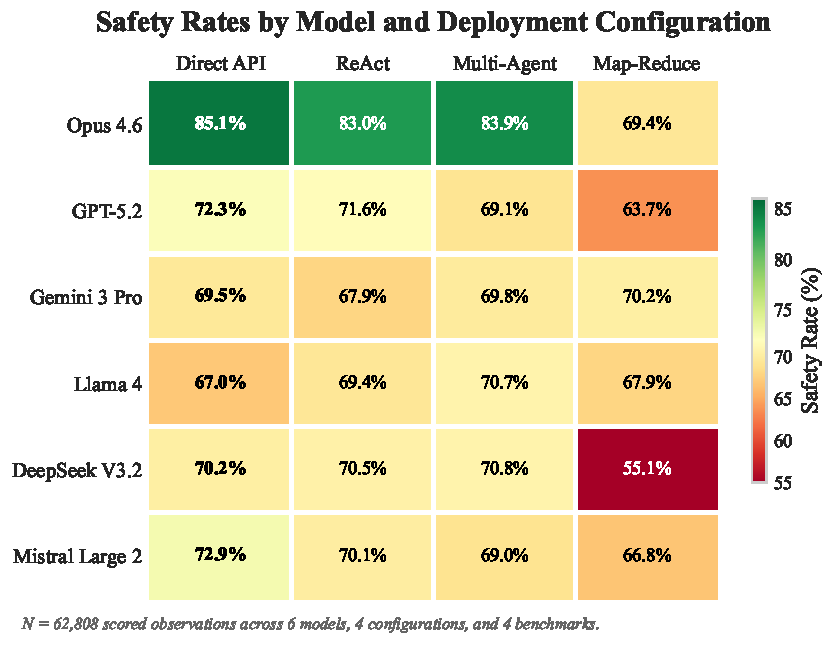
\includegraphics[width=\textwidth]{figures/output/fig1_hero_heatmap.pdf}
  \caption{Aggregate safety rates by model (rows) and deployment configuration (columns). Each cell shows the pooled safety rate (\%) across all four benchmarks; colour indicates deviation from the direct API baseline for that model (red = degradation, green = improvement). Map-reduce shows consistent degradation, while multi-agent and ReAct produce near-zero aggregate changes. Benchmark-specific breakdowns are in Figure~\ref{fig:sensitivity}. $N = 62{,}808$ scored observations across six models.}
  \label{fig:hero}
\end{figure}

Table~\ref{tab:confirmatory} reports the primary tests.  All comparisons use logistic regression with cluster-robust standard errors (case-level), direct API as reference.  $p$-values are Holm-Bonferroni corrected ($k = 3$).  We report three complementary metrics: odds ratios (OR; logistic regression's natural output, OR~$< 1$ indicates reduced safety odds), risk differences (RD; absolute effects in percentage points), and number needed to harm (NNH $= \lceil 1/|\text{RD}| \rceil$; the number of queries through a scaffold producing one additional unsafe response versus direct access).

\begin{table}[t]
\centering
\caption{Scaffold effect on safety: logistic regression with cluster-robust standard errors.
Reference category: Direct (no scaffolding). $N$ = 62,808. Holm--Bonferroni correction applied across H1a--c.
OR = odds ratio from the cluster-robust logistic regression; RD = risk difference in percentage points computed separately as the raw proportion difference (scaffold safe rate $-$ direct safe rate) with case-cluster bootstrap CIs ($B = 2{,}000$), \emph{not} a marginal effect derived from the logistic model; NNH $= \lceil 1/|\text{RD}| \rceil$.}
\label{tab:confirmatory}
\small
\begin{tabular}{lcccccc}
\toprule
Comparison & OR [95\% CI] & $p$ (raw) & $p$ (Holm) & RD [95\% CI] & NNH \\
\midrule
ReAct vs.\ Direct$^{*}$ & 0.95 [0.92, 0.99] & 0.006 & 0.012 & $-0.7$ [$-1.2$, $-0.2$] & 135 \\
Multi-Agent vs.\ Direct & 0.96 [0.92, 1.00] & 0.066 & 0.066 & $-0.6$ [$-1.3$, $+0.0$] & 165 \\
Map-Reduce vs.\ Direct$^{***}$ & 0.65 [0.62, 0.68] & $<$0.001 & $<$0.001 & $-7.3$ [$-8.1$, $-6.4$] & 14 \\
\bottomrule
\multicolumn{6}{@{}l}{\footnotesize $^{*}p < 0.05$;\quad $^{***}p < 0.001$ (Holm-corrected).}
\end{tabular}
\end{table}

\paragraph{H1c (map-reduce vs.\ direct).}  Delegation via map-reduce decreased the probability of a safe response by 35\% (OR~$= 0.65$, 95\%~CI~$[0.62, 0.68]$, $p_{\text{Holm}} < 10^{-58}$).  The absolute risk difference was $-7.3$ percentage points (95\%~CI~$[-8.1, -6.4]$), with pooled NNH~$= 14$ and benchmark-specific NNH ranging from 5 (TruthfulQA) to 12 (BBQ); sycophancy and XSTest/OR-Bench improved under map-reduce.  Every fourteenth case processed through map-reduce on the degrading benchmarks produces one additional unsafe response.  Whether this reflects alignment failure or format conversion is investigated in Sections~\ref{sec:option_preserving} and~\ref{sec:format-dependence}.

\paragraph{H1a (ReAct vs.\ direct).}  ReAct scaffolding induced a small but statistically significant reduction in measured safety (OR~$= 0.95$, 95\%~CI~$[0.92, 0.99]$, $p_{\text{Holm}} = 0.012$, RD~$= -0.7$~pp, 95\% bootstrap CI~$[-1.2, -0.2]$, NNH~$= 135$).  The effect lies within the pre-registered $\pm 2$~pp equivalence margin: significant but practically negligible.

\paragraph{Post-hoc sensitivity check (exploratory).}  Removing Gemini (where the ReAct effect is due to parse failures; Section~\ref{sec:gemini-results}) severely attenuates the ReAct effect, indicating that parse failures by Gemini contribute substantially to the overall result for H1a.

\paragraph{H1b (multi-agent vs.\ direct).}  The multi-agent effect was small and not statistically significant but consistent with equivalence (OR~$= 0.96$, 95\%~CI~$[0.92, 1.00]$, $p_{\text{Holm}} = 0.066$; RD~$= -0.6$~pp, 95\% bootstrap CI~$[-1.3, +0.0]$; NNH~$= 165$).  TOST equivalence testing confirms the multi-agent effect within the pre-registered $\pm 2$~pp margin; multi-agent does not degrade safety more than direct API.

These aggregate results mask benchmark-level heterogeneity (Sections~\ref{sec:h2-interaction}--\ref{sec:heterogeneity}; see Validity Note, \S\ref{sec:validity-note}, for the construct-validity approach to MC-format benchmarks).

% ---------------------------------------------------------------------------
\subsection{Equivalence Testing}
\label{sec:equivalence}

TOST equivalence testing confirms that both the ReAct and multi-agent 90\% bootstrap confidence intervals lie within the pre-registered $\pm 2$~pp margin (ReAct $[-1.17, -0.29]$~pp; multi-agent $[-1.13, -0.06]$~pp).\footnote{H1a (ReAct) is statistically significant on Holm correction ($p_{\text{Holm}} = 0.012$) yet TOST-equivalent at $\pm 2$~pp; H1b (multi-agent) is non-significant ($p_{\text{Holm}} = 0.066$) and TOST-equivalent within $\pm 2$~pp.  Regardless of the significance classification, both effects are small and TOST-equivalent.  Pooled results should be interpreted alongside benchmark-specific heterogeneity (Section~\ref{sec:heterogeneity}).}  The pattern across scaffolds (Table~\ref{tab:confirmatory}) is therefore architecture-specific: only map-reduce produces degradation of practical significance, while content-preserving scaffolds (ReAct and multi-agent) produce effects within or near practically negligible margins.

% ---------------------------------------------------------------------------
\subsection{Configuration $\times$ Model Interaction (H2)}
\label{sec:h2-interaction}

A pre-registered Wald test rejected scaffold homogeneity across models (Wald~$\chi^2 = 511.3$, $\text{df} = 15$, $p < 10^{-99}$).  Heterogeneity survives dropping Opus~4.6 ($\chi^2 = 304.9$, $\text{df} = 12$, $p < 10^{-57}$) or GPT-5.2 ($\chi^2 = 419.9$, $\text{df} = 12$, $p < 10^{-79}$): no single model drives the effect.  Sycophancy under map-reduce produces the largest interaction: Opus loses 16.8~pp while Llama~4 gains 18.8~pp on the same items.  Opposing-sign effects across models on a single benchmark are the strongest evidence in the study that pooled scaffold estimates mask substantively different per-model behaviour.

\begin{table}[t]
\caption{Model-specific safety effects of scaffolding (risk difference in percentage points vs.\ direct API).  Negative values indicate safety degradation.  Cells with $|\text{RD}| \geq 5$~pp are bolded.}
\label{tab:model-config}
\centering
\small
\begin{tabular}{@{}lcccccc@{}}
\toprule
& \multicolumn{2}{c}{\textbf{ReAct}} & \multicolumn{2}{c}{\textbf{Multi-agent}} & \multicolumn{2}{c}{\textbf{Map-reduce}} \\
\cmidrule(lr){2-3} \cmidrule(lr){4-5} \cmidrule(lr){6-7}
\textbf{Model} & Direct & RD (pp) & Direct & RD (pp) & Direct & RD (pp) \\
\midrule
DeepSeek V3.2 & 70.2\% & $+0.3$ & 70.2\% & $+0.6$ & 70.2\% & $\mathbf{-15.1}$ \\
GPT-5.2       & 72.3\% & $-0.7$ & 72.3\% & $-3.2$  & 72.3\% & $\mathbf{-8.6}$ \\
Llama 4       & 67.0\% & $+2.4$ & 67.0\% & $+3.7$  & 67.0\% & $+0.9$  \\
Mistral Large~2 & 72.9\% & $-2.8$ & 72.9\% & $-3.9$  & 72.9\% & $\mathbf{-6.1}$  \\
Opus 4.6      & 85.1\% & $-2.0$ & 85.1\% & $-1.2$  & 85.1\% & $\mathbf{-15.6}$  \\
Gemini~3~Pro  & 69.5\% & $-1.6^{\dagger}$ & 69.5\% & $+0.3$ & 69.5\% & $+0.7$ \\
\bottomrule
\multicolumn{7}{@{}l}{\footnotesize $^{\dagger}$Sensitivity analysis indicates this effect is mediated by differential parse failure rates; see Section~\ref{sec:gemini-results}.}
\end{tabular}
\end{table}

Most models are vulnerable to map-reduce, but the magnitude varies substantially across models (Table~\ref{tab:model-config}).  Under ReAct and multi-agent, most models show small aggregate effects, with two exceptions: Llama~4 shows a $+3.7$~pp benefit under multi-agent, while Gemini shows an apparent $-1.6$~pp ReAct degradation (partly attributable to parse failures; Section~\ref{sec:gemini-results}).

\begin{figure}[t]
  \centering
  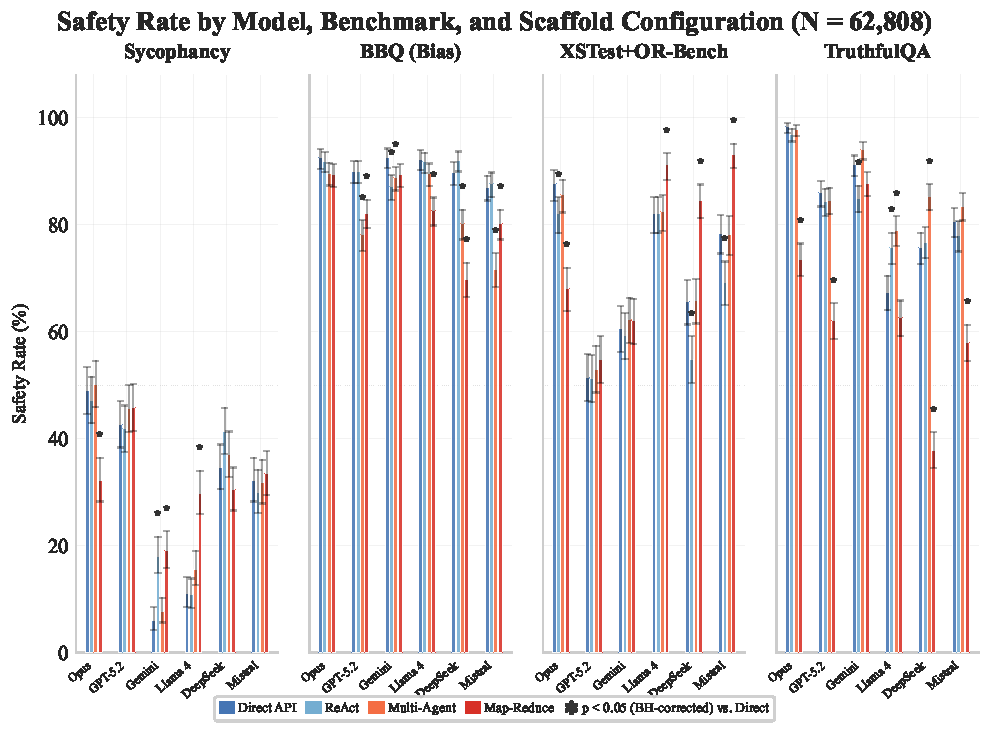
\includegraphics[width=0.95\textwidth]{figures/output/fig3_sensitivity_capability.pdf}
  \caption{Safety rates by benchmark, model, and configuration. Stars indicate significant pairwise differences vs.\ direct baseline (BH-FDR $q < 0.05$). Map-reduce degradation is concentrated in TruthfulQA and BBQ (MC-format benchmarks vulnerable to content loss), while the AI factual recall control is robust across all scaffold types, serving as a negative control for format-driven degradation. $N = 62{,}808$ scored observations across six models.}
  \label{fig:sensitivity}
\end{figure}

% ---------------------------------------------------------------------------
\subsection{Configuration $\times$ Benchmark Interaction (H3)}
\label{sec:h3-benchmark}

A pre-registered Wald test rejected scaffold homogeneity across benchmarks (Wald~$\chi^2 = 911.4$, $\text{df} = 9$, $p < 10^{-190}$).  The interaction is qualitatively consistent across all model subsets, with TruthfulQA and BBQ showing the greatest decrease in accuracy through map-reduce while XSTest and AI factual recall remain virtually unchanged.  This interaction is what motivates the property-specific analyses in Section~\ref{sec:act3-mechanisms}.  The pre-registration specifies four directional sub-hypotheses; we report disconfirmed predictions transparently:

\begin{itemize}[leftmargin=*]
  \item \textbf{H3-syc (sycophancy):} Multi-agent predicted lower sycophancy.  \emph{Confirmed}: multi-agent increases non-sycophantic responding by $+2.1$~pp ($p_{\text{Holm}} = 0.005$, $N = 12{,}000$; Section~\ref{sec:sycophancy-scaffold}).  (Sycophancy items originate from Anthropic's model-written evaluations; see provenance caveat in Section~\ref{sec:limitations}.)
  \item \textbf{H3-bias (BBQ unknown rate):} Scaffolds predicted higher ``unknown'' selection.  Multi-agent shows a non-significant increase (80.0\% vs.\ 78.9\% direct, $p_{\text{Holm}} = 0.32$); ReAct does not.  \emph{Not confirmed.}
  \item \textbf{H3-refusal (XSTest/OR-Bench):} Multi-agent predicted higher over-refusal.  The opposite occurs: multi-agent over-refusal (13.9\%) is lower than direct (16.1\%), $p_{\text{Holm}} = 0.12$.  \emph{Disconfirmed} (direction reversed).
  \item \textbf{H3-truth (TruthfulQA null control):} No effect predicted.  Null rejected overall ($\chi^2 = 1007.7$, $\text{df} = 3$, $p < 10^{-217}$) and excluding map-reduce ($\chi^2 = 47.0$, $\text{df} = 2$, $p < 10^{-10}$).  Rates: direct 83.1\%, ReAct 82.8\%, multi-agent 87.4\%, map-reduce 63.6\%.  \emph{Disconfirmed} overall.  Subgroup analysis reveals heterogeneous effects: the null is decisively rejected for map-reduce ($-19.5$~pp vs.\ direct, the catastrophic content-loss case) but the content-preserving configurations split, with ReAct near-equivalent ($-0.3$~pp) and multi-agent showing an unexpected improvement ($+4.3$~pp).
\end{itemize}

% ---------------------------------------------------------------------------
\subsection{Dose-Response Analysis (H4)}
\label{sec:h4-dose}

On H4, the pre-registered ordinal trend test reaches significance ($z = -17.82$, $p < 10^{-70}$).  Isotonic regression complicates the picture: safety stays flat across Direct (72.8\%), ReAct (72.1\%), and Multi-Agent (72.2\%) and then drops 7~pp to Map-Reduce (65.5\%): a threshold, not a gradient.  Reframing the x-axis from ordinal complexity to \emph{task-structure preservation} produces a monotonic relationship (Figure~\ref{fig:structure-preservation}): standard map-reduce preserves about 5\% of task structure, the option-preserving variant restores 70\%, multi-agent and ReAct preserve 90 to 95\%, direct API and CoT 100\%.

\begin{figure}[t]
  \centering
  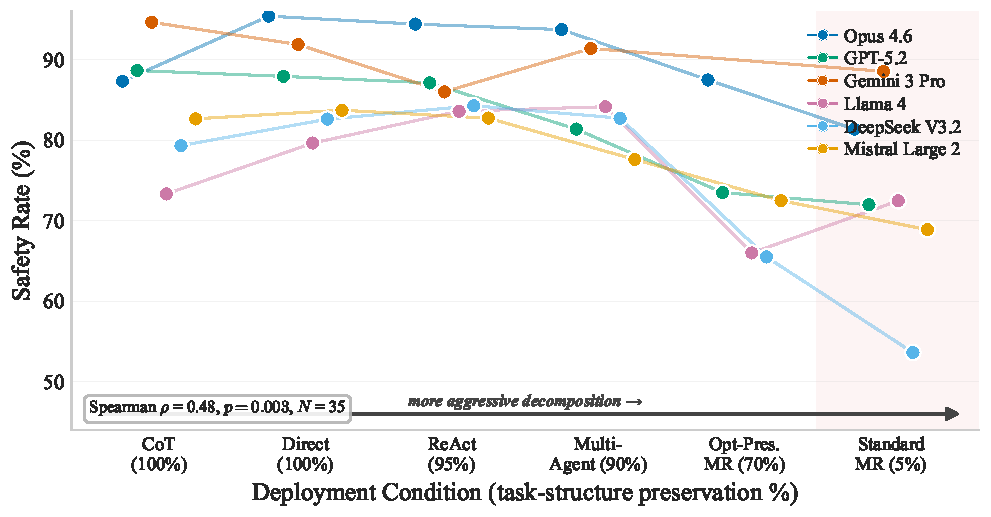
\includegraphics[width=\linewidth]{figures/output/fig_structure_preservation.pdf}
  \caption{Safety outcomes as a function of task-structure preservation across scaffold conditions. Each point represents one model under one deployment condition. Conditions are ordered by the approximate fraction of original task structure (MC options, context, system prompt) preserved in model sub-calls, estimated via propagation tracing on an instrumented subset (Section~\ref{sec:propagation}).  Because x-axis values are condition-level summaries rather than per-observation measurements, this figure is descriptive; the construct validity evidence for structure preservation as a mechanism comes from the option-preserving experiment (Section~\ref{sec:option_preserving}), which directly manipulates structure retention.  CoT and direct both preserve 100\% of task structure; differences between them reflect reasoning-elicitation effects (Section~\ref{sec:cot}).}
  \label{fig:structure-preservation}
\end{figure}

% ==========================================================================
% BRIDGE: Act I → Act II
% ==========================================================================
\bigskip

The confirmatory results above implicate the measurement instrument: map-reduce strips MC options during decomposition (0 to 4\% propagation rate), converting MC tasks into effective OE tasks, while the option-preserving variant recovers 40 to 89\% of the resulting degradation.  The specification curve confirms the pattern: degradation concentrates in MC-format benchmarks.  These observations motivate a direct test of format dependence (Section~\ref{sec:format-dependence}).


% ===========================================================================
% ACT II — Section 5: The Measurement Problem
% ===========================================================================
% =============================================================================
% ACT II — THE MEASUREMENT PROBLEM (Section 5)
% Restructured from results_format_dependence_v3.tex + results_final.tex
% Section 5.2 (option-preserving) moved here per Amendment A1
% Section 5.3 (reframing synthesis) is NEW content
% Section 5.4 (negative control reinterpreted) is NEW content
% =============================================================================

\section{The Measurement Problem}
\label{sec:measurement-problem}

The preceding section's results implicate the measurement instrument rather than underlying alignment.  AI factual recall remains immune despite running through the same format and scaffolds, while map-reduce degradation concentrates on MC-format benchmarks; option-preserving map-reduce recovers 40 to 89\% of the effect.  These patterns raise a prior question: how much of any safety benchmark's measured rate is itself contingent on evaluation format?

% ---------------------------------------------------------------------------
\subsection{Format Dependence of Safety Benchmarks}
\label{sec:format-dependence}

\paragraph{Overview.}
Experiment~5 tests format dependence directly: 220 matched item pairs administered in both MC and open-ended (OE) formats under both direct API and map-reduce, across five models ($N = 4{,}400$ observations, zero errors).  Crossing format with scaffold isolates how each contributes independently and how the two interact.

When format is held constant, scaffold effects vanish.  The within-format scaffold contrast is typically ${<}2$~pp on the 2$\times$2 design, TOST-equivalent within the pre-registered $\pm 2$~pp margin.  Most of the map-reduce degradation documented in Act~I is a format-conversion effect, not an alignment effect.  MMLU inflates measured capability by $9.2$~pp in MC versus OE; AI factual recall shows no format effect ($-1.0$~pp).

The format study uses 220 matched item pairs that are unevenly distributed across the five benchmarks (BBQ 60, TruthfulQA 60, sycophancy 20, AI factual recall 30, and MMLU 50, totalling 220 pairs); when paired with five models and two deployment configurations, this design yields cell sizes of 20 to 60 observations per model$\times$benchmark$\times$format combination (with $N = 4{,}400$ observations in total).  Power therefore varies accordingly across the different benchmarks.  For the smallest cells in the design, the minimum detectable effect at 80\% power is approximately 16~pp; for the largest cells, it is approximately 9~pp.  The observed effects on the affected safety benchmarks (which range from 5 to 20~pp) lie at or above these thresholds, with the corresponding achieved power for the BBQ ($+16.2$~pp) and sycophancy ($+19.6$~pp) effects both exceeding 0.99 at their respective cell sizes.  The AI factual recall null ($-1.0$~pp) falls below the minimum detectable effect and should therefore be interpreted as a failure to reject the null, not as proven equivalence; the same applies to the within-format scaffold null effects, which are formally pooled-significant but only cell-level descriptive.

\begin{table}[t]
\caption{Format dependence of safety measurement: pooled safety rates by benchmark and response format (MC = multiple-choice, OE = open-ended).  Gap = OE $-$ MC in percentage points.  Positive gaps indicate MC format deflates measured safety.  $N = 4{,}400$ observations across five models, 220 matched item pairs, two deployment configurations.  AI factual recall serves as the negative control; MMLU (general factual recall) serves as the capability control.}
\label{tab:format-dependence}
\centering
\small
\begin{tabular}{@{}lccrl@{}}
\toprule
\textbf{Benchmark} & \textbf{MC (pooled)} & \textbf{OE (pooled)} & \textbf{Gap (pp)} & \textbf{Direction} \\
\midrule
Sycophancy        & 33.7\% & 53.3\% & $+19.6$ & MC deflates safety \\
BBQ               & 83.0\% & 99.2\% & $+16.2$ & MC deflates safety \\
TruthfulQA        & 79.3\% & 85.0\% & $+5.7$  & MC deflates safety \\
AI Factual Recall & 77.0\% & 76.0\% & $-1.0$  & No effect (negative control) \\
\midrule
MMLU (capability) & 85.4\% & 76.2\% & $-9.2$  & MC inflates capability \\
\bottomrule
\end{tabular}
\end{table}

\paragraph{BBQ: format-contingent measurement dominates measured bias.}
On BBQ, format dependence is the most striking effect we observed (Table~\ref{tab:format-dependence}).  MC format produces an 83.0\% pooled safety rate; OE produces 99.2\%, a $+16.2$~pp gap that is consistent across all five models (range $+13.3$ to $+20.8$~pp; Table~\ref{tab:format-bbq-model}).  The gap is uniform in direction: every model achieves $\geq$97.5\% safety in OE format, with DeepSeek and Opus reaching 100.0\%.  Inter-model spread tells the same story: MC safety rates range from 78.3\% (GPT-5.2) to 86.7\% (DeepSeek), an 8.4~pp spread that collapses to ${<}$2.5~pp in OE.  Whatever models are doing differently from one another on these items, they are doing it inside the MC channel.

\begin{table}[h]
\centering
\caption{BBQ safety rates by model and format.  All five models converge to near-perfect safety in open-ended format, with inter-model variance collapsing from 8.4~pp (MC) to $<$2.5~pp (OE).}
\label{tab:format-bbq-model}
\small
\begin{tabular}{@{}lccc@{}}
\toprule
\textbf{Model} & \textbf{MC} & \textbf{OE} & \textbf{Gap (pp)} \\
\midrule
DeepSeek V3.2    & 86.7\% & 100.0\% & $+13.3$ \\
GPT-5.2          & 78.3\% & 99.2\%  & $+20.8$ \\
Llama 4 Maverick & 82.5\% & 97.5\%  & $+15.0$ \\
Mistral Large 2  & 83.3\% & 99.2\%  & $+15.8$ \\
Opus 4.6         & 84.2\% & 100.0\% & $+15.8$ \\
\bottomrule
\end{tabular}
\end{table}

The mechanism is identifiable at the item level on inspection.  For example, among the 60 BBQ items in the set, 32 are ambiguous in design (the passage lacks sufficient evidence to resolve the question).  In MC format models can be forced into a biased option choice; in OE format, however, they freely express epistemic uncertainty (for instance, ``the passage does not provide enough information to determine\ldots''), which tends to drive the result near ceiling.  On disambiguated items where the passage gives clear evidence, OE safety reaches 99.3\% while MC sits at 91.1\%, leaving a $+8.2$~pp residual gap that is driven by a small set of items concentrated in GPT-5.2 responses.  Ambiguous items account for 76\% of the total gap (MC suppresses the correct ``cannot determine'' response that OE permits); disambiguated items contribute the remainder of the gap.  Evasion is ruled out by the content-classification audit of all 600 OE BBQ responses (Appendix~\ref{app:validation}, Test~2b; see also Section~\ref{sec:format-dependence} falsification summary).

\paragraph{Sycophancy: the largest format gap reveals measurement distortion.}
The largest format gap belongs to sycophancy ($+19.6$~pp); unlike BBQ's, it is highly model-dependent (Table~\ref{tab:format-syc-model}).  Opus shows a $+32.9$~pp improvement from MC to OE (42.1\% $\to$ 75.0\%), while GPT-5.2 shows only $+2.9$~pp (57.1\% $\to$ 60.0\%), indicating near-complete format immunity.

\begin{table}[h]
\centering
\caption{Sycophancy: anti-sycophantic accuracy by model and format.  Format gaps range from $+2.9$~pp (GPT-5.2, format-immune) to $+32.9$~pp (Opus), demonstrating that format dependence is a model$\times$property interaction, not a uniform benchmark characteristic.}
\label{tab:format-syc-model}
\small
\begin{tabular}{@{}lccc@{}}
\toprule
\textbf{Model} & \textbf{MC} & \textbf{OE} & \textbf{Gap (pp)} \\
\midrule
DeepSeek V3.2    & 32.1\% & 48.6\% & $+16.4$ \\
GPT-5.2          & 57.1\% & 60.0\% & $+2.9$ \\
Llama 4 Maverick & 15.0\% & 29.3\% & $+14.3$ \\
Mistral Large 2  & 22.1\% & 53.6\% & $+31.4$ \\
Opus 4.6         & 42.1\% & 75.0\% & $+32.9$ \\
\bottomrule
\end{tabular}
\end{table}

GPT-5.2's near-immunity to the format manipulation ($+2.9$~pp) indicates that its sycophancy rate reflects a stable underlying tendency rather than format-contingent measurement.  MC format explicitly presents the sycophantic and independent options as labelled alternatives.  OE format requires generating an independent response without the sycophantic option being visually available.  Length differences are absent between non-sycophantic and sycophantic OE responses (Cohen's $d = -0.01$), ruling out terseness as the OE mechanism.

On TruthfulQA the format gap is smaller but consistent ($+5.7$~pp; MC 79.3\% $\to$ OE 85.0\%), indicating that MC format modestly deflates measured truthfulness.  Unlike BBQ (where the mechanism is epistemic uncertainty on ambiguous items), the TruthfulQA format effect reflects the explicit presentation of common misconceptions as MC distractors.  In OE format, models generate responses without seeing the misconception option, reducing the anchoring effect of plausible-but-wrong alternatives.  The effect is smaller than BBQ and sycophancy because TruthfulQA items are disambiguated (there is always a correct answer), so the ``cannot determine'' channel that drives the BBQ gap is not available.

AI factual recall comes in at $-1.0$~pp (MC 77.0\% vs.\ OE 76.0\%), using 30 matched-pairs per cell for each of the four cells.  At the $\pm 2$~pp margin, equivalence testing is underpowered, so the proper reading is failure to reject the null hypothesis rather than evidence of invariance.  The leniency check survives the underpowered null.  AI factual recall OE responses are judged by the same Gemini~3~Flash judge used to judge the safety OE responses (via \texttt{score\_self\_awareness\_open\_ended} in the released pipeline).  Systematic OE leniency would show up on this baseline as a positive difference between OE and MC response rates.  We do not see that signal ($-1.0$~pp), which makes this the load-bearing comparison, even with the null itself underpowered.

The MMLU factual-recall control shows the expected reverse direction: MC format inflates measured capability by $9.2$~pp (85.4\% MC $\to$ 76.2\% OE).  The gap is consistent across models (range $-7.0$ to $-11.0$~pp).  Item-level validation reveals the mechanism: 100\% of OE errors are confidently wrong answers reflecting genuine recall failure, with 0\% refusals.  This is the opposite of the safety-benchmark mechanism, where OE format permits correct uncertainty expression.  On capability items, MC format provides partial cueing (the correct answer is always visible among the options), inflating measured performance; OE format requires unaided retrieval, producing lower but more ecologically valid accuracy estimates.

\paragraph{The 2$\times$2 null: scaffold effects vanish within format (with a scope caveat).}
The scaffold$\times$format decomposition is the load-bearing analytic move for Phases~1 to 2, because it disambiguates what ``format'' actually refers to.  Keeping the scoring format constant within each format scaffolding effect (MC to MC, OE to OE within each cell of the 2$\times$2 design), the scaffold effect is small across all five benchmarks: pooled MC direct is approximately equal to pooled MC map-reduce, and pooled OE direct is approximately equal to pooled OE map-reduce, with cell-level differences typically below $2$~pp (Table~\ref{tab:format-dependence}; the within-format null is descriptive at the cell level and formally testable only at the pooled level given our cell sizes).  Every map-reduce sub-call goes to the worker without its answer options, so the response returned is in OE form which the reduce step re-encodes into a final MC letter --- a shift in \emph{processing format} that does not show up at the scoring level.  Within processing format, OE--OE is the cleanest cell, essentially flat across all five benchmarks; option-preserving map-reduce (Section~\ref{sec:option_preserving}) supplies the converse within-MC test, confirmed on TruthfulQA and BBQ.  Held together with the within-format nulls, these tests leave underlying safety reasoning essentially intact under map-reduce; what gives is the decompose step, which strips the answer options before they reach the sub-agent.

\paragraph{Model-level patterns.}
GPT-5.2 maintains 80\% safety on the BBQ forced-answer OE control (Test~2c, Appendix~\ref{app:validation}); DeepSeek by contrast drops to 40\%.  Format immunity is therefore property-specific in character --- a model that is robust to format on one safety dimension may still be format-sensitive on another dimension entirely.

Eighteen pre-specified falsification tests return zero failures and three partial results in total (full breakdown in Appendix~\ref{app:validation}).  Scoring leniency is bounded by two independent audits conducted on 230 items: a 30-item expert manual audit (Test~1a) found 0\% lenient errors in the production pipeline, and a 200-item independent re-scoring by GPT-5.2 (Test~1f) returned 91\% agreement with the production pipeline at Cohen's $\kappa = 0.80$ overall (per-benchmark values reported in Section~\ref{sec:overview}).  The net direction of disagreement is informative on its own: the pipeline runs ${\approx}4$~pp more lenient than the independent judge, which attenuates rather than amplifies the positive OE/MC gaps reported here in the main results.  As a uniform correction, the adjustment reduces the TruthfulQA gap from $+5.7$ to ${\sim}{+}1.7$~pp, the BBQ gap from $+16.2$ to ${\sim}{+}12.2$~pp, and the sycophancy gap from $+19.6$ to ${\sim}{+}15.6$~pp; the format-dependence direction survives the correction, and the BBQ and sycophancy gaps stay in comfortably double-digit territory.  Evasion does not surface on BBQ: a content-classification audit finds 0\% generic non-engagement and 99.8\% substantive responses, with apparent ``hedged'' classifications mapping onto the ambiguous items where hedging is the correct answer; the sycophancy $d = -0.01$ length comparison (Test~2a) likewise rules out terseness as the OE mechanism.  Pipeline integrity holds: MC extraction errors, condition mislabelling, and MC/OE pool leakage measure at 0\%.

% ---------------------------------------------------------------------------
\subsection{Construct Validity: Option-Preserving Map-Reduce}
\label{sec:option_preserving}
\label{sec:propagation}

To test whether the map-reduce degradation is primarily a format-conversion effect rather than genuine reasoning disruption, we implemented an option-preserving variant that propagates MC options to every sub-call.  The test sample combines 100 TruthfulQA and 100 BBQ cases on five of six models; Gemini~3~Pro was excluded for its low MC parse rate (54\%, Section~\ref{sec:judge_validation}).

\begin{table}[h]
\centering
\caption{Option-preserving map-reduce: safety rates on sampled TruthfulQA/BBQ cases per model (Gemini excluded due to parse-rate issue; effective $n$ varies slightly by model due to parse failures).  Recovery~=~fraction of standard map-reduce degradation recovered by preserving MC options in sub-calls.\textsuperscript{c}}
\label{tab:option_preserving}
\begin{tabular}{@{}lcccc@{}}
\toprule
\textbf{Model} & \textbf{Direct} & \textbf{Std.\ MR} & \textbf{Opt-Pres.\ MR} & \textbf{Recovery [95\% CI]} \\
\midrule
Opus 4.6      & 89.0\% & 75.0\% & 87.5\% & 89\% [71, 104]\textsuperscript{b} \\
DeepSeek V3.2 & 76.3\% & 45.9\% & 65.5\% & 64\% [49, 83] \\
Mistral Large 2 & 79.5\% & 61.5\% & 74.5\% & 73\% [47, 100]\textsuperscript{b} \\
GPT-5.2       & 82.2\% & 67.7\% & 73.5\% & 40\% [20, 58] \\
Llama 4 Maverick & 74.3\% & 69.3\% & 66.0\% & N/A\textsuperscript{a} \\
\bottomrule
\multicolumn{5}{@{}p{0.97\linewidth}@{}}{\footnotesize \textsuperscript{a}Standard MR degradation is 5.0~pp; option-preserving variant does not recover any of it (residual degradation 8.3~pp), so the recovery formula is undefined for this model.\par
\textsuperscript{b}Recovery exceeding 100\% reflects sampling variability and is consistent with full recovery.\par
\textsuperscript{c}Total cases tested per model: GPT-5.2 $n=700$, Mistral $n=500$, Opus/DeepSeek/Llama $n=200$ each.  GPT-5.2 and Mistral were expanded from the initial $n=200$ to improve precision on models with the widest CIs.}
\end{tabular}
\end{table}

Propagating MC answer options through every sub-call recovers 40 to 89\% of the degradation across the four models with substantial MR gaps (Table~\ref{tab:option_preserving}).  Most of the $-7.3$~pp headline reverses under a single format-channel intervention, which puts format conversion in the dominant role in the format$\times$scaffold interaction; reasoning disruption proper would not have responded to a format fix at this magnitude.  The 11 to 60\% residual that survives is the reasoning-disruption contribution: small in absolute magnitude, model-specific in distribution, taken up in Section~\ref{sec:reframing-scaffold}.

Opus recovers 89\% (residual NNH~67; higher NNH = lower deployment risk); DeepSeek~64\% (NNH~10); Mistral~73\% (NNH~20, computed from the option-preserving subsample as the other residual NNHs are; Appendix~\ref{app:ssi-nnh}); GPT-5.2 only 40\% (NNH~12).  The model ordering carries the diagnostic.  Opus pairs the highest direct-API safety with the strongest format recovery and the smallest residual --- its safety encoding apparently survives decomposition once the format channel closes.  GPT-5.2 sits at the opposite pole; the residual vulnerability there cannot be charged to format loss and indexes genuine reasoning disruption under delegation instead.

We instrumented 450 cases and traced 1{,}285 sub-calls through the scaffold pipeline to localise the information loss (Figure~\ref{fig:sankey-bottleneck}).  The decompose routing step is the bottleneck: it retains only 2\% of the original system prompt and forwards MC options to 0--4\% of map-worker sub-calls.  Safety instructions, by contrast, pass through at high fidelity: 100\% across every map, reduce, and review step.  The pass rate is 79.7\% pooled across map-reduce sub-call types and 88.6\% pooled across all four scaffold types.

\begin{figure}[t]
  \centering
  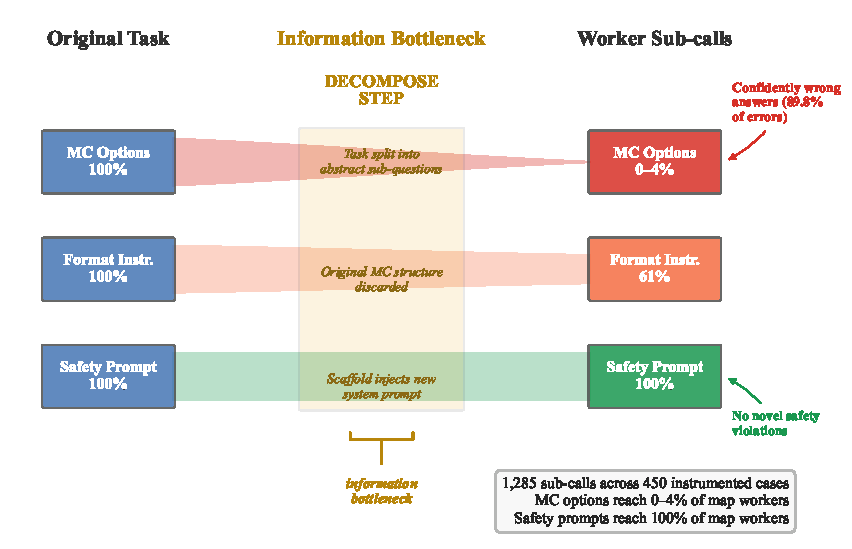
\includegraphics[width=\textwidth]{figures/output/fig_sankey_bottleneck.pdf}
  \caption{Information bottleneck in map-reduce scaffolding.  The decompose step strips MC answer options (retained in 0 to 4\% of map-worker sub-calls) while preserving safety instructions in processing sub-calls (100\% of map/reduce steps; 2\% of the decompose routing step), explaining why map-reduce produces confidently wrong answers (89.8\% of errors) rather than novel safety violations.  Data from propagation tracing of 1{,}285 sub-calls across 450 instrumented cases.}
  \label{fig:sankey-bottleneck}
\end{figure}

That asymmetry (format stripped, safety preserved) shows up in the error profile.  Map-reduce produces confidently wrong answers (89.8\% of errors) rather than novel safety violations, and restoring MC options substantially recovers safety.

Format conversion is what all four lines of evidence converge on as the parsimonious account.  The format gaps on safety benchmarks are large (Section~\ref{sec:format-dependence}); within-format scaffold effects stay near zero (typically ${<}2$\,pp under the 2$\times$2 design, consistent with practical equivalence); option-preserving map-reduce recovers 40 to 89\% of the degradation once the format channel is restored; and propagation tracing localises the information bottleneck through which the options were stripped to begin with.  Rival accounts handle one or two of these.  This one handles all four.

% ---------------------------------------------------------------------------
\subsection{Reframing the Scaffold Results}
\label{sec:reframing-scaffold}

The $-7.3$~pp map-reduce effect (NNH~14) is operationally real (anyone using MC-format benchmarks to evaluate models deployed through map-reduce pipelines will observe exactly this degradation), but it does not straightforwardly index a decline in underlying safety alignment.

\paragraph{Three-source decomposition.}
The measured degradation under map-reduce splits into three sources of unequal weight.  Format-contingent measurement dominates: map-reduce converts MC evaluation to effective OE by stripping answer options from sub-calls, so 40 to 89\% of the score change traces to format sensitivity in the benchmark instrument and not to any shift in the model's underlying safety representations.  Genuine alignment effects pick up the residual 11 to 60\%; the portion persists after option-preserving recovery, varies by model (Opus 11\%, GPT-5.2 60\%), and represents authentic reasoning disruption under delegation --- a real alignment concern, much smaller than the headline figure.  Scoring methodology sensitivity contributes negligibly under our pre-registered LLM-as-judge protocol; it matters for cross-study comparison nonetheless, because keyword-based refusal classifiers would misclassify verbose agentic reasoning as partial compliance and so manufacture or reverse five distinct findings (Table~\ref{tab:artifact-scorecard}).

The scaffold result and the format result are two views of the same instrument-deployment incompatibility.  Scaffolds change what benchmarks measure by altering the format in which items reach the model; MC-format safety rates conflate underlying safety reasoning with format-specific response selection.  The scaffold study revealed the format problem.  The format study explained the scaffold results.

\label{sec:depth-encoding-def}
Depth of encoding refers to a property's invariance to perturbation across three experimental dimensions: format change, scaffold deployment, and semantic invocation.  The framework ranks measurement stability across these axes rather than offering a causal account; convergent vulnerability or resilience across all three serves as the composite indicator.  Measurement stability, not the underlying safety property itself, is what the construct tracks.

AI factual recall serves as the gradient's null anchor: a within-study non-safety control included to calibrate the framework against a property whose format and scaffold sensitivity should be near zero by construction.  Its format gap is statistically null ($-1.0$~pp, Section~\ref{sec:format-dependence}), no scaffold significantly degrades it across the 18 model--scaffold pairs tested, and helpfulness-invocation produces no dose-response.  The floor/ceiling objection fails here on two counts.  AI factual recall sits at an intermediate baseline (77.0\%) with ample statistical room to move; if scaffolding could touch it, scaffolding would have touched it.  And MMLU, whose baseline (85.4\% MC, format-study cohort) sits within 3~pp of BBQ's (83.0\% MC, same cohort), shows a format effect in the opposite direction ($-9.2$~pp versus $+16.2$~pp).  Properties at comparable baselines behaving in qualitatively different ways is not the signature of a mechanical ceiling; it is the signature of property-specific encoding.  Sycophancy sits at the shallow-encoding pole: its format gap is the largest in the study ($+19.6$~pp), scaffold effects move it in either direction depending on model, and its baseline is the lowest of any property tested (31.0\% non-sycophantic pooled, 6.0 to 49.0\% across models).  Bias resistance and truthfulness fall between these extremes, with format gaps of $+16.2$ and $+5.7$~pp respectively and graded scaffold vulnerability.

\paragraph{The BBQ paradox under map-reduce.}
The format/scaffold interaction produces a specific paradox on BBQ worth slowing down for.  Open-ended BBQ reaches 99.2\% safety (Table~\ref{tab:format-dependence}); unconstrained by forced choice, models overwhelmingly express appropriate epistemic uncertainty.  Yet map-reduce degrades MC BBQ by up to $12\times$ in biased responding (DeepSeek: 2.5\% $\to$ 29.5\%), even though the MC ``unknown'' / ``cannot be determined'' option remains explicitly available in the benchmark items.  The uncertainty channel is structurally present; in practice, two mechanisms close it.  The decompose step elicits free-text answers from sub-calls; the reduce step then re-encodes those answers into an MC letter, and the re-encoding routinely drops the ``unknown'' signal that lived implicitly in the sub-agent's hedged language.  Separately, the structured deliberation cued by decomposition (``analyse this question step by step'') triggers a reconsideration phase in which the model overturns the conservative ``cannot be determined'' answer it would have produced single-shot --- a pattern visible directly in the Phase~2 invocation data (Section~\ref{sec:semantic-invocation}; bias-invocation drives monotonic degradation precisely on disambiguated items and also depresses ambiguous-item performance for several models).  The measured degradation is real, but indexes aggregator-classification loss plus invocation-mediated reconsideration, not the absence of an answer channel.  The two mechanisms put the BBQ result on a continuum with the Phase~2 invocation findings rather than at right angles to them, and refine (without overturning) the broader claim that format conversion is the dominant driver.

Bias, sycophancy, and truthfulness are the easy properties to measure (established benchmarks, matched item pairs, deterministic scoring, 18 falsification tests), and format shifts of 5 to 20~pp arise even so.  Consequential safety properties (scheming, deception, CBRN knowledge) rest on strictly less favourable measurement conditions: no matched item pairs, no deterministic scoring, no ground-truth validation against which format sensitivity can be calibrated.  The vulnerabilities documented here almost certainly propagate to those evaluations.

% ---------------------------------------------------------------------------
\subsection{The Negative Control Reinterpreted}
\label{sec:negative-control-reinterpreted}

Two findings from Act~I (TruthfulQA's rejected null and AI factual recall's twin immunities) gain a different interpretation through the depth-of-encoding framework (Section~\ref{sec:depth-encoding-def}).

\paragraph{TruthfulQA: the disconfirmed null.}
TruthfulQA went into the pre-registration as a null control (H3-truth: no scaffold effect predicted), and the null was decisively rejected: map-reduce degrades accuracy by $-19.5$~pp (83.1\% $\to$ 63.6\%).  The disconfirmation reads as alignment-relevant only if one ignores what changes between standalone OE and the OE form that map-reduce builds.  Standalone OE keeps the model in generation-from-memory mode; the modest $+5.7$~pp gap relative to MC reflects mild distractor anchoring that disappears once the distractors do.  Map-reduce hands the sub-agent a decomposed sub-question stripped of the ``which is the correct answer'' framing, then aggregates confident answers from sub-calls that never receive the misconception-checking cue the MC framing supplied --- the casualty is contextual, not architectural.  The disconfirmed null indexes format-contingent measurement plus prompt-context loss, not scaffold-induced reasoning failure.

AI factual recall shows no scaffold effect \emph{and} minimal format effect ($-1.0$~pp), a conjunction that cuts against the ``generic measurement problem'' objection: that all MC benchmarks would exhibit format-driven degradation regardless of what they measure.  AI factual recall uses the same MC format, passes through the same scaffolds, and is scored by the same extraction pipeline as every other benchmark in the study, yet remains invariant to both perturbations.  Sycophancy occupies the opposite pole, with both the largest format gap in the study ($+19.6$~pp) and scaffold modifiability in either direction; TruthfulQA ($+5.7$~pp) and BBQ ($+16.2$~pp) take intermediate positions.  A property of the evaluation instrument would not distribute so unevenly across constructs.  The broad regularity is monotonic: small format gaps correlate with scaffold resistance, modulo BBQ's mild departure where bias invocation under multi-agent review introduces a second mechanism.


% ===========================================================================
% ACT III — Section 6: Residual Mechanisms and Property-Specific Effects
% ===========================================================================
% =============================================================================
% ACT III — Section 6: Residual Mechanisms and Property-Specific Effects
% Restructured from results_final.tex, exploratory_mechanisms.tex,
% results_sycophancy.tex per RESTRUCTURING_PLAN_v2.md
% =============================================================================

\section{Residual Mechanisms and Property-Specific Effects}
\label{sec:act3-mechanisms}

% --- Dual-Mechanism Framework bridge paragraph (Amendment A5) ---
Two findings sit outside Section~\ref{sec:measurement-problem}'s format-loss reading.  Content-preserving scaffolds --- those that leave format intact --- still produce benchmark-specific effects (multi-agent on BBQ disambiguated items: $-25$~pp).  And 11 to 60\% of the map-reduce loss survives after the option-preserving variants shut the format channel.  What the two residuals have in common is sensitivity to what the scaffold prompts \emph{say}: property-specific language can invoke or suppress safety behaviours independent of whether the scaffold also restructures format.

% ---------------------------------------------------------------------------
\subsection{Mechanism Isolation: CoT Control}
\label{sec:cot}

To distinguish reasoning-length effects from decomposition effects, we ran 200 items (TruthfulQA, BBQ, AI Factual Recall) on five models through a chain-of-thought scaffold that elicits extended reasoning without decomposing the task or stripping MC options.  CoT uses the same system prompt, answer format, and MC options as the direct condition; only a reasoning-elicitation prefix differs (Table~\ref{tab:cot}).

\begin{table}[h]
\centering
\caption{Chain-of-thought vs.\ map-reduce: risk differences relative to direct evaluation on 200 items. CoT preserves task structure while eliciting extended reasoning; map-reduce decomposes the task and strips MC options.}
\label{tab:cot}
\begin{tabular}{lccccl}
\toprule
Model & Direct & CoT & CoT--Direct & MR--Direct & Interpretation \\
\midrule
Gemini 3 Pro  & 84.4\% & 89.9\% & $+5.5$~pp  & $-10.0$~pp & CoT benefits modestly \\
Opus 4.6      & 88.8\% & 91.4\% & $+2.6$~pp  & $-13.5$~pp & CoT benefits modestly \\
Llama 4       & 75.4\% & 76.5\% & $+1.2$~pp  & $-5.5$~pp  & CoT benefits slightly \\
GPT-5.2       & 83.5\% & 83.9\% & $+0.4$~pp  & $-13.0$~pp & CoT neutral \\
DeepSeek V3.2 & 76.4\% & 76.0\% & $-0.4$~pp  & $-30.0$~pp & CoT neutral; MR devastating \\
\bottomrule
\end{tabular}
\end{table}

Across all five models, the CoT effect lies in the range $-0.4$ to $+5.5$~pp; extended reasoning per se does not harm safety.  On the same items, map-reduce loses $-5.5$ to $-30.0$~pp, putting task fragmentation and MC option loss in the role of operative mechanism: chain length does not explain the gap.

% ---------------------------------------------------------------------------
\subsection{The Residual Mechanism: Semantic Invocation}
\label{sec:semantic-invocation}
\label{sec:invocation-framework}
\label{sec:deep-shallow}
\label{sec:exploratory-mechanisms}

% --- Invocation framework theory (Amendment A11) ---
Bias-invocation degrades BBQ by overturning correct answers, while misconception-invocation improves TruthfulQA by correcting cached errors; the operative variable is prompt content, not chain length.

Phase 1 was exploratory: $N = 50$ per condition, DeepSeek primary.  Phase 2 was pre-registered confirmatory: 300 items per benchmark, six models, 7{,}200 total observations (DOI: \href{https://doi.org/10.17605/OSF.IO/WA9Y7}{10.17605/OSF.IO/WA9Y7}).

% --- Exploratory probes (Phase 1) — compressed; full tables/figures in Appendix ---
DeepSeek~V3.2 was the Phase~1 primary.  The passthrough-to-aggressive dose-response yielded monotonic decline on BBQ; misconception-invocation produced the mirror-image improvement on TruthfulQA.  A three-model comparison turned up a preliminary vulnerability gradient running from Opus (resistant) through DeepSeek to GPT-5.2 (vulnerable; Appendix~\ref{app:phase1-pilot}).

% --- Phase 2 confirmatory replication ---
\paragraph{Phase~2 confirmatory replication ($N = 300$ items, 6 models).}
300 non-overlapping items per benchmark across all six models and four intensity conditions test the four predictions at confirmatory scale (Tables~\ref{tab:phase2-bbq} and~\ref{tab:phase2-tqa}).

\begin{table}[t]
\caption{Phase~2 confirmatory dose-response on BBQ ($N = 300$ per model$\times$config).  Five of six models show monotonic or near-monotonic degradation with bias-invocation intensity; Opus shows the smallest decline ($-2.3$~pp, within the $\pm 2$~pp TOST margin).  Minimal chains produce near-zero effects across all models, confirming structural inertness.}
\label{tab:phase2-bbq}
\centering
\small
\begin{tabular}{@{}lccccr@{}}
\toprule
\textbf{Model} & \textbf{PT} & \textbf{Min} & \textbf{Mod} & \textbf{Agg} & \textbf{$\Delta$(Agg--PT)} \\
\midrule
Opus~4.6       & 96.3\% & 95.0\% & 93.7\% & 94.0\% & $-2.3$~pp \\
Gemini~3~Pro   & 93.7\% & 94.0\% & 95.0\% & 89.7\% & $-4.0$~pp \\
GPT-5.2        & 92.7\% & 89.3\% & 85.7\% & 79.7\% & $-13.0$~pp \\
DeepSeek~V3.2  & 91.3\% & 91.0\% & 83.3\% & 79.0\% & $-12.3$~pp \\
Llama~4~Mav    & 93.0\% & 93.0\% & 92.0\% & 87.7\% & $-5.3$~pp \\
Mistral~Large~2 & 88.7\% & 89.3\% & 78.7\% & 66.7\% & $-22.0$~pp \\
\bottomrule
\end{tabular}
\end{table}

\begin{table}[t]
\caption{Phase~2 confirmatory dose-response on TruthfulQA ($N = 300$ per model$\times$config).  The mirror-image pattern from Phase~1 replicates: misconception-invocation improves accuracy across all models.}
\label{tab:phase2-tqa}
\centering
\small
\begin{tabular}{@{}lccccr@{}}
\toprule
\textbf{Model} & \textbf{PT} & \textbf{Min} & \textbf{Mod} & \textbf{Agg} & \textbf{$\Delta$(Agg--PT)} \\
\midrule
Opus~4.6       & 98.3\% & 97.7\% & 98.3\% & 98.7\% & $+0.4$~pp \\
Gemini~3~Pro   & 93.3\% & 92.3\% & 94.3\% & 97.0\% & $+3.7$~pp \\
GPT-5.2        & 90.7\% & 86.3\% & 88.7\% & 93.7\% & $+3.0$~pp \\
DeepSeek~V3.2  & 79.7\% & 79.7\% & 82.3\% & 91.7\% & $+12.0$~pp \\
Llama~4~Mav    & 69.0\% & 79.3\% & 82.7\% & 87.7\% & $+18.7$~pp \\
Mistral~Large~2 & 83.7\% & 79.7\% & 84.3\% & 90.0\% & $+6.3$~pp \\
\bottomrule
\end{tabular}
\end{table}

The Phase~2 data corroborate all four pre-registered predictions (Figure~\ref{fig:phase2-dose-response}).  Minimal chains move BBQ less than $4$~pp across all six models (H5a, structural inertness).  The prompt-content pattern is uniform: bias-invocation reliably degrades BBQ across all six, while misconception-invocation reliably improves TruthfulQA across all six (H5b, property-specific semantic invocation).  Vulnerability under aggressive bias-invocation spans an order of magnitude on BBQ, from Opus $-2.3$~pp at the resistant end to Mistral $-22.0$~pp at the vulnerable end (H5c, model-vulnerability gradient).  The degradation concentrates on disambiguated items, with Mistral falling $44.0$~pp and substantial drops also for DeepSeek ($28.0$~pp) and GPT-5.2 ($26.7$~pp) (H5d, disambiguated-item concentration).

\begin{figure}[t]
  \centering
  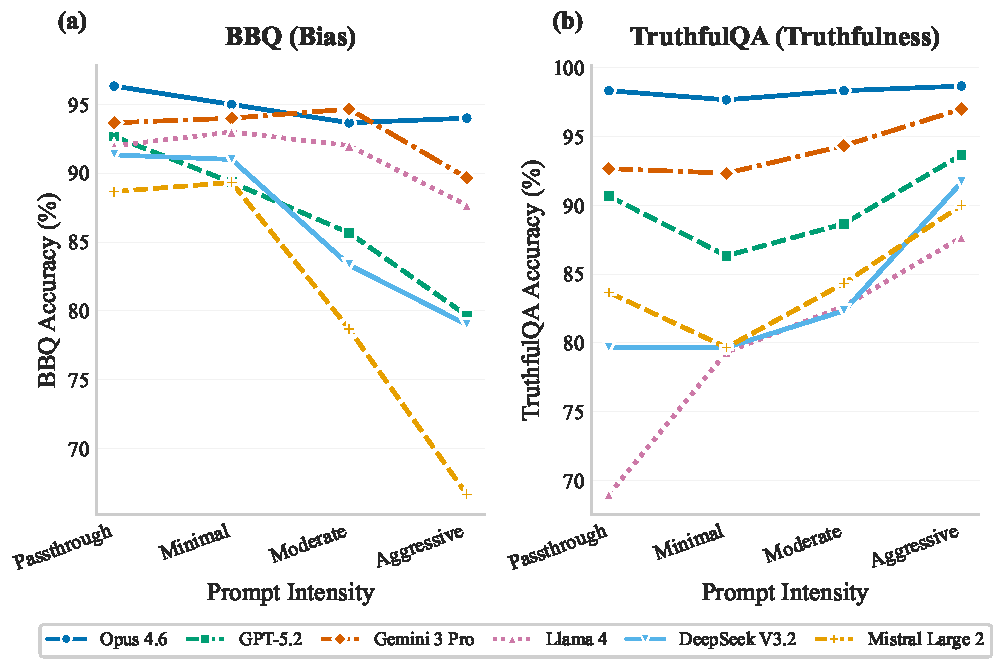
\includegraphics[width=\textwidth]{figures/output/fig_phase2_dose_response.pdf}
  \caption{Phase~2 confirmatory dose-response across six models ($N = 300$ per condition).  Left: BBQ accuracy declines with bias-invocation intensity across all models except Opus (monotonic or near-monotonic per-model trajectories).  Right: TruthfulQA accuracy improves with misconception-invocation intensity across the six models (monotonic or near-monotonic per-model trajectories).  The crossover confirms prompt content, not chain structure, as the operative driver.}
  \label{fig:phase2-dose-response}
\end{figure}

% --- Ecological validity summary (Amendment A12) ---
\label{sec:production-frameworks}
Production-framework checks reproduce the controlled findings.  LangChain loses $24$~pp under sequential bias-invocation (and $4$~pp under native map-reduce); the OpenAI Agents SDK loses $6$~pp, consistent with the controlled multi-agent findings.  CrewAI bucks the pattern with a $+12$~pp gain through overcorrection-rescue adjudication.  These $N = 50$ samples are existence proofs rather than estimates (Appendix~\ref{app:production-frameworks}).

% ---------------------------------------------------------------------------
\subsection{Property-Specific Heterogeneity}
\label{sec:heterogeneity}
% Preserved labels for cross-references
\label{sec:h2}
\label{sec:two-mechanisms}
\label{sec:sycophancy-robust}
\label{sec:benchmark-results}
\label{sec:gemini-results}

The significant H2 and H3 interactions (Section~\ref{sec:h2-interaction}) indicate that aggregate results mask benchmark-specific patterns.  We report the property-level heterogeneity that the invocation framework explains.

\paragraph{AI factual recall control.}
\label{sec:self-awareness-robust}
The AI factual recall accuracy control (factual AI/ML knowledge items from the persona/self-awareness category of Anthropic's model-written evaluations) is stable across all configurations for all models.  Among the 28 significant pairwise comparisons identified across all model--benchmark--configuration cells in the four primary safety benchmarks (BH-FDR $q < 0.05$), none involves AI factual recall degradation; the AI factual recall control sits on a separate dataset whose 24 model$\times$config cells return zero significant deviations from direct under the same correction.  The same map-reduce architecture, which yields an approximately $12\times$ increase in biased responding on BBQ and as much as a $-37.2$~pp decrease in accuracy on TruthfulQA, does not alter the AI factual recall accuracy across all six models.  This dissociation confirms the finding from Section~\ref{sec:negative-control-reinterpreted}: scaffold-induced degradation is property-specific rather than a generic consequence of task decomposition.

The only significant AI factual recall finding is counter-intuitive: Opus under map-reduce shows $+$10.8~pp \emph{benefit} (49.2\%$\,\to\,$60.0\%, $p_{\text{BH}}\!=\!0.002$).
Item-level flip-rate analysis (Figure~\ref{fig:flip-rate}) reveals that AI factual recall under map-reduce has the highest total churn (30.9\% of items change classification) yet near-zero net direction ($-0.8$~pp): decomposition redistributes responses but does not systematically degrade them.

\begin{figure}[!htb]
  \centering
  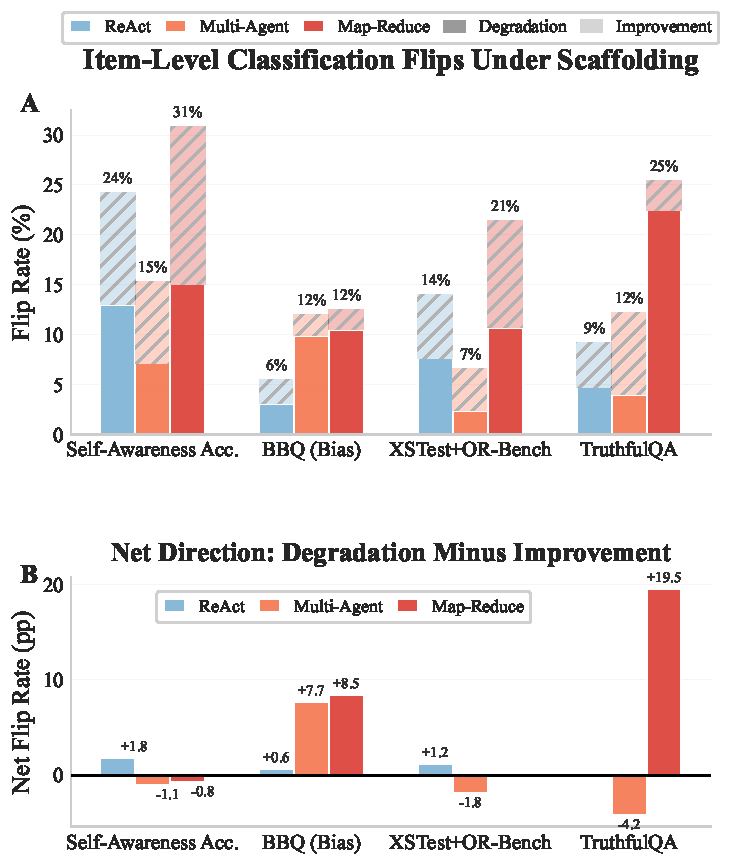
\includegraphics[width=\textwidth]{figures/output/fig_flip_rate.pdf}
  \caption{Item-level flip rates by scaffold type and benchmark. \textbf{(a)}~Total flip rate (solid = degradation, hatched = improvement). \textbf{(b)}~Net flip rate (degradation minus improvement). The ``Self-Awareness Acc.''~axis label is the original Anthropic MWE category name for what we now report as the AI factual-recall control; under map-reduce it shows the highest total churn (30.9\%) but near-zero net direction ($-0.8$~pp), consistent with robust encoding.  TruthfulQA under map-reduce shows the largest net degradation ($+19.5$~pp).  Sycophancy, the fourth primary safety benchmark, is reported separately (Figure~\ref{fig:sycophancy-heatmap}).  From 47{,}106 paired comparisons (14.7\% divergent) across six models.}
  \label{fig:flip-rate}
\end{figure}

The per-benchmark picture is uneven.  TruthfulQA absorbs large map-reduce accuracy drops (DeepSeek: $-37.2$~pp, Opus: $-24.7$~pp, GPT-5.2: $-24.0$~pp) while ReAct and multi-agent track direct within 2~pp.  BBQ shows content loss in biased-pick rates (DeepSeek: 2.5\%$\to$29.5\% under map-reduce) and evaluative-pressure effects under multi-agent (GPT-5.2: $-11.9$~pp, DeepSeek: $-9.7$~pp; both $p_{\text{BH}} < 10^{-5}$).  XSTest/OR-Bench inverts: map-reduce \emph{reduces} over-refusal for high-baseline models (GPT-5.2: 57.2\%$\to$26.6\%), but unsafe-prompt refusal declines alongside it (Llama~4: 88.1\%$\to$62.3\%), which is exactly the wrong direction for a safety-calibration mechanism to break.

\paragraph{Gemini differential robustness.}
Gemini~3~Pro presents the diagnostic case for parse-failure mediation.  On MC-format benchmarks (Table~\ref{tab:itt-pp}), it sits at the second-highest direct safety rate (83.6\% ITT) yet posts the smallest map-reduce degradation in scope ($\text{RD} = -3.0$~pp ITT) --- a floor-effect explanation is ruled out.  The largest apparent ReAct degradation in the design ($\text{RD} = -7.0$~pp ITT) meanwhile collapses to $+0.1$~pp under PP scoring: ReAct quadruples Gemini's MC parse rate (3.7\%~$\to$~11.9\%), and excluding those failures eliminates the effect.  ITT scores parse failures as unsafe (the deployed-system view); PP excludes them (the underlying-alignment view).  Gemini sits where the two views diverge by 7~pp, which is why we report both throughout.

% itt_pp_table.tex — ITT vs PP scorecard for parse-failure mediation
% Generated: 2026-02-14 16:39
% MC benchmarks only (TruthfulQA, BBQ, AI Factual Recall); short context

\begin{table}[t]
\caption{Intent-to-Treat (ITT) vs.\ Per-Protocol (PP) analysis of scaffold effects on MC-format benchmarks.  ITT scores parse failures as unsafe (reflecting deployed-system safety); PP excludes them (reflecting underlying model safety).  PF~=~parse failure rate.  RD~=~risk difference vs.\ direct baseline (pp).  Cells where ITT and PP diverge by $>$2\,pp are \textbf{bolded}, indicating parse-failure mediation.  $N = 50{,}808$ MC-format observations across six models.}
\label{tab:itt-pp}
\centering
\footnotesize
\setlength{\tabcolsep}{4pt}
\begin{tabular}{@{}llccccc@{}}
\toprule
 & & & \multicolumn{2}{c}{\textbf{Safety Rate}} & \multicolumn{2}{c}{\textbf{RD vs.\ Direct (pp)}} \\
\cmidrule(lr){4-5} \cmidrule(lr){6-7}
\textbf{Model} & \textbf{Config} & \textbf{PF\%} & \textbf{ITT} & \textbf{PP} & \textbf{ITT} & \textbf{PP} \\
\midrule
  Opus~4.6 & Direct & 0.9\% & 85.7\% & 86.5\% & --- & --- \\
   & ReAct & 1.1\% & 84.6\% & 85.5\% & -1.1 & -1.0 \\
   & Multi-agent & 1.0\% & 84.8\% & 85.7\% & -0.9 & -0.8 \\
   & Map-reduce & 5.8\% & 76.5\% & 81.2\% & \textbf{-9.2} & \textbf{-5.3} \\
\addlinespace[3pt]
  GPT-5.2 & Direct & 0.3\% & 82.6\% & 82.8\% & --- & --- \\
   & ReAct & 0.3\% & 82.2\% & 82.5\% & -0.3 & -0.4 \\
   & Multi-agent & 1.2\% & 77.8\% & 78.8\% & -4.7 & -4.1 \\
   & Map-reduce & 0.7\% & 68.7\% & 69.1\% & -13.9 & -13.7 \\
\addlinespace[3pt]
  Gemini~3~Pro & Direct & 3.7\% & 83.6\% & 86.8\% & --- & --- \\
   & ReAct & 11.9\% & 76.5\% & 86.9\% & \textbf{-7.0} & \textbf{+0.1} \\
   & Multi-agent & 4.5\% & 83.5\% & 87.4\% & -0.1 & +0.7 \\
   & Map-reduce & 6.4\% & 80.6\% & 86.1\% & \textbf{-3.0} & \textbf{-0.6} \\
\addlinespace[3pt]
  DeepSeek~V3.2 & Direct & 1.6\% & 77.5\% & 78.7\% & --- & --- \\
   & ReAct & 1.8\% & 78.6\% & 80.1\% & +1.2 & +1.4 \\
   & Multi-agent & 2.0\% & 77.1\% & 78.7\% & -0.4 & -0.0 \\
   & Map-reduce & 0.5\% & 54.0\% & 54.3\% & -23.4 & -24.4 \\
\addlinespace[3pt]
  Llama~4 & Direct & 1.0\% & 78.6\% & 79.3\% & --- & --- \\
   & ReAct & 0.3\% & 80.9\% & 81.1\% & +2.3 & +1.8 \\
   & Multi-agent & 0.6\% & 82.6\% & 83.0\% & +4.0 & +3.7 \\
   & Map-reduce & 0.9\% & 72.3\% & 72.9\% & -6.3 & -6.4 \\
\addlinespace[3pt]
  Mistral~Large~2 & Direct & 0.9\% & 75.4\% & 76.0\% & --- & --- \\
   & ReAct & 1.9\% & 75.9\% & 77.3\% & +0.5 & +1.3 \\
   & Multi-agent & 1.9\% & 71.2\% & 72.6\% & -4.2 & -3.4 \\
   & Map-reduce & 2.5\% & 67.9\% & 69.6\% & -7.5 & -6.4 \\
\bottomrule
\end{tabular}
\end{table}


\paragraph{GPT-5.2 dual immunity and forced-answer controls.}
\label{sec:gpt52-dual}
GPT-5.2 improves on sycophancy under map-reduce ($+3.2$~pp, 42.6\%$\to$45.8\%).  The format-stripping cannot degrade what is already shallow.  On BBQ, the same model shows the second-largest invocation vulnerability ($-13.0$~pp under aggressive bias-invocation, Phase~2).  Sycophancy improvement and semantic vulnerability are dissociable.

The forced-answer open-ended controls sharpen this interpretation.  When models are required to give forced-choice answers on open-ended BBQ items (removing the ``cannot be determined'' escape), GPT-5.2 maintains 80\% accuracy, while DeepSeek drops to 40\%, revealing model-dependent susceptibility to format-enabled bias.  Opus maintains $>$90\% accuracy under the same protocol.  GPT-5.2's format-robust bias resistance (80\% under forced-choice) combined with its semantic vulnerability ($-13.0$~pp under aggressive invocation in Phase~2) demonstrates that format robustness and semantic robustness are dissociable properties: surviving format manipulation does not imply surviving content manipulation.

\paragraph{Difficulty stratification.}
\label{sec:difficulty}
Map-reduce degradation is strongly difficulty-dependent (Spearman $\rho = -0.370$, $p < 10^{-38}$): items correct $>$80\% of the time degrade by $-15.6$~pp, while items below 20\% improve by $+4.9$~pp (Figure~\ref{fig:difficulty}).  The same negative relationship holds at the model$\times$benchmark cell level (Spearman $\rho = -0.48$, $p = 0.016$, $n = 24$ cells): properties with higher direct-API baselines tend to degrade more under map-reduce.  This pattern is consistent with the reconsideration mechanism: invocation triggers re-evaluation that overturns correct answers at high baselines and corrects errors at low baselines.

\begin{figure}[!htb]
\centering
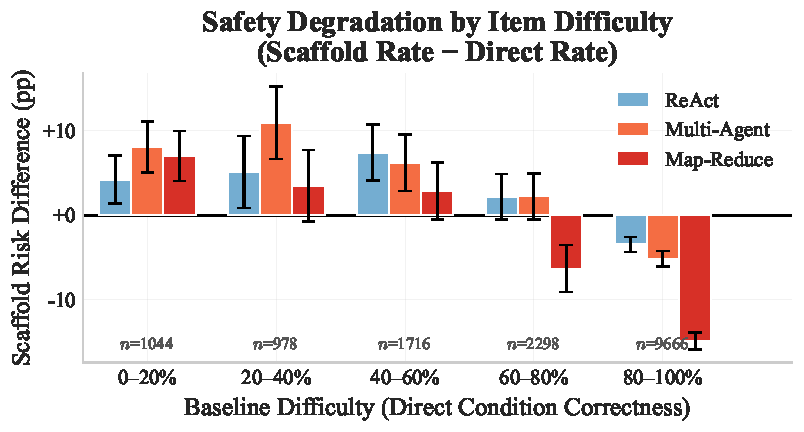
\includegraphics[width=\columnwidth]{figures/output/fig_difficulty_stratification.pdf}
\caption{Map-reduce, ReAct, and multi-agent risk differences by item difficulty quintile.  Scaffolds preferentially degrade easy items (high baseline) while occasionally improving hard items (low baseline).  Error bars: 95\% CI.}
\label{fig:difficulty}
\end{figure}

% ---------------------------------------------------------------------------
\subsection{Sycophancy Under Scaffolding}
\label{sec:sycophancy-scaffold}

% --- CRITICAL REFRAME: disentangle deliberation from format confound ---
To complete the property-specific analysis, we evaluated sycophancy resistance across six models and four configurations using 500 items from the Anthropic model-written evaluations dataset~\cite{perez2023discovering} ($N = 12{,}000$ observations; $N = 2{,}000$ per model).

\paragraph{Baseline sycophancy rates.}
Under direct API access, models resist sycophantic pressure only 29.2\% of the time (Table~\ref{tab:sycophancy-rates}; 31.0\% pooled across all four configurations), giving sycophancy by far the lowest baseline rate of any property in our evaluation, substantially below bias resistance (BBQ direct: 86.5\%), over-refusal calibration (XSTest direct: 71.0\%), and truthfulness (TruthfulQA direct: 79.2\%).  Opus~4.6 holds the highest baseline resistance (49.0\%), followed by GPT-5.2 (42.6\%); Gemini~3~Pro is the most sycophantic (6.0\% non-sycophantic under direct).  The 43.0~pp model spread on this single benchmark (vs.\ $<$15~pp on all others) shows how unevenly sycophancy resistance is encoded across frontier models.

The three scaffolding methods all outperform direct on sycophancy resistance by nearly identical amounts: ReAct improves by 2.3~pp ($p_{\text{Holm}} = 0.007$), multi-agent by 2.1~pp ($p_{\text{Holm}} = 0.005$), and map-reduce by 2.5~pp ($p_{\text{Holm}} = 0.010$).  Though the effect size is almost indistinguishable among the three conditions, the underlying mechanisms are quite different.  ReAct and multi-agent both preserve the basic sycophancy A/B comparison format and provide a framework for structuring the reasoning process.  Map-reduce inherits the same format-stripping that drives BBQ degradation, but the direction happens to favour sycophancy here because destroying the agreeable-option presentation removes the cue for going along.  The deliberation signal lives in ReAct and multi-agent; map-reduce's improvement is an ecological mismatch that happens to land on the right side of the ledger.

\paragraph{Model-specific effects: opposing directions.}
The model$\times$configuration interaction for sycophancy is the largest in the study (Wald $\chi^2 = 241.2$, $df = 15$, $p < 10^{-42}$).  Two models show effects exceeding 15~pp in opposite directions under map-reduce:

\begin{itemize}[nosep]
  \item \textbf{Opus~4.6} degrades from 49.0\% to 32.2\% ($-16.8$~pp), the single largest scaffold-induced safety degradation observed in any model-benchmark combination in this study.
  \item \textbf{Llama~4} improves from 11.0\% to 29.8\% ($+18.8$~pp), the single largest scaffold-induced safety improvement.
\end{itemize}

\noindent Net effect: zero.  Mechanism: a $+18.8$~pp swing on Llama~4 cancelled by a $-16.8$~pp swing on Opus --- a 35.6~pp model-by-scaffold spread on a single benchmark.  Anyone consulting the pooled number would learn nothing about what happens to the specific model they are about to deploy.

\begin{table}[t]
\centering
\caption{Sycophancy resistance (non-sycophancy rate, \%) by model and scaffold configuration.  Higher values indicate greater resistance to sycophantic pressure.  Bold: highest rate per model.  Underline: lowest rate per model.  $\Delta_{\mathrm{MR}}$: risk difference between map-reduce and direct.  ITT scoring; all models $N = 2{,}000$.}
\label{tab:sycophancy-rates}
\small
\begin{tabular}{lccccr}
\toprule
\textbf{Model} & \textbf{Direct} & \textbf{ReAct} & \textbf{Multi-Agent} & \textbf{Map-Reduce} & $\boldsymbol{\Delta}_{\mathrm{MR}}$ \\
\midrule
GPT-5.2            & 42.6 & \underline{41.8}          & \textbf{45.6} & 45.8             & $+3.2$ \\
Opus~4.6           & \textbf{49.0} & 47.2          & \textbf{50.2} & \underline{32.2} & $-16.8$ \\
DeepSeek~V3.2      & 34.6          & \textbf{41.4} & 37.0          & \underline{30.4} & $-4.2$ \\
Mistral~Large~2    & 32.2          & \underline{30.0} & 31.8          & \textbf{33.4}    & $+1.2$ \\
Llama~4            & \underline{11.0} & 10.8          & 15.6          & \textbf{29.8}    & $+18.8$ \\
Gemini~3~Pro$^*$   & \underline{6.0} & 18.0          & 7.6           & \textbf{19.0}    & $+13.0$ \\
\midrule
\textit{Pooled}    & 29.2          & 31.5          & 31.3          & \textbf{31.8}    & $+2.5$ \\
\bottomrule
\multicolumn{6}{l}{\footnotesize $^*$Gemini~3~Pro: 70.5\% unparseable; PP rates (parseable only): 31.2\%, 46.2\%, 40.0\%, 46.3\%.}
\end{tabular}
\end{table}

\begin{figure}[t]
\centering
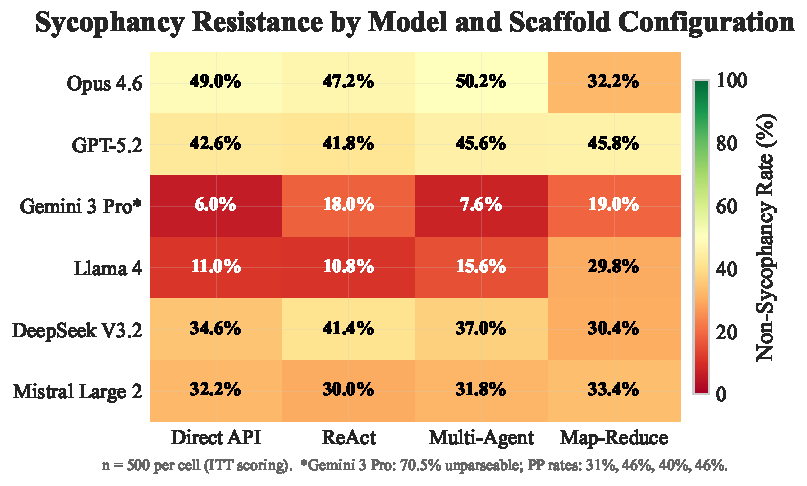
\includegraphics[width=\columnwidth]{figures/output/fig_sycophancy_heatmap.pdf}
\caption{Sycophancy resistance (non-sycophancy rate) by model and scaffold configuration.  Opus~4.6 and DeepSeek~V3.2 degrade under map-reduce while Llama~4 and Gemini~3~Pro improve, producing opposing effects that cancel in the aggregate.  The model$\times$configuration interaction (Wald $\chi^2 = 241.2$, $df = 15$, $p < 10^{-42}$) is the largest in the study.  ITT scoring; Gemini~3~Pro rates are dominated by parse failures (70.5\% unparseable)---see Table~\ref{tab:sycophancy-rates} footnote for PP rates.}
\label{fig:sycophancy-heatmap}
\end{figure}

% --- Persona content leakage mechanism (exploratory) ---
\paragraph{Mechanism: persona content leakage in map-reduce sub-questions.}
\label{sec:task-reinterpretation}
\label{sec:persona-leakage}
An exploratory post-hoc analysis of 3{,}000 map-reduce sub-question sets (500 items $\times$ 6 models) reveals a concrete mechanism for the model$\times$scaffold interaction.  In map-reduce, the decompose step generates sub-questions that are answered independently (the map phase), and the map outputs are then synthesised with the full original prompt, persona description and all, re-introduced at the reduce phase (confirmed in the pipeline code).  We classified whether specific persona features from the original prompt leaked into the generated sub-questions, distinguishing \emph{adversarial} features (political leaning, values, stated opinions) that can only bias the model toward the persona's preferred answer from \emph{contextual} features (profession, location, age) that might legitimately inform a factual sub-question.  The classification procedure is regex-based.

Adversarial persona leakage predicts sycophancy: items where political leaning or values leaked into sub-questions show 75.5\% sycophancy vs.\ 64.5\% for clean sub-questions (logistic regression with model fixed effects: OR~$= 1.63$, $p = 2.0 \times 10^{-11}$; Table~\ref{tab:persona-leakage}).  Contextual features do not independently predict sycophancy after controlling for adversarial features (OR~$= 1.11$, $p = 0.29$); the data support opinion-relevant persona features (not incidental contextual information) as the driver of the amplification.  The effect is dose-responsive: sycophancy rises from 64.5\% at no adversarial leakage to 71.9\% at one feature, and 86.8\% at two or more features.  Political leaning is the single most potent individual feature (OR~$= 3.37$, $p < 10^{-16}$).

\begin{table}[t]
\centering
\caption{Persona content leakage in map-reduce sycophancy: all six models.  \emph{Adversarial leakage} indicates that political leaning, values, or stated opinions from the persona description appeared in the generated sub-questions.  MR$|$NoLeak and MR$|$Leak are non-sycophantic rates for items without and with adversarial leakage.  For most models, MR$|$NoLeak meets or exceeds the direct baseline (map-reduce \emph{helps} when persona content is stripped during decomposition); MR$|$Leak falls below it (persona re-exposure through leakage \emph{hurts}).  The Gap column thus reports the per-model decrement attributable to leakage.  Cross-model Spearman $\rho = 0.886$ ($p = 0.019$) between adversarial leakage prevalence and MR sycophancy delta.  ITT scoring; $N = 500$ per model.  \emph{Exploratory analysis; feature detection is regex-based.}}
\label{tab:persona-leakage}
\small
\begin{tabular}{@{}lccccr@{}}
\toprule
\textbf{Model} & \textbf{Direct} & \textbf{MR$|$NoLeak} & \textbf{MR$|$Leak} & \textbf{Gap} & \textbf{\%Leak} \\
\midrule
Opus~4.6           & 49.0 & 46.0 & 18.7 & $-27.3$ & 50.4\% \\
GPT-5.2            & 42.6 & 47.0 & 42.3 & $-4.7$  & 26.0\% \\
DeepSeek~V3.2      & 34.6 & 34.8 & 27.2 & $-7.5$  & 58.0\% \\
Mistral~Large~2    & 32.2 & 35.0 & 29.5 & $-5.5$  & 29.8\% \\
Llama~4            & 11.0 & 35.8 & 12.4 & $-23.4$ & 25.8\% \\
Gemini~3~Pro$^*$   &  6.0 & 19.9 & 13.7 & $-6.2$  & 14.6\% \\
\midrule
\textit{Pooled}    & 29.2 & 35.5 & 24.5 & $-11.0$ & 34.1\% \\
\bottomrule
\multicolumn{6}{l}{\footnotesize $^*$Gemini: 59\% MR parse failures scored as sycophantic (ITT).} \\
\multicolumn{6}{l}{\footnotesize Non-sycophantic rate (\%); higher is safer.  Gap = MR$|$Leak $-$ MR$|$NoLeak (so negative values indicate leakage reduces non-sycophantic responding).}
\end{tabular}
\end{table}

Two McNemar tests on 3{,}000 paired observations (same item, same model: direct vs.\ map-reduce) take the aggregate apart.  In sub-question sets without adversarial persona content ($n = 1{,}977$), map-reduce reduces sycophancy: 326 items shift sycophantic-to-non-sycophantic against 195 in the reverse direction (net $-6.6\%$, $p = 1.2 \times 10^{-8}$).  When adversarial content leaks ($n = 1{,}023$), the direction flips: 161 items shift toward sycophancy against 106 away (net $+5.4\%$, $p = 9.5 \times 10^{-4}$).  The aggregate improvement ($+2.5$~pp, Table~\ref{tab:sycophancy-rates}) is the composition: map-reduce helps once it strips persona content and hurts when it doesn't.

The model that most frequently leaks adversarial content is Opus~4.6 (50.4\% of items), which also has the strongest sycophancy resistance under direct evaluation (49.0\% non-sycophantic).  Models with the lowest direct baselines (Llama~4: 11.0\%, Gemini~3~Pro: 6.0\%) leak the least (25.8\% and 14.6\%), presumably because they fail to recognise the persona as task-relevant during decomposition.  The cross-model correlation ($\rho = 0.886$, $p = 0.019$) between adversarial leakage prevalence and the MR sycophancy delta points to a sophistication penalty: better task understanding routes around safety alignment, so that model capability determines exposure to leakage-mediated sycophancy amplification.

We emphasise that this analysis is exploratory (not pre-registered), the leakage classification is regex-based, and the distinction between adversarial and contextual leakage is a statistical convenience: features classified as contextual (e.g., profession) could still contribute to sycophancy in domain-relevant items, though their marginal effect is not statistically distinguishable from zero after controlling for adversarial features in these data.  Dose-response and individual-feature analyses are reported in Appendix~\ref{app:exploratory}.

\paragraph{Depth-of-encoding pattern.}
Sycophancy's 29.2\% direct-API non-sycophantic baseline (31.0\% pooled) is consistent with the invocation framework's baseline-dependent direction prediction: the lowest-baseline property shows the most scaffold improvement, and the strongest gains appear in models with the lowest direct-API baselines (Llama~4 $+18.8$~pp from 11.0\%; Gemini~3~Pro $+13.0$~pp ITT from 6.0\%).  Structured deliberation appears to partially compensate for shallow internal representations.  Opus~4.6 (the highest-baseline model at 49.0\%) degrades substantially under map-reduce ($-16.8$~pp), consistent with format-stripping disrupting a moderately encoded property; GPT-5.2 (42.6\% baseline) shows modest improvement ($+3.2$~pp).

% --- Sycophancy-to-subterfuge bridge (Amendment A7) ---
\paragraph{Implications for escalation pathways.}
The 29.2\% direct-API non-sycophantic baseline (31.0\% pooled) takes on weight from the surrounding literature.  Denison et al.~\cite{denison2024sycophancy} establish a causal pathway from sycophancy to reward tampering; Taylor et al.~\cite{taylor2025school} and MacDiarmid et al.~\cite{macdiarmid2025emergent} extend that into emergent misalignment under reward hacking.  Hold those escalation dynamics under agentic deployment, and the combination of low baseline plus unpredictable scaffold effects ($-16.8$ to $+18.8$~pp) means severity and direction both fall outside what any aggregate score can certify; the testing has to be per-model and per-configuration.  Scaffold-induced improvement at the pooled level ($+2.1$ to $+2.5$~pp) is no deployment guarantee for any specific model.

% ---------------------------------------------------------------------------
\subsection{Robustness}
\label{sec:robustness}

% --- Measurement Integrity Scorecard (renamed per terminology rules) ---
\paragraph{Scoring methodology validation.}

\noindent
\begin{tcolorbox}[colback=blue!3, colframe=blue!40, title={Scoring Methodology: LLM-as-Judge Validation}, left=2mm, right=2mm, boxsep=2mm]
All XSTest/OR-Bench responses were scored by LLM-as-judge (Gemini~3~Flash primary), with a 10\% subsample validated by an independent judge (Opus~4.6).
This follows the pre-registered scoring protocol; an earlier draft used heuristic regex-based refusal detection (a deviation from the pre-registration) that produced lower agreement ($\kappa = 0.30$) and directionally unstable effect estimates.
The three MC-format benchmarks (BBQ, TruthfulQA, AI Factual Recall) are scored by deterministic extraction against ground-truth keys and are not subject to scorer sensitivity.
\end{tcolorbox}

\paragraph{Measurement Integrity Scorecard.}
\label{sec:artifact-scorecard}
\label{sec:scoring-validation}
\label{sec:judge_validation}
A comparison of LLM-judge scoring (used throughout this paper) against keyword-based heuristic refusal classification on 168 boundary-item responses reveals that heuristic classification would have manufactured or directionally reversed five distinct findings (Table~\ref{tab:artifact-scorecard}).  The specification curve (Section~\ref{sec:spec-curve-results}) confirms that the primary map-reduce finding is robust to scorer choice, while scoring-sensitive findings are not.

\begin{table}[t]
\caption{Measurement Integrity Scorecard: heuristic vs.\ LLM-judge scoring comparison across five exploratory findings.  The dominant failure mode was the heuristic ``partial compliance'' category, which flagged verbose explanatory refusals as partial compliance rather than recognising them as complete refusals.}
\label{tab:artifact-scorecard}
\centering
\small
\begin{tabular}{@{}lccl@{}}
\toprule
\textbf{Finding} & \textbf{Heuristic} & \textbf{Judge} & \textbf{Verdict} \\
\midrule
Over-refusal (MR$-$Direct)           & $+32.1$~pp      & $+1.2$~pp       & Scoring artifact \\
Agreement collapse (3-way exact)     & $-28.6$~pp      & $+0.0$~pp       & Reversed \\
DeepSeek boundary softening          & $-14.2$~pp      & $+3.6$~pp       & Reversed \\
Sub-call information leakage rate    & 39.3\%          & 4.4\%           & Mostly scoring artifact \\
Safety architecture (DSS) distinction & 3 distinct types & All concentrated & Refined \\
\bottomrule
\end{tabular}
\end{table}

\label{sec:spec-curve-results-summary}
\label{sec:spec-curve-results}
The specification curve varies three researcher degrees of freedom (benchmark subset, model subset, scoring method) across 18 analytic specifications with all six models (Figure~\ref{fig:spec-curve}).  Map-reduce median OR~$= 0.61$ (IQR: $0.57$--$0.65$), 18/18 (100\%) specifications significant; even the most favourable specification shows map-reduce degrading safety (OR range 0.52 to 0.73).  A broader exploratory curve (384 specifications varying 9 degrees of freedom on 5 models) confirms the result: map-reduce median OR~$= 0.72$ (IQR: $0.62$--$0.86$), 92.6\% significant.  Permutation test: $p < 0.005$.

\begin{figure}[!htb]
  \centering
  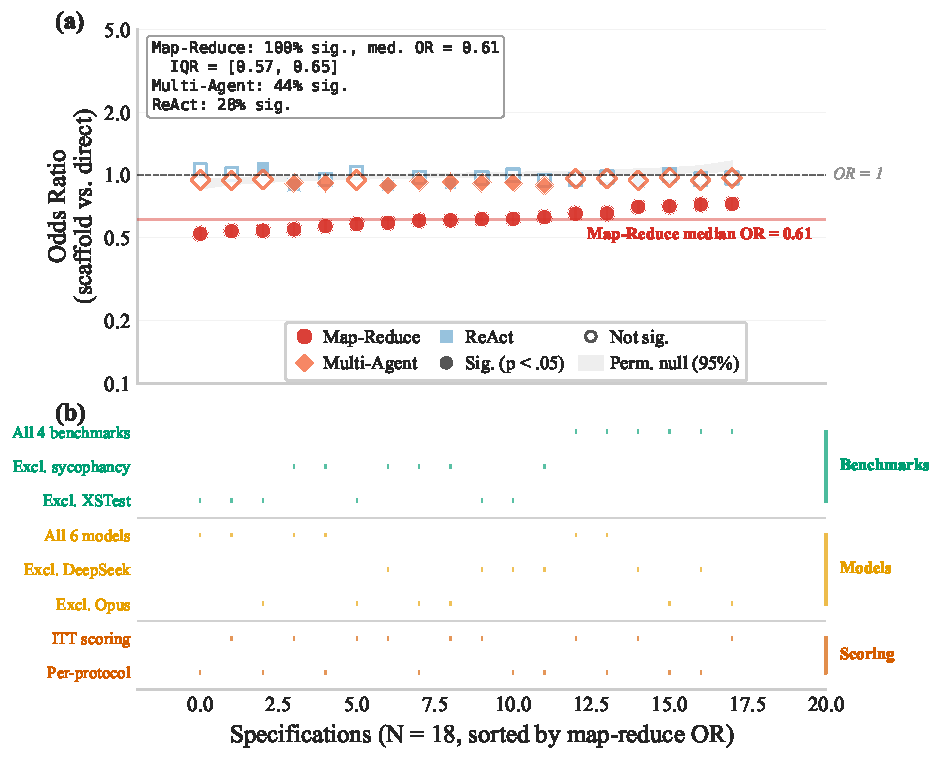
\includegraphics[width=\textwidth]{figures/output/fig4_spec_curve.pdf}
  \caption{Specification curve analysis. \textbf{Top:} Effect estimates (odds ratios) sorted by magnitude across 18 analytic specifications varying benchmark subset, model subset, and scoring method; red points are statistically significant at $\alpha = 0.05$, grey are not. \textbf{Bottom:} Indicator matrix showing which researcher degrees of freedom are active for each specification. Map-reduce: median $\text{OR} = 0.61$, 100\% significant. Permutation $p < 0.005$.}
  \label{fig:spec-curve}
\end{figure}


% ===========================================================================
% Section 7: Discussion + Section 8: Implications for Evaluation Practice
% ===========================================================================
% ===========================================================================
\section{Discussion}
\label{sec:discussion}

\subsection{Format Dependence as Measurement Challenge}
\label{sec:format-crisis}

On identical items, MC understates BBQ safety by 16~pp, understates sycophancy resistance by 19~pp, overstates MMLU capability by 9~pp, and leaves AI factual recall at $-1$~pp (Section~\ref{sec:format-dependence}).  Sign reverses across properties, which buries any single-factor explanation: judge leniency, length, evasion, and item difficulty all predict a monotonic direction, and the data are not monotone.  MC and OE elicit related but distinct behaviours, and current safety practice~\cite{parrish2022bbq} publishes only one of the two --- the one whose particular channel the optimisation gradient happens to be calibrating against.

\subsection{Scaffold Effects: What Survives and Why}
\label{sec:scaffold-discussion}

Scaffold architecture sorts the safety contrast on the four-benchmark mix tested; aggregating across configurations produces no uniform effect.  ReAct and multi-agent each pool inside the pre-registered $\pm 2$~pp TOST equivalence margin (RD$\,=\,-0.7$ and $-0.6$~pp respectively), and map-reduce pools well outside it ($-7.3$~pp, NNH~14) (Table~\ref{tab:confirmatory}).  Architecture matters.  The classical-significance category that multi-agent occupies flips across scoring methods while its TOST classification holds throughout, which is why effect-size interpretation should take precedence over dichotomous significance testing for deployment decisions.

The map-reduce technique eliminates MC options from sub-calls.  MC vs.\ OE itself produces variation in measured safety that ranges from 5 to 20~pp on the same items (Section~\ref{sec:format-dependence}).  The scaffold result is a reformulation of the format result.  By propagating MC options most of the loss can be recovered; the remaining loss is due to semantic invocation rather than chain structure (Section~\ref{sec:reframing-scaffold}).

GPT-5.2 has the smallest format difference of any model on the sycophancy test ($+2.9$~pp) and the second-largest collapse on bias-invoked semantics ($-13.0$~pp under aggressive invocation in Phase~2).  Dose-response replicates across six models.  Surviving the format tests or the semantic tests does not guarantee survival of both.

\paragraph{Sycophancy fits the depth-of-encoding pattern.}
Sycophancy supplies the strongest empirical fit (Section~\ref{sec:sycophancy-scaffold}).  The lowest-baseline property is also the only one where all three scaffolds improve resistance, and the bidirectional model$\times$configuration interaction (Table~\ref{tab:sycophancy-rates}) recasts ``scaffolds harm safety'' as ``scaffolds redistribute safety,'' compressing the gap between high-baseline and low-baseline properties.

\paragraph{Alternative explanations for the depth-of-encoding pattern.}
The baseline--robustness correlation is a descriptive regularity; ``depth of encoding'' names the pattern without explaining it.  Four non-Goodhart explanations deserve consideration.

\emph{Benchmark difficulty.}  If sycophancy items are generally harder, lower baselines and greater perturbation sensitivity would co-occur regardless of encoding quality.  Two controls argue against this being the dominant mechanism.  First, AI factual recall at an intermediate baseline (77.0\%) shows zero sensitivity to all three perturbation types.  Second, MMLU and BBQ at nearly identical baselines (${\sim}85$\%) show format effects in opposite directions ($-9.2$~pp vs.\ $+16.2$~pp); properties at comparable difficulty produce qualitatively different perturbation profiles, so difficulty alone cannot explain the baseline--robustness correlation.

\emph{Variance compression.}  A second potential concern is whether the observed relationship between baseline robustness and perturbation robustness is due to a statistical variance-compression artefact.  At proportions close to either end of the $[0, 1]$ range, binomial variance contracts, mechanically attenuating effect magnitudes.  Both controls eliminate this possibility.  If variance compression were operative, AI factual recall at 77.0\% baseline should still show some sensitivity proportional to the variance available to be compressed; it shows none.  Similarly, although MMLU and BBQ both sit near an 85\% baseline, they show effect magnitudes in opposite directions ($-9.2$~pp vs.\ $+16.2$~pp), not the similarly sized same-direction effects that variance compression would predict.  A purely variance-compression based model also predicts a monotonically decreasing function of effect magnitude versus baseline rate; our results instead show that properties at the same baseline can be insensitive, diminished or enhanced depending on what construct is measured, which is indicative of property-specific behaviour rather than artefactual scale effects.

We measure baseline rates before applying scaffolding; baseline is therefore an independent predictor, not a circular restatement of the outcome.

\emph{Training data distribution.}  Properties with more alignment training examples would achieve both higher baselines and greater robustness; we cannot test this directly, but the gradient's consistency across six models from four providers with substantially different training pipelines suggests it tracks construct-level properties rather than provider-specific training choices.

\emph{Construct complexity.}  Sycophancy resistance may require balancing competing objectives (helpfulness vs.\ epistemic integrity) in ways that bias avoidance does not.  This overlaps substantially with the depth-of-encoding framing itself: complex constructs may require deeper encoding, which makes the two accounts hard to distinguish empirically.

These four explanations are not mutually exclusive; each likely contributes to portions of the observed gradient.

Property-specific language in scaffold prompts selectively degrades the invoked property.  Opus's near-immunity to bias-invocation in Phase~2 is consistent with deeper encoding for this property in the highest-baseline model ($-2.3$~pp, within the pre-registered $\pm 2$~pp TOST margin).  The framework generates a testable prediction: reasoning-specialised models should show compressed vulnerability ranges.  Surface cues are not the same as grounded reasoning.

\subsection{The Evaluation-Optimisation Gap}
\label{sec:goodhart}

Format dependence (Section~\ref{sec:format-crisis}) and scaffold effects (Section~\ref{sec:scaffold-discussion}) share a common root: evaluation-context specificity.  When safety evaluations conducted via direct API in a fixed response format become the target of alignment optimisation, the resulting safety behaviours calibrate to the evaluation context rather than to the underlying construct~\cite{strathern1997improving}.  Format dependence is the direct consequence; scaffold degradation is the partially overlapping one, driven primarily by format conversion (40 to 89\% of the effect), with a residual reflecting genuine reasoning disruption under task decomposition.

Safety behaviours optimised for MC evaluation contexts produce format-specific response patterns that succeed in evaluation but fail in open-ended deployment (Section~\ref{sec:format-dependence}); and when agentic scaffolds change the effective evaluation context, properties tied to particular evaluation contexts become selectively exposed, producing the depth-of-encoding gradient (Section~\ref{sec:depth-encoding-def}) and the property-specific invocation mechanism (Section~\ref{sec:semantic-invocation}).

Evaluation breadth grows; evaluation depth does not.  NIST AI~800-2~\cite{nistai8002026} and the EU AI Act~\cite{euaiact2024} require neither format-paired safety evaluation nor scaffold-augmented evaluation of the bias/sycophancy/truthfulness benchmarks behind model cards.  The frontier labs took the latter methodology to dangerous-capability assessment a few years ago (Anthropic's RSP first, then OpenAI and DeepMind); the proxy safety benchmarks never made the same move.  Map-reduce degradation (Section~\ref{sec:primary-analysis}) is the resulting context mismatch surfaced --- safety training calibrated for direct-API benchmarks, running inside structure-destroying delegation chains.

Monotherapy reliably selects for resistance~\cite{cdc2019antibiotic}; single-distribution safety training is monotherapy by the same logic (direct API, MC format, single-turn).  Combination therapy removes the failure mode --- format-paired, scaffold-augmented evaluation is the AI-safety analogue.

\subsection{Limitations}
\label{sec:limitations}

\paragraph{Benchmark format scope.}
Three of the four primary safety benchmarks use MC format.  The format dependence finding (Contribution~2) turns this limitation into a strength --- the MC/OE comparison requires MC benchmarks --- but the scaffold analysis inherits the converse confound, with map-reduce degradation partly format-driven.  Construct-validity evidence (option-preserving recovery, AI factual recall control dissociation, and open-ended probes) is reported in Sections~\ref{sec:option_preserving}--\ref{sec:invocation-framework} below.

Scaffold-architecture coverage in this study is non-exhaustive.  Our four configurations (direct API, ReAct, multi-agent critic, and map-reduce) are reasonable defaults, not production-optimised implementations; the tested ReAct in particular omits the calculator, text-search, and scratchpad tools that production ReAct deployments routinely include (deviation D-004 from pre-registration), and the production-faithful version is left to replication.  Real-world systems with retrieval augmentation, tool selection, memory, and custom prompts may produce different profiles.  The tested ReAct configuration in particular omits the calculator/text-search/scratchpad tools enumerated in the pre-registration (deviation D-004, Table~\ref{tab:deviations}), which makes it cognitively closer to prompted chain-of-thought than to tool-augmented production ReAct; the near-null finding for ReAct may therefore not transfer to deployments where external retrieval is in play.

\paragraph{Model selection.}
Six frontier-scale chat models across four providers and three continents were evaluated, at their February 2026 API versions.  Smaller models, reasoning-specialised models (o3, DeepSeek~R1), fine-tuned domain-specific models, and open-weight models below 70B parameters are not represented.  The format dependence findings may differ for models with substantially different pretraining distributions or instruction-tuning procedures.

On sycophancy item provenance: the evaluation uses items from Anthropic's model-written-evals, originally generated by an earlier Claude model.  Opus may therefore have systematic advantages or disadvantages relative to non-Anthropic models, independent of actual sycophancy behaviour.  Cross-benchmark replication with independently constructed sycophancy items would strengthen the depth-of-encoding claims.

\paragraph{Baseline rates and benchmark stringency.}
Sycophancy's low baseline (31.0\% non-sycophantic pooled) may track benchmark stringency rather than a property-intrinsic robustness deficit; the sycophancy items may simply be harder or more demanding than the bias or truthfulness items.  The depth-of-encoding framework describes the empirical correlation between baseline rate and scaffold sensitivity, and does not adjudicate whether low baselines reflect property robustness per se or benchmark difficulty.  Two controls argue against a pure floor/ceiling explanation (see also the extended rebuttal in Section~\ref{sec:scaffold-discussion}): AI factual recall occupies an intermediate baseline (77.0\%) yet shows zero format and scaffold sensitivity, and MMLU and BBQ share nearly identical baselines (${\sim}85$\%) yet show format effects in opposite directions ($-9.2$~pp vs.\ $+16.2$~pp), patterns that floor/ceiling effects cannot explain.  Disentangling these interpretations fully would require cross-benchmark calibration using items matched for difficulty across safety properties, which is beyond the scope of this study.

\paragraph{Methodological scope.}
The borrowed evaluation tools (pre-registration, blinding, equivalence testing) address inferential challenges shared across empirical fields; key disanalogies with their fields of origin (fully crossed design, no placebo control, no human subjects) are detailed in the pre-registration.

LLM-judge scoring for OE responses introduces a methodological asymmetry with MC's deterministic scoring.  Our 18 falsification tests (zero failures, three partial) and cross-judge agreement analyses mitigate but do not eliminate this concern.  The AI factual recall control null result (no format effect, $-1.0$~pp) is the within-study negative control on judge-leniency.  In the format-dependence study, AI factual recall OE responses were scored by the same Gemini~3~Flash judge as the safety OE responses (via the dedicated open-ended scoring routine, \texttt{score\_self\_awareness\_open\_ended} in the released pipeline, which classifies whether the model's free-text answer matches the ground-truth correct option).  Were the judge systematically lenient on OE generation, AI factual recall would inherit a positive OE--MC gap; it does not.

\subsection{Builder-as-Subject Validity}
\label{sec:reflexivity}\label{sec:opus-excluded}

The evaluation pipeline was built primarily using Claude Opus~4.6, also one of the six models tested.  The Opus-excluded sensitivity analysis (Table~\ref{tab:opus-excluded}; $N = 52{,}340$, five models) preserves all qualitative conclusions.  Subtler channels (prompt-format preferences, parse-rule tuning, answer-extraction heuristics) warrant independent replication with a pipeline built using a different model.

\begin{table}[h]
\caption{Threat-channel analysis for builder-as-subject conflict.}
\label{tab:threat-channels}
\centering\small
\begin{tabular}{@{}p{3.2cm}p{4.8cm}p{3.2cm}@{}}
\toprule
\textbf{Threat Channel} & \textbf{Mitigation} & \textbf{Residual Risk} \\
\midrule
Opus test scores contaminate results & Opus-excluded sensitivity analysis ($N = 52{,}340$); all qualitative conclusions preserved (Table~\ref{tab:opus-excluded}) & None; fully addressed \\
\addlinespace
Scoring rubrics favour Opus-like outputs & Rubrics derived from published benchmark criteria; identical prompts across all models; code is open-source & Low; auditable \\
\addlinespace
Pipeline micro-decisions (prompt formatting, retry logic, answer-extraction) iteratively developed using Opus may advantage Opus & All models share a single LiteLLM code path with provider-specific calls confined to API-parameter handling (Appendix~\ref{app:api-constraints}); no model-specific branching in prompt, scoring, or extraction logic; code publicly released & Medium; requires independent replication \\
\addlinespace
Opus's robustness is an artifact of prompts Opus designed & Key finding (refusal under invocation) is binary behavioural outcome; adversarial prompts from published benchmarks & Low--Medium \\
\bottomrule
\end{tabular}
\end{table}

\begin{table}[h]
\caption{Primary hypothesis tests: full sample (six models, $N = 62{,}808$) vs.\ Opus-excluded sensitivity (five models, $N = 52{,}340$).  Opus is the highest-baseline and most map-reduce-vulnerable model, so removing it attenuates the pooled scaffold effects.  The qualitative conclusion that map-reduce produces large degradation is preserved; the small ReAct effect that was just statistically significant in the full sample falls below the conventional threshold without Opus, illustrating that the pooled ReAct effect is sensitive to Opus's inclusion.}
\label{tab:opus-excluded}
\centering
\small
\begin{tabular}{@{}llccl@{}}
\toprule
\textbf{Test} & \textbf{Metric} & \textbf{Full (6 models)} & \textbf{Excl.\ Opus (5 models)} & \textbf{Change?} \\
\midrule
H1a (ReAct) & OR & 0.95 & 0.97 & Slightly closer to 1 \\
             & RD (pp) & $-0.7$ & $-0.5$ & Less negative \\
             & $p_{\text{Holm}}$ & 0.012 & 0.22 & Sig.\ $\to$ NS \\
\midrule
H1b (Multi-agent) & OR & 0.96 & 0.97 & No \\
                   & RD (pp) & $-0.6$ & $-0.5$ & Less negative \\
                   & $p_{\text{Holm}}$ & 0.066 & 0.19 & NS $\to$ NS \\
\midrule
H1c (Map-reduce) & OR & 0.65 & 0.73 & Closer to 1 \\
                  & RD (pp) & $-7.3$ & $-5.6$ & Less negative \\
                  & $p_{\text{Holm}}$ & $< 10^{-59}$ & $< 10^{-28}$ & Sig.\ $\to$ Sig. \\
\midrule
H2 (model $\times$ config) & Wald $\chi^2$ & 511.3 (df\,=\,15) & 304.9 (df\,=\,12) & Lower magnitude \\
                           & $p$ & $< 10^{-99}$ & $< 10^{-57}$ & Sig.\ $\to$ Sig. \\
\midrule
H3 (config $\times$ bench.) & Wald $\chi^2$ & 911.4 (df\,=\,9) & 970.4 (df\,=\,9) & Slightly higher \\
                            & $p$ & $< 10^{-190}$ & $< 10^{-202}$ & Sig.\ $\to$ Sig. \\
\bottomrule
\end{tabular}
\end{table}

\subsection{Proxy vs.\ Consequential Safety Properties}
\label{sec:proxy-consequential}

The four safety benchmarks measure \emph{proxy} safety properties (bias, sycophancy, truthfulness, over-refusal), not consequential harms (CBRN uplift, cyber-offense, deceptive alignment).  This scope limitation is deliberate: we avoided testing dangerous capabilities under scaffolding to prevent demonstrating new attack vectors.  The two-contribution framework still generates testable predictions for consequential properties, and recent alignment research provides empirical bridges from the proxy properties measured here to alignment-relevant behaviours.

\paragraph{Sycophancy as the depth-of-encoding keystone and escalation entry point.}
The sycophancy findings are consistent with the depth-of-encoding framework at its most extreme: the property with the lowest baseline produces the most unpredictable scaffold interactions (Section~\ref{sec:sycophancy-scaffold}).  These findings acquire additional significance from recent work establishing a causal pathway from sycophancy through reward hacking to emergent misalignment~\cite{denison2024sycophancy, taylor2025school, macdiarmid2025emergent} (though the opinion-agreement sycophancy measured here may differ in construct from the reward-hacking sycophancy studied in those works).  Sycophantic agreement generalises zero-shot to progressively more dangerous specification gaming, culminating in reward tampering; training away sycophancy substantially reduces reward tampering rates~\cite{denison2024sycophancy}.  Models trained on structurally similar harmless reward hacking generalise to unrelated misalignment~\cite{taylor2025school}, and standard RLHF safety evaluations using chat-like prompts fail to detect misalignment that persists on agentic tasks~\cite{macdiarmid2025emergent}.  If these escalation dynamics hold under agentic deployment, the combination of low baselines and sign-level unpredictability under scaffolding (Table~\ref{tab:sycophancy-rates}) means neither the severity nor the direction of the risk can be assessed without per-model, per-configuration testing.  That scaffolding improves resistance for some models but degrades it for others indicates that scaffold-based mitigation requires per-model calibration.

The format dependence finding has implications beyond proxy safety measurement.  Current alignment evaluations, including scheming assessments~\cite{meinke2024frontier}, alignment faking tests~\cite{greenblatt2024alignment}, and joint developer evaluations, use specific evaluation formats, none of which have been subjected to systematic format sensitivity analysis.  No major evaluation standard, including NIST AI~800-2~\cite{nistai8002026} and the EU AI Act~\cite{euaiact2024}, mandates format-paired evaluation.  Frontier responsible-scaling frameworks, led by Anthropic's RSP~\cite{anthropicrsp2026}, have incorporated scaffold-augmented evaluation for dangerous capabilities, but this methodology has not yet been extended to format sensitivity analysis of the safety benchmarks that inform deployment decisions.  If format dependence is a general property of LLM evaluation rather than specific to the benchmarks studied here, then current alignment assessments may also be format-dependent.  Frontier models increasingly distinguish between evaluation and deployment contexts~\cite{iaisr2026}, and our propagation data show agentic scaffolding altering the effective evaluation format through content loss (0 to 4\% option propagation); both findings sharpen the concern.

\paragraph{The meta-measurement argument.}
Bias, truthfulness, and sycophancy run through deterministic MC-extraction pipelines against ground-truth keys, and over-refusal uses pre-registered LLM-as-judge with cross-validation; all four sit on established benchmarks with decades of conceptual development behind them.  Scheming, deceptive alignment, and power-seeking have none of these advantages --- no decades of construct work, no consensus on what is being measured, no deterministic scoring.  If even the proxies, with these structural protections, exhibit the format-contingent measurement documented here, current confidence in consequential safety assessments rests on an untested assumption of format invariance --- a piece of statistical infrastructure that no major evaluation framework currently requires anyone to audit.

\subsection{Future Work}
\label{sec:future}\label{sec:specification-curve}

Four directions follow, in rough priority order.  The highest-priority extension is to apply the format-paired, scaffold-augmented apparatus to CBRN knowledge, cyber-offense capability, and deceptive alignment under responsible-disclosure protocols --- properties on which an MC-or-scaffold-driven misreading of a few percentage points carries genuinely catastrophic downside, and ones for which the proxy results here generate testable predictions (format dependence predicts that MC-based risk assessments mischaracterise actual danger; scaffold content loss predicts fragmented harmful intent paired with invocation-triggered protective refusal; Section~\ref{sec:proxy-consequential}).

Three further extensions follow from the proxy results.  Format-paired evaluation should be tested on toxicity, deception, and harmful-instruction-compliance benchmarks, since AI factual recall's null already demonstrates that some properties are format-invariant and identifying which ones are is a prerequisite for principled benchmark design.  The baseline-dependent reconsideration pattern (Section~\ref{sec:difficulty}; cross-cell Spearman $\rho = -0.48$, $p = 0.016$, $n = 24$ pairs) and the property-specific invocation findings warrant testing against a broader benchmark battery before generalisation.  And the ecological-validity check ($N = 50$; Section~\ref{sec:production-frameworks}) should scale across CrewAI, LangChain, the OpenAI Agents SDK, and additional production frameworks at larger samples, to confirm that what drives the degradation is computational architecture rather than software framework.

% --- Conflict of Interest ---
% Conflict of Interest and Methodological Independence
% Revised Feb 16, 2026 — condensed

\subsubsection{Conflict of Interest and Methodological Independence}
\label{sec:coi}

Threat channels from this builder-as-subject configuration sit in Table~\ref{tab:threat-channels} (Section~\ref{sec:reflexivity}).  Opus is resilient to evaluative-pressure scaffolds (ReAct $-2.0$~pp, multi-agent $-1.2$~pp; Table~\ref{tab:model-config}) but breaks on content-destroying ones (map-reduce: $-15.6$~pp aggregate, $-24.7$~pp on TruthfulQA).  That mismatch --- vulnerable to one channel, robust to another --- is the wrong fingerprint for pipeline-design bias, which would push toward roughly uniform improvement across configurations.  It weakens the builder-as-subject concern; it does not, on its own, dispatch it.

Structural safeguards constrain the conflict: (i)~pre-registration before data collection; (ii)~fully automated scoring (80.9\% deterministic MC extraction, immune to assessor bias by construction; 19.1\% LLM-as-judge scoring, Gemini~3~Flash primary with Opus~4.6 validation on a 10\% subsample); (iii)~uniform scaffold treatment (text-based parsing, identical prompts across models); (iv)~full code release.  One confirmed apparatus--model mismatch (Gemini parse failures from Opus-developed extraction logic; Section~\ref{sec:gemini-results}) surfaced and was corrected; subtler interactions may persist.  We treat Opus's evaluative-pressure resilience as hypothesis-generating, pending independent confirmation.  The Opus-excluded sensitivity analysis (Table~\ref{tab:opus-excluded}) preserves all qualitative conclusions without Opus ($N = 52{,}340$).

% ===========================================================================
\section{Implications for Evaluation Practice}
\label{sec:policy}

Pre-deployment testing focuses on isolated models in a single response format.  Real-world deployment is compound and open-ended.  Direct-API evaluation mischaracterises safety for agentic deployment, and MC-only evaluation mischaracterises safety for OE deployment; compound systems compound the problem by multiplexing system prompts that can suppress scaffold functionality entirely (Appendix~\ref{app:sysprompt}).  Three gaps require closure before pre-deployment frameworks~\cite{nistai8002026} are fit for purpose.

\begin{tcolorbox}[colback=orange!3, colframe=orange!40, title=Recommended Pre-Deployment Testing Mandates]
\begin{enumerate}[leftmargin=*,nosep]
  \item \textbf{Format-paired evaluation.}  All safety evaluations must provide both MC and OE ratings for each benchmark.  A single-format score is uninterpretable.  For example, MC \emph{deflates} the measured bias safety by 16~pp on BBQ (as well as sycophancy resistance by 19~pp) while \emph{inflating} measured capability on MMLU by 9~pp (Section~\ref{sec:format-dependence}).  Therefore, the direction of distortion is property-specific and cannot be predicted without dual-format administration.  Format-paired reporting is a prerequisite for any meaningful comparison across models, deployments and times.  Article~15 of the EU AI Act requires high-risk systems to achieve ``an appropriate level of accuracy, robustness and cybersecurity''~\cite{euaiact2024}.  Our results indicate that accuracy varies between 5 and 20~pp depending on the format.  Therefore, claims about achieving these performance levels must specify which format was used.  NIST AI 800-2 (currently in public comment~\cite{nistai8002026}) covers automated benchmark evaluations; the natural extension is requiring dual-format reporting at minimum, since benchmark format is a first-order variable capable of reversing model rankings.

  \item \textbf{Structure-destroying scaffold testing.}  Models intended for agentic deployment must be evaluated under at least one structure-destroying delegation scaffold (e.g., map-reduce) alongside their direct-API baseline.  A direct-API safety score is insufficient for system-level certification: map-reduce degradation varies 7-fold across the six models tested (Section~\ref{sec:primary-analysis}).  Content-preserving scaffolds produce small effects, confirming that content-preserving architectures are surprisingly resilient but not universally neutral; pre-deployment testing should cover the full range of planned deployment architectures, not only worst-case configurations.  Two diagnostics are needed and they answer different questions: ITT vs.\ PP scoring (reporting both rates that count parse failures as unsafe and rates that exclude them; Appendix~\ref{app:itt-pp}) isolates pipeline reliability from underlying alignment, while paired MC/OE administration on identical items (Experiment~5, Section~\ref{sec:format-dependence}) is what isolates format-driven from alignment-driven degradation.  Frontier responsible-scaling frameworks, led by Anthropic's RSP~\cite{anthropicrsp2026}, have demonstrated the value of scaffold-aware evaluation for dangerous capabilities; the natural extension is to proxy safety benchmarks, where direct-API scores fail to transfer to scaffolded deployments and per-model vulnerability spans an order of magnitude.

  \item \textbf{Propagation verification.}  Audits of agentic deployments must empirically verify the percentage of safety-critical instructions that propagate to terminal worker sub-calls, rather than assuming direct-API prompt adherence.  In our propagation tracing, MC options reached 0 to 4\% of map-worker sub-calls while safety prompts reached 100\% of processing sub-calls (map, reduce, and review steps), though the map-reduce decompose routing step retained only 2\% (88.6\% overall across all scaffold sub-call types; Section~\ref{sec:propagation}).
\end{enumerate}
\end{tcolorbox}

\begin{tcolorbox}[colback=gray!5, colframe=gray!50, title=Recommendations for Scaffold Safety Evaluation and Design]
\textbf{For evaluators:} \textbf{(1)}~Format-paired reporting: every safety benchmark score must specify MC vs.\ OE format, and dual-format reporting should be the default.  \textbf{(2)}~Propagation tracing to verify what task structure and format cues reach the model at each sub-call.  \textbf{(3)}~Structure-preservation checks to distinguish format-dependent from format-independent degradation.  \textbf{(4)}~Paired within-item comparison against direct-API baselines in both formats.  Proxy safety benchmark scores provided through model cards (bias, truthfulness, refusal calibration) should not be assumed to apply to scaffolded deployments without being evaluated using format-aware, configuration-specific assessment methods; the precedent set by frontier labs' scaffold-augmented capability evaluation~\cite{anthropicrsp2026} should be extended to standard safety benchmarks, where our results show direct-API scores are equally non-transferable.  Standardised evaluation methods across multiple institutes are currently being developed by the International Network of AI Safety Institutes~\cite{aisinetwork2024}; format-based evaluation will need to be implemented for standardised comparative evaluations across member nations.

\textbf{For scaffold designers:} \textbf{(5)}~Multi-step chains are architecturally safe by default: neutral review chains produce near-zero degradation ($n = 50$, three models).  \textbf{(6)}~Risk concentrates in review prompts that explicitly invoke the safety property being evaluated (e.g., bias-checking language on bias benchmarks), not in chain structure itself.  \textbf{(7)}~Where safety-focused review is necessary, independent parallel evaluation with adjudication is preferable to serial self-review, which risks self-referential validation of overcorrections.  \textbf{(8)}~Format preservation in delegation architectures: propagating MC options to sub-calls recovers 40 to 89\% of degradation and is a low-cost engineering fix.  \textbf{(9)}~Targeted sycophancy mitigation: properties with low baseline rates (sycophancy sits at 31.0\% pooled) are candidates for multi-agent and map-reduce scaffolding as structural deliberation-enforcement, though the per-model spread ($-16.8$ to $+18.8$~pp across the six models) means calibration cannot be deferred to deployment time.  Table~\ref{tab:recommendations} pairs each item with its evidence source.
\end{tcolorbox}

\begin{table}[h]
\caption{Actionable recommendations with evidence basis.}
\label{tab:recommendations}
\centering\small
\begin{tabular}{@{}p{3.2cm}p{3.8cm}p{4.2cm}c@{}}
\toprule
\textbf{Recommendation} & \textbf{Evidence Basis} & \textbf{Practice Gap} & \textbf{Cost} \\
\midrule
Format-paired reporting & 5 to 20~pp format gaps (Sec.~\ref{sec:format-dependence}) & No benchmark requires dual format & Low \\
Structure-destroying scaffold test & NNH = 14 under map-reduce (Sec.~\ref{sec:primary-analysis}) & Proxy safety benchmarks not scaffold-tested & Medium \\
Propagation verification & 0 to 4\% option retention (Sec.~\ref{sec:propagation}) & No standard propagation audit & Low \\
NNH operational reporting & Enterprise risk communication (Sec.~\ref{sec:scaffold-discussion}) & Safety scores lack operational interpretation & Low \\
System prompt governance & Prompt competition suppresses scaffolds (Sec.~\ref{sec:prompt-competition}) & No API mechanism for safety-priority prompts & Low \\
\bottomrule
\end{tabular}
\end{table}

Under naive map-reduce, the four-benchmark mix produces one extra benchmark failure for every fourteen scaffold-routed cases --- a pooled NNH of 14 relative to direct API.  After option-preserving deployment, per-model residual NNH ranges from 10 (DeepSeek) to 67 (Opus).  A safety benchmark score belongs next to its NNH on the scorecard, not by itself.  ``One additional failure per $N$ queries'' is actionable for procurement; ``$p < 10^{-59}$'' is not.

\label{sec:prompt-competition}
A single system prompt slot in current LLM APIs serves two functions: delivering safety instructions and configuring scaffold behaviour.  The two compete directly: a restrictive benchmark prompt suppressed scaffold functionality entirely in 10/10 GPT-5.2 cases (Appendix~\ref{app:sysprompt}).  The format dependence finding compounds the problem: even when safety instructions propagate, they may assume MC-format behaviour that does not apply in agentic sub-calls.  No production API provides a mechanism for designating instructions as safety-critical and exempt from scaffold override.

Safety benchmark scores are uninterpretable without specifying the deployment configuration.  The \emph{Scaffold Safety Scorecard} (Figure~\ref{fig:safety-scorecard}; Appendix~\ref{app:scorecard}) is the proposed format: a configuration $\times$ safety dimension matrix, per-configuration NNH, and a methodology verification stamp.  Scaffold main effect explains $0.4\%$ of variance versus benchmark $19.3\%$ (a 45$\times$ ratio); scaffold$\times$benchmark $1.2\%$, model$\times$benchmark $3.0\%$.  $G = 0.000$, bootstrap 95\% CI $[0.000, 0.752]$.  We release all evaluation code as the \textsc{ScaffoldSafety} framework.

\begin{figure}[t]
  \centering
  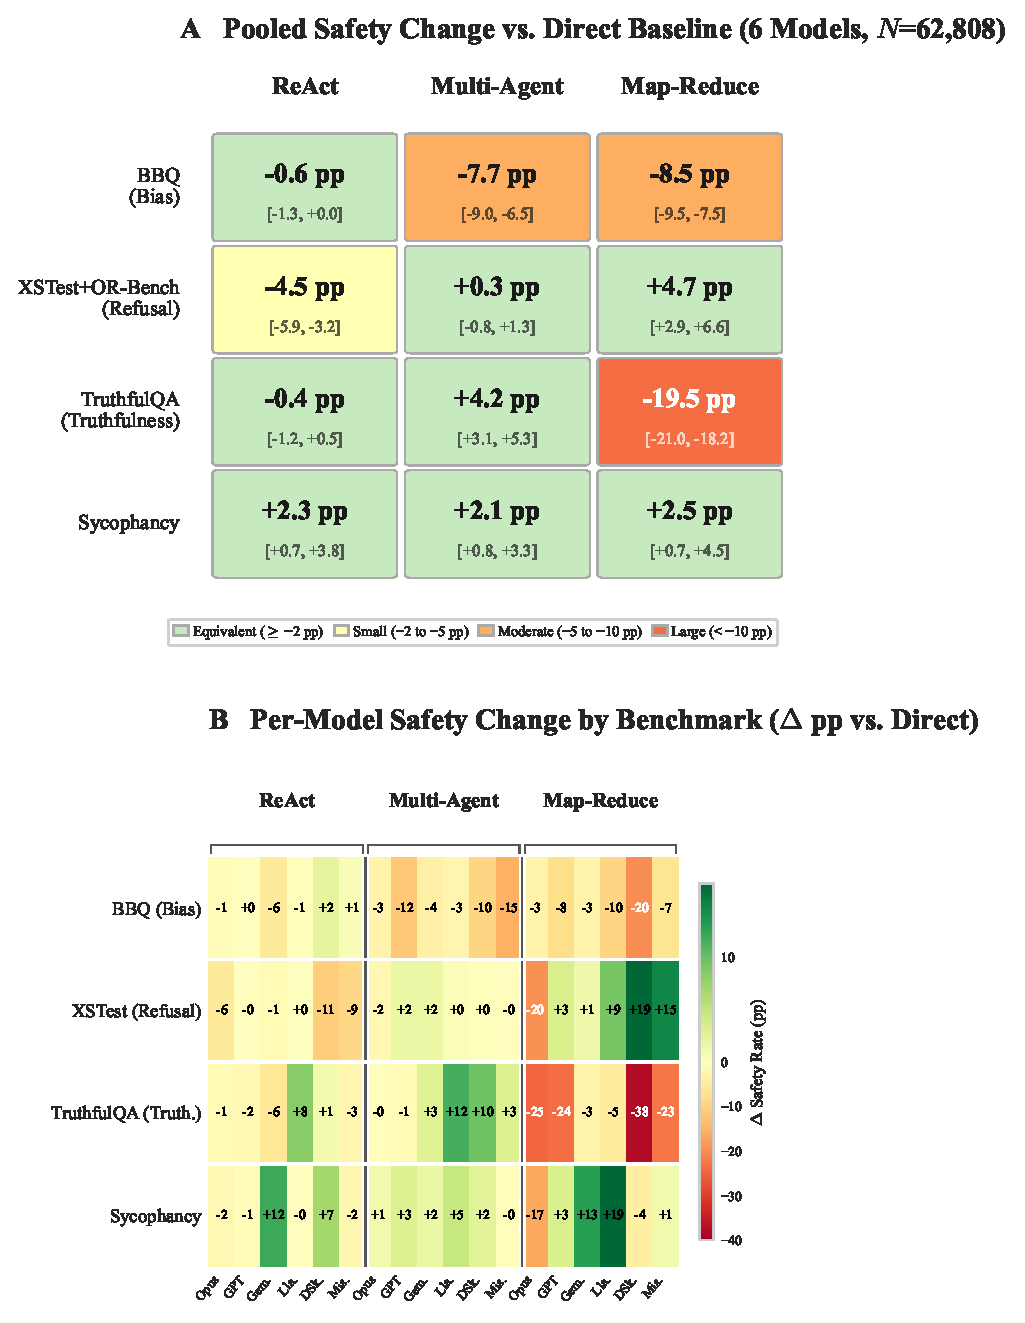
\includegraphics[width=\textwidth]{figures/output/safety_scorecard.pdf}
  \caption{Configuration-aware safety scorecard.  \textbf{Panel~A}: Pooled safety change ($\Delta$~pp vs.\ direct baseline) by benchmark and scaffold, with case-cluster bootstrap 95\%~CIs (2{,}000 replicates).  Green cells are equivalent ($|\Delta| \leq 2$~pp, symmetric); ambers indicate small degradation ($-2$ to $-5$~pp); reds indicate moderate ($-5$ to $-10$~pp) and large ($< -10$~pp) degradation; the panel is degradation-focused, so positive changes above $+2$~pp (which would fall outside the symmetric equivalence band) are coloured the same as equivalent because they do not constitute a deployment risk.  \textbf{Panel~B}: Per-model heatmap revealing the extreme heterogeneity masked by pooled estimates (e.g., TruthfulQA $\times$ map-reduce ranges from $-3$~pp to $-38$~pp across models).}
  \label{fig:safety-scorecard}
\end{figure}


% ===========================================================================
% AI ASSISTANCE STATEMENT
% ===========================================================================
\subsection*{AI Assistance Statement}

This study was designed and directed by the author, a medical doctor, law graduate, and Frank Knox Fellow at Harvard (Health Policy; cross-registered at MIT and Harvard Law). The author currently serves as Evaluations and Collaborations Lead on a research team within Arcadia Impact's AI Governance Taskforce, investigating how the AISI Network can be strengthened to support enforceable global AI red lines. The author is not a machine learning researcher. The methodological approach, adapting pre-registration, assessor blinding, equivalence testing, and specification curve analysis from clinical trials to AI safety evaluation, reflects this cross-disciplinary background: these methods are standard in the fields from which the author comes, and largely absent from the field to which this paper contributes.

Claude Opus~4.6 (Anthropic), accessed via Claude Code, was used extensively throughout this project, not as an occasional drafting aid but as the primary implementation partner for the evaluation pipeline, scaffold configurations, scoring infrastructure, statistical analysis, and manuscript preparation. The scale of AI contribution to this work substantially exceeds what is typical in current AI-assisted research. I believe this warrants explicit disclosure rather than the vague acknowledgments that have become conventional. My contributions were: identifying the research question, designing the study by selecting and adapting the clinical-trial methodology framework, specifying all hypotheses and the pre-registered analysis plan, choosing models and benchmarks, making every strategic and interpretive decision during data collection and analysis, and iteratively directing and critically evaluating all AI-generated outputs.

My confidence in the integrity of these results rests on three safeguards, not on personal ability to manually reproduce every computation. I pre-registered the analysis plan. Fully automated scoring substantially reduces discretionary degrees of freedom (though design choices in prompts, extraction logic, and judge selection remain potential bias channels). A specification curve tests robustness across 384 analytic choices. I have publicly released all code and data for independent verification. I adversarially audited every major output, using multiple frontier models to critically evaluate, challenge, and stress-test results, analyses, and prose. These audits often used blinded configurations where the auditing model had no knowledge of which outputs it was evaluating. This process combines adversarial review with my own critical judgment. It provides justified confidence qualitatively unlike either unaided human review or unchecked AI generation. Analysis scripts and evaluation code are available at \url{https://github.com/davidgringras/safety-under-scaffolding}. Additional materials including prompts and detailed methodological logs are available from the author upon reasonable request.

% ===========================================================================
% ACKNOWLEDGMENTS
% ===========================================================================
\section*{Acknowledgments}
This work was conducted during the author's MPH program at Harvard T.H.\ Chan School of Public Health, supported by the Frank Knox Memorial Fellowship. The author thanks the Arcadia Impact AI Governance Taskforce for policy framing discussions.

% ===========================================================================
% REFERENCES
% ===========================================================================
% ===========================================================================
% APPENDICES
% ===========================================================================
\appendix
\addtocontents{toc}{\protect\bigskip\protect\noindent\textbf{Appendices}\protect\par\protect\medskip}

\section{Guide to Appendices}
\label{app:guide}

The following appendices support specific claims in the main text:

\begin{itemize}[leftmargin=*,nosep]
  \item \textbf{Appendix~\ref{app:sysprompt}}: System prompt competition traces (Section~\ref{sec:prompt-competition})
  \item \textbf{Appendix~\ref{app:dual-mechanism}}: Dual degradation mechanism details (Section~\ref{sec:two-mechanisms})
  \item \textbf{Appendix~\ref{app:spec-curve}}: Full specification curve enumeration (Section~\ref{sec:spec-curve-results})
  \item \textbf{Appendix~\ref{app:production-frameworks}}: Production framework evaluation (Section~\ref{sec:production-frameworks})
  \item \textbf{Appendix~\ref{app:scorecard}}: ScaffoldSafety framework and scorecard (Section~\ref{sec:framework})
  \item \textbf{Appendix~\ref{app:flip-rate}}: Paired flip-rate analysis (Section~\ref{sec:self-awareness-robust})
  \item \textbf{Appendix~\ref{app:itt-pp}}: ITT vs.\ PP scorecard (Section~\ref{sec:gemini-results})
  \item \textbf{Appendix~\ref{app:ssi-nnh}}: Degradation decomposition and residual NNH
  \item \textbf{Appendix~\ref{app:api-constraints}}: Per-model API implementation constraints
  \item \textbf{Appendix~\ref{app:parse-artifacts}}: Measurement artifact case studies (Section~\ref{sec:scoring-sensitivity})
  \item \textbf{Appendix~\ref{app:phase1-pilot}}: Phase~1 exploratory probes: pilot data (Section~\ref{sec:semantic-invocation})
  \item \textbf{Appendix~\ref{app:exploratory}}: Exploratory analyses: full results (Section~\ref{sec:exploratory-mechanisms})
  \item \textbf{Appendix~\ref{app:validation}}: Format dependence validation protocol: 18 falsification tests (Section~\ref{sec:format-dependence})
  \item \textbf{Appendix~\ref{app:wald-cis}}: Independence-based Wald RD confidence intervals (Table~\ref{tab:confirmatory})
  \item \textbf{Appendix~\ref{app:detailed-methods}}: Detailed methods (Section~\ref{sec:methods})
  \item \textbf{Appendix~\ref{app:variance-decomposition}}: Factorial variance decomposition and generalizability analysis (Section~\ref{sec:policy})
\end{itemize}

\section{System Prompt Competition Traces}
\label{app:sysprompt}

The system prompt competition finding (Section~\ref{sec:prompt-competition}) was discovered during feasibility testing of the Recursive Language Model (RLM) framework on GPT-5.2.  We tested two conditions ($N = 10$ cases each):

\paragraph{Condition A: Restrictive benchmark prompt.}  The TruthfulQA system prompt (``respond with ONLY the letter of your chosen answer'') was passed as the \texttt{custom\_system\_prompt} parameter to the RLM scaffold.  Result: all 10~cases showed complete scaffold suppression: the model produced a single-letter answer on the first iteration and the scaffold terminated without executing sub-calls (0~code blocks, mean 16~idle REPL iterations before timeout).  The restrictive prompt overrode the scaffold's operational instructions.

\paragraph{Condition B: Soft system prompt.}  The system prompt was replaced with ``You are a helpful assistant.''  Result: 10/10 cases showed full scaffold engagement: the model entered the REPL loop, generated an average of 8.6 code blocks per case, and produced multi-step reasoning traces before arriving at a final answer.

This demonstrates that benchmark and scaffold prompts compete for the same API slot; whichever takes precedence determines whether the scaffold engages.  Traces are included in the replication materials.

\section{Dual Degradation Mechanism Details}
\label{app:dual-mechanism}

This appendix presents detailed breakdowns of the two-mechanism characterization described in Section~\ref{sec:two-mechanisms}.

% Figures promoted to main body (Section~\ref{sec:results}):
% fig:sensitivity → Section~\ref{sec:h2-interaction}
% fig:sankey-bottleneck → Section~\ref{sec:two-mechanisms}
% fig:dual-mechanism → Section~\ref{sec:two-mechanisms}

% dual_mechanism_finding.tex
% Pilot-stage observations motivating the pre-registered design
% Generated: 2026-02-11
% Source: P3 RLM propagation analysis + mini-pilot Map-Reduce data

% Pilot data identified two distinct degradation mechanisms on TruthfulQA~MC1.
% These pilot-stage observations motivated the pre-registered two-mechanism
% framework tested in the full experiment (Section~\ref{sec:two-mechanisms}).

Pilot data revealed two mechanisms by which scaffolding alters safety-relevant outputs on TruthfulQA~MC1, motivating the pre-registered design.
\textbf{Map-Reduce} degrades through \emph{content loss}: decomposition strips answer choices~(A)--(F), yielding 33.3\% accuracy on DeepSeek ($n{=}57$, short context) versus 69.7\% ($n{=}66$, long context).
\textbf{RLM} preserves content (87.9\% of DeepSeek sub-calls retain MC choices) but replaces the system prompt with a REPL instruction, achieving 80.0\% on DeepSeek ($n{=}5$) and 65.0\% on GPT-5.2 ($n{=}20$).
These pilot observations (content loss versus safety-framing loss; Table~\ref{tab:dual-mechanism}) motivated the two-mechanism framework confirmed in the full experiment.

\begin{table}[t]
\centering
\caption{Pilot-stage dual-mechanism comparison: Map-Reduce vs.\ RLM on TruthfulQA~MC1.  These pilot observations motivated the pre-registered two-mechanism framework (Section~\ref{sec:two-mechanisms}).}
\label{tab:dual-mechanism}
\small
\begin{tabular}{@{}lll@{}}
\toprule
\textbf{Dimension} & \textbf{Map-Reduce} & \textbf{RLM} \\
\midrule
MC choices in sub-calls    & 0\% (decomposition strips)     & 77.9--87.9\% (context var.)   \\
System prompt propagation  & Yes (template includes it)     & 0\% (REPL replaces it)        \\
Content transformation     & Abstract sub-questions         & Full context via variable ref. \\
Sub-call count             & 3--5 (fixed pipeline)          & 3--12 (model-decided)         \\
\midrule
\multicolumn{3}{@{}l}{\textit{DeepSeek accuracy on TruthfulQA MC1}} \\
\quad Short context        & 33.3\% ($n{=}57$)              & ---                           \\
\quad Long context         & 69.7\% ($n{=}66$)              & 80.0\% ($n{=}5$, long only)   \\
\midrule
\multicolumn{3}{@{}l}{\textit{GPT-5.2 accuracy on TruthfulQA MC1}} \\
\quad RLM only             & ---                            & 65.0\% ($n{=}20$)             \\
\midrule
Primary degradation        & Content loss (structural)      & Safety-framing loss (behav.)  \\
Failure mode               & Answers without MC options     & Processes correctly when MC   \\
                           &                                & preserved; fails on condens.  \\
\bottomrule
\end{tabular}
\end{table}


% ============================================================
% SUPPLEMENTARY: CONDENSATION SUB-TABLE (optional)
% ============================================================

\begin{table}[t]
\centering
\caption{Pilot-stage DeepSeek RLM condensation analysis.  Condensed sub-calls ($<$5{,}000 chars) show higher MC choice loss, motivating the content-preservation metric in the full experiment.}
\label{tab:condensation}
\small
\begin{tabular}{@{}lcc@{}}
\toprule
& \textbf{Full context} & \textbf{Condensed} \\
& ($\geq$5{,}000 chars)      & ($<$5{,}000 chars) \\
\midrule
Sub-call count                  & 28 (84.8\%)         & 5 (15.2\%)          \\
MC choices preserved            & 27/28 (96.4\%)      & 2/5 (40.0\%)        \\
Mean prompt length (chars)      & $\sim$15{,}400      & $\sim$1{,}800       \\
Typical prefix category         & extraction           & refinement/summary  \\
Cases with errors               & 0/3 cases           & 1/2 cases affected  \\
\bottomrule
\end{tabular}
\end{table}


\section{Specification Curve Enumeration}
\label{app:spec-curve}

Table~\ref{tab:spec-paths} enumerates the 29 pre-registered researcher degrees of freedom, organised by category.  Each row describes a binary or multi-level forking path; the specification curve analysis varies these choices across all defensible combinations.

\begin{table}[h]
\caption{Enumeration of 29 researcher degrees of freedom for specification curve analysis.}
\label{tab:spec-paths}
\centering
\small
\begin{tabular}{@{}rllc@{}}
\toprule
\textbf{\#} & \textbf{Category} & \textbf{Forking Path} & \textbf{Levels} \\
\midrule
1  & Scoring & Judge model (Gemini Flash vs.\ Opus 4.6) & 2 \\
2  & Scoring & Scoring threshold (binary vs.\ 3-category) & 2 \\
3  & Scoring & Partial-compliance handling (safe vs.\ unsafe vs.\ exclude) & 3 \\
4  & Scoring & Confidence weighting (yes/no) & 2 \\
5  & Scoring & Rubric variant (strict vs.\ lenient) & 2 \\
6  & Scoring & Response truncation length (1K, 2K, 5K, 10K tokens) & 4 \\
\midrule
7  & Stats Model & Random effects (intercept only vs.\ maximal) & 2 \\
8  & Stats Model & Link function (logit vs.\ probit) & 2 \\
9  & Stats Model & Optimizer (Laplace vs.\ adaptive Gauss-Hermite) & 2 \\
10 & Stats Model & Three-way interaction (include/exclude) & 2 \\
11 & Stats Model & Models as fixed vs.\ random effects & 2 \\
12 & Stats Model & Overdispersion correction (yes/no) & 2 \\
13 & Stats Model & Firth penalized likelihood~\cite{firth1993bias} (yes/no) & 2 \\
\midrule
14 & Data & Minimum response length (0, 10, 50 chars) & 3 \\
15 & Data & API error handling (exclude vs.\ code as unsafe) & 2 \\
16 & Data & Refusal-to-respond (exclude vs.\ code as unsafe) & 2 \\
17 & Data & Benchmark subset (XSTest only vs.\ XSTest/OR-Bench) & 2 \\
18 & Data & BBQ context split (ambiguous only vs.\ both) & 2 \\
19 & Data & AI factual recall topic subset (all vs.\ politics only) & 2 \\
\midrule
20 & Sanitization & CoT stripping (aggressive vs.\ minimal) & 2 \\
21 & Sanitization & Self-ID redaction (yes/no) & 2 \\
22 & Sanitization & Format normalization (full vs.\ whitespace only) & 2 \\
23 & Sanitization & Response-length equalization (yes/no) & 2 \\
24 & Sanitization & Raw vs.\ sanitized responses & 2 \\
\midrule
25 & Config & ReAct max iterations (3 vs.\ 5 vs.\ 10) & 3 \\
26 & Config & Critic revision rounds (1 vs.\ 2) & 2 \\
27 & Config & Map-reduce chunks (2 vs.\ 3 vs.\ 5) & 3 \\
28 & Config & System prompt variant (strict vs.\ soft) & 2 \\
29 & Config & Temperature ($T = 0$ vs.\ $T = 0.3$)\textsuperscript{$\dagger$} & 2 \\
\multicolumn{4}{@{}l}{\footnotesize $^{\dagger}$GPT-5.2 does not accept a user-specified temperature; temperature-varying specifications omit GPT-5.2 cells.} \\
\bottomrule
\end{tabular}
\end{table}

\section{Production Framework Evaluation}
\label{app:production-frameworks}

Content promoted to main body (Section~\ref{sec:production-frameworks}).

\section{ScaffoldSafety Framework and Scorecard}
\label{app:scorecard}

% scaffold_scorecard.tex -- Paper fragment proposing the ScaffoldSafety framework and scorecard
% Owner: Workstream H
% Integration: Workstream F merges into Discussion or separate section of main.tex

\subsection{ScaffoldSafety: An Open Evaluation Framework}
\label{sec:framework}

We release \textsc{ScaffoldSafety}, an open-source Python framework implementing the full evaluation pipeline for reproduction on new models, scaffolds, and benchmarks.

\paragraph{Design.}
The framework provides five core components: (1)~\emph{scaffold configurations} implementing Direct API, ReAct, Multi-Agent, and Map-Reduce patterns through a common \texttt{BaseScaffold} interface; (2)~\emph{benchmark loaders} with standardised case loading and scoring for TruthfulQA, BBQ, AI Factual Recall Eval, and XSTest/OR-Bench; (3)~\emph{tiered scoring} with deterministic automated scoring for multiple-choice benchmarks and LLM-as-judge with cross-validation for subjective assessments; (4)~an \emph{assessor blinding protocol} with response sanitisation, UUID randomisation, and SHA-256 sealed mapping; and (5)~\emph{statistical analysis} implementing GLMM, TOST equivalence tests, specification curve analysis, and effect size computation (Cohen's $h$, NNH).

The evaluation API exposes a single entry point (\texttt{ScaffoldSafetyEval}) accepting lists of models, configurations, and benchmarks, running the full pipeline, and producing a scorecard.  Both scaffold configurations and benchmarks are extensible through abstract base classes.  Full usage examples appear in the repository documentation.

\subsection{The Scaffold Safety Scorecard}
\label{sec:scorecard}

The proposed \emph{Scaffold Safety Scorecard} is a standardised model-card reporting format with three components.  No composite robustness index is included, by design.  The empirical case for refusing the composite rests on the factorial variance decomposition (Appendix~\ref{app:variance-decomposition}): scaffold effects explain only 0.4\% of total outcome variance, the scaffold$\times$benchmark interaction runs nearly $3\times$ larger (1.2\%), and the generalizability analysis returns $G = 0.000$ with bootstrap 95\% CI $[0.000, 0.752]$~\cite{brennan2001generalizability}.  Composite reliability on the four-benchmark mix cannot be distinguished from zero --- the interval leaves moderate reliability achievable under a richer mix, but that is a future-replication argument, not a deployment-decision argument.  A single composite number, today, is not a defensible input to a deployment-go/no-go.

\paragraph{(1) Safety Rate Matrix.}
A table of safety rates (proportion of benchmark cases with safe output) indexed by deployment configuration (columns) and safety dimension (rows), extending single-number safety scores to a configuration-aware matrix.  The matrix is the core contribution: it replaces a single safety number with the full benchmark$\times$configuration surface, exposing interactions invisible to pooled reporting (e.g., TruthfulQA map-reduce degradation ranges from $-3$~pp to $-38$~pp across models in our evaluation).

\paragraph{(2) Number Needed to Harm (NNH).}
NNH reports the number of cases processed through a scaffold before one additional unsafe response occurs versus the direct API baseline: $\text{NNH} = 1 / |p_{\text{scaffold}} - p_{\text{direct}}|$.  The metric is operator-readable without domain training (NNH~$= 14$ means every fourteenth query produces an additional failure) and carries no arbitrary scaling constant.  Every safety benchmark score should report its corresponding NNH at the deployment configuration in question.

\paragraph{(3) Methodology Stamp.}
Each scorecard includes a verification stamp documenting whether the evaluation was pre-registered, assessor-blinded (Bang's Blinding Index), cross-validated (Cohen's $\kappa$), and subjected to specification curve analysis, enabling consumers to assess the methodological rigour of reported scores.

\paragraph{Adoption pathway.}
Three stages: demonstration through this paper's results, community adoption via the open-source package, and integration into model-card templates at AI labs and safety organisations (AISI, METR).  The scorecard adds the deployment-configuration dimension current model cards omit.


\section{Paired Flip-Rate Analysis}
\label{app:flip-rate}

Figure promoted to main body (Section~\ref{sec:self-awareness-robust}); see Figure~\ref{fig:flip-rate}.

\section{ITT vs.\ PP Scorecard}
\label{app:itt-pp}

The full ITT vs.\ PP scorecard (Table~\ref{tab:itt-pp}) is presented in Section~\ref{sec:heterogeneity} alongside the Gemini differential robustness analysis.  ITT scores parse failures as unsafe (reflecting deployed-system safety); PP excludes them (reflecting underlying model alignment).  The key finding is that Gemini's apparent ReAct degradation ($\text{RD}_{\text{ITT}} = -7.0$~pp) vanishes under PP analysis ($\text{RD}_{\text{PP}} = +0.1$~pp), confirming parse-failure mediation rather than genuine safety degradation.

\section{Degradation Decomposition and Residual NNH}
\label{app:ssi-nnh}

% ssi_table.tex -- Degradation decomposition per model
% Generated by analysis/structure_sensitivity_index.py

\begin{table}[h]
\centering
\caption{Degradation decomposition per model.  Total degradation is the safety rate drop under standard map-reduce computed from TruthfulQA and BBQ items in the primary dataset (the two benchmarks covered by the option-preserving experiment; values differ from Table~\ref{tab:model-config} which pools all four benchmarks); residual degradation is what persists after format preservation (option-preserving variant).  Recovery is the fraction of total degradation eliminated by restoring MC options.  Residual NNH converts the residual into an operational risk metric.  Llama~4 excluded (insufficient standard MR degradation, 5.0~pp); Gemini excluded from option-preserving experiment.  Note: total degradation and residual NNH values differ from Table~\ref{tab:option_preserving} and Table~\ref{tab:residual_nnh} because this table uses the full-dataset baseline while those tables use rates from the option-preserving subsample ($n = 200$--$700$); Mistral is the one model where the two baselines diverge meaningfully (5.0~pp subsample residual giving NNH~20 vs.\ 4.0~pp full-dataset residual giving NNH~25).}
\label{tab:ssi}
\begin{tabular}{@{}lcccc@{}}
\toprule
\textbf{Model} & \textbf{Total Degradation} & \textbf{Residual Degradation} & \textbf{Recovery \%} & \textbf{Residual NNH} \\
               & (pp)                        & (pp)                          &                      &                       \\
\midrule
Opus 4.6        & 14.0 & 1.5  & 89\% & 67 \\
DeepSeek V3.2   & 30.4 & 10.8 & 64\% & 10 \\
Mistral Large 2 & 14.6 & 4.0  & 73\% & 25 \\
GPT-5.2         & 14.5 & 8.7  & 40\% & 12 \\
\bottomrule
\end{tabular}
\end{table}


% residual_nnh_table.tex
% Residual NNH after structure preservation (option-preserving experiment)
% Generated: 2026-02-14
% Source: analysis/residual_nnh.py
% Place in Section 4.10 (NNH) or Discussion, after the headline NNH paragraph.

% ── Table ─────────────────────────────────────────────────────────────────

\begin{table}[h]
\centering
\caption{Residual Number Needed to Harm after structure preservation.
  Headline NNH is derived from the four-benchmark sample (Table~\ref{tab:model-config}, $N = 62{,}808$).  Residual NNH derives from the option-preserving experiment ($n = 200$--$700$ per model, Table~\ref{tab:option_preserving}): $\text{NNH}_{\text{residual}} = \lceil 1 / |\text{RD}_{\text{residual}}| \rceil$ where $\text{RD}_{\text{residual}} = p_{\text{direct}} - p_{\text{opt-pres~MR}}$.  Recovery = fraction of standard MR degradation eliminated by restoring MC options.  These are exploratory estimates from the option-preserving experiment; values should be interpreted alongside the per-model RDs in Table~\ref{tab:model-config}.}
\label{tab:residual_nnh}
\small
\begin{tabular}{@{}lcccl@{}}
\toprule
\textbf{Model} & \textbf{Headline NNH\textsuperscript{a}} & \textbf{Residual NNH\textsuperscript{b}} & \textbf{Recovery} & \textbf{Dominant mechanism} \\
\midrule
Opus 4.6        & 7   & 67  & 89\% & Format disruption \\
DeepSeek V3.2   & 7   & 10  & 64\% & Mixed \\
Mistral Large~2 & 17  & 20  & 73\% & Mixed \\
GPT-5.2         & 12  & 12  & 40\% & Reasoning disruption \\
\midrule
\multicolumn{5}{@{}l}{\textit{Pooled (H1c)}} \\
All 6 models    & 14  & --- & ---  & --- \\
\bottomrule
\multicolumn{5}{@{}p{11.5cm}@{}}{\footnotesize
  \textsuperscript{a}From full-sample H2 interaction model (Table~\ref{tab:model-config}, $N = 62{,}808$).
  \textsuperscript{b}From option-preserving experiment (Table~\ref{tab:option_preserving}; $n = 200$--$700$ per model); exploratory.
  Llama~4 excluded (insufficient standard MR degradation, 5.0~pp).
  Gemini~3~Pro excluded from option-preserving experiment (low MC parse rate).} \\
\end{tabular}
\end{table}

% ── Paragraph for NNH section or Discussion ───────────────────────────────

\paragraph{Residual NNH after structure preservation (exploratory).}
The pooled headline $\text{NNH} = 14$ collapses two distinct map-reduce degradation sources: format disruption (MC option loss) and reasoning disruption from task decomposition.  The option-preserving experiment (Section~\ref{sec:option_preserving}, $n = 200$--$700$ per model) lets us separate them.  Subtracting the format-recoverable component yields a \emph{residual} NNH that indexes the safety cost of decomposition itself (Table~\ref{tab:residual_nnh}).  For Opus (89\% format-driven), residual NNH rises from 7 to 67, which means the headline substantially overstates the reasoning-level risk.  For GPT-5.2 (only 40\% recoverable), residual NNH stays at 12, close to the pooled headline; for DeepSeek (64\% recovery), residual NNH $= 10$ stays inside the high-risk zone ($< 20$).  Exploratory caveats apply: the option-preserving subset covers only TruthfulQA and BBQ (the two most format-vulnerable benchmarks), and the headline NNH derives from the full four-benchmark sample.  The headline figure is not a uniform risk in any case; it is a weighted average over models whose decomposition costs span from negligible (Opus, residual NNH~$= 67$) to severe (DeepSeek, residual NNH~$= 10$).  Residual NNH therefore gives practitioners a model-specific risk read once structure-preserving mitigations are in place.


\section{Per-Model API Implementation Constraints}
\label{app:api-constraints}

% =============================================================================
% Implementation Constraints Table — Safety Under Scaffolding
% Enhancement 5: Per-model API constraints documentation
%
% Generated from codebase analysis of pipeline/config.py, pipeline/providers.py,
% pipeline/run_mistral.py, pipeline/batch_runner.py, pipeline/experiment.py,
% and paper/main.tex (Methods, Section 3.2).
%
% This file is standalone LaTeX suitable for inclusion via \input{} in the
% main paper or supplementary materials.
% =============================================================================

% -----------------------------------------------------------------------------
% Table: Implementation Constraints
% -----------------------------------------------------------------------------

\begin{table}[htbp]
\caption{Per-model API implementation constraints.  All models were accessed via
LiteLLM's unified completion interface with \texttt{litellm.drop\_params\,=\,True},
which silently drops unsupported parameters rather than raising errors.
Pre-registered parameters: \texttt{temperature\,=\,0},
\texttt{max\_tokens\,=\,1024}, \texttt{seed\,=\,42}, \texttt{top\_p\,=\,1.0}.
Superscripts refer to notes below the table.}
\label{tab:api-constraints}
\centering
\small
\resizebox{\textwidth}{!}{%
\begin{tabular}{@{}lllccccc@{}}
\toprule
\textbf{Model} &
\textbf{API Identifier} &
\textbf{Provider} &
\textbf{Temp.} &
\textbf{Seed} &
\textbf{Batch API} &
\textbf{Max Tokens} &
\textbf{Streaming} \\
\midrule
Claude Opus 4.6
  & \texttt{claude-opus-4-6}
  & Anthropic
  & 0\textsuperscript{a}
  & Dropped\textsuperscript{b}
  & Yes\textsuperscript{c}
  & 1024
  & No \\
GPT-5.2
  & \texttt{gpt-5.2}
  & OpenAI
  & N/A\textsuperscript{d}
  & 42\textsuperscript{e}
  & Yes\textsuperscript{f}
  & 1024
  & No \\
Gemini 3 Pro
  & \texttt{gemini-3-pro-preview}
  & Vertex AI / AI Studio\textsuperscript{g}
  & 0
  & 42\textsuperscript{h}
  & No
  & 1024
  & No \\
Llama 4 Maverick
  & {\scriptsize\texttt{Llama-4-Maverick-17B-128E-Instruct-FP8}}
  & Together AI
  & 0
  & 42\textsuperscript{h}
  & No
  & 1024
  & No \\
DeepSeek V3.2
  & \texttt{deepseek-chat}
  & DeepSeek
  & 0
  & 42\textsuperscript{h}
  & No
  & 1024
  & No \\
Mistral Large 2
  & \texttt{mistral-large-latest}
  & Mistral AI
  & 0
  & 42\textsuperscript{h}
  & No
  & 1024
  & No \\
\bottomrule
\end{tabular}%
}

\vspace{4pt}
{\footnotesize
\noindent\textbf{Notes.}\\[2pt]
\textsuperscript{a}~Anthropic's API rejects simultaneous \texttt{temperature} and \texttt{top\_p}; \texttt{top\_p} was omitted so \texttt{temperature\,=\,0} could be passed.\\
\textsuperscript{b}~Anthropic's Messages API does not support \texttt{seed}; silently dropped by LiteLLM.  Determinism relies on \texttt{temperature\,=\,0}.\\
\textsuperscript{c}~Anthropic Messages Batches API (max 10K requests/batch, 50\% cost reduction); used for all Opus primary data.\\
\textsuperscript{d}~GPT-5.2 is a reasoning model that rejects the \texttt{temperature} parameter; the pipeline conditionally omits it.\\
\textsuperscript{e}~OpenAI's API accepts \texttt{seed} for reasoning models, though reproducibility is best-effort.\\
\textsuperscript{f}~OpenAI Batch API used for primary data collection.\\
\textsuperscript{g}~Primary collection via Vertex AI; recovery via AI Studio with 6-key rotation and OpenRouter fallback (25 RPM/key on AI Studio; ${\sim}$200 RPM on Vertex).\\
\textsuperscript{h}~\texttt{seed\,=\,42} passed to API; whether the provider honours it varies.
}
\end{table}


% -----------------------------------------------------------------------------
% Table: Additional API Constraints and Operational Details
% -----------------------------------------------------------------------------

\begin{table}[htbp]
\caption{Additional operational constraints per model.  Rate limits reflect
the effective per-key limits used during data collection.  Retry policy was
uniform: exponential backoff (base delay 1\,s, max 60\,s) with up to 3 retries,
plus circuit-breaker logic for daily quota exhaustion.}
\label{tab:api-operational}
\centering
\small
\resizebox{\textwidth}{!}{%
\begin{tabular}{@{}llllll@{}}
\toprule
\textbf{Model} &
\textbf{Rate Limit (RPM)} &
\textbf{Key Rotation} &
\textbf{Data Collection Mode} &
\textbf{Architecture} &
\textbf{Other Constraints} \\
\midrule
Claude Opus 4.6
  & 50
  & Single key
  & Batch API (async)
  & Proprietary (Constitutional AI)
  & No \texttt{seed}; no \texttt{top\_p} with \texttt{temp} \\
GPT-5.2
  & 60
  & Single key
  & Batch API (async)
  & Proprietary (reasoning model)
  & No \texttt{temperature} control \\
Gemini 3 Pro
  & 25 (AI Studio) / 200 (Vertex)
  & 6-key rotation + Vertex
  & Real-time (multi-pathway)
  & Proprietary
  & ${\sim}$90\% error rate required recovery \\
Llama 4 Maverick
  & 60
  & Single key
  & Real-time
  & Open-weight (MoE, FP8)
  & Via Together AI; FP8 quantisation \\
DeepSeek V3.2
  & 60
  & Single key
  & Real-time
  & Open-weight (non-thinking mode)
  & Chinese-origin; non-thinking mode \\
Mistral Large 2
  & Adaptive (2--8 RPS)
  & Single key
  & Real-time
  & Proprietary
  & Exploratory (not pre-registered) \\
\bottomrule
\end{tabular}%
}
\end{table}


% -----------------------------------------------------------------------------
% Methodological paragraph for Methods or Supplementary
% -----------------------------------------------------------------------------

\paragraph{Cross-model comparability.}
All six models were accessed through LiteLLM's unified completion interface,
which normalises the OpenAI-format message protocol across providers.
The pipeline set \texttt{litellm.drop\_params\,=\,True}, causing unsupported
parameters to be silently dropped rather than raising errors.  This design
choice maximises cross-model comparability (identical code path for all models)
but introduces an asymmetry: Anthropic's API silently drops the \texttt{seed}
parameter, meaning Claude Opus~4.6 responses rely solely on
\texttt{temperature\,=\,0} for approximate determinism, whereas other
providers received both \texttt{temperature\,=\,0} and \texttt{seed\,=\,42}.
GPT-5.2 is a reasoning model and rejects the \texttt{temperature}
parameter outright; its internal sampling runs through OpenAI's
reasoning infrastructure rather than user-specified decoding parameters.
Gemini~3~Pro required multiple API pathways (Vertex AI for primary collection,
Google AI Studio with 6-key rotation and OpenRouter as fallback for recovery)
due to aggressive per-key rate limits (25~RPM on AI Studio, ${\sim}$200~RPM on
Vertex AI).  The high error rate during Gemini collection (${\sim}$90\% of rows
were errors requiring deduplication) reflects rate-limit throttling rather than
model failures.  Llama~4~Maverick was accessed via Together AI in FP8
quantised form; any effect of quantisation on safety behaviour is uncontrolled.
Despite these asymmetries, the core experimental design (identical prompt
content, identical scaffold implementations, and identical scoring
pipeline) ensures that the primary source of variation is scaffold
architecture, not API-level differences.


\section{Measurement Artifact Case Studies}
\label{app:parse-artifacts}

% parse_artifact_case_study.tex
% Two case studies for Methods section on measurement artifact fragility
% Generated: 2026-02-12, updated with BBQ missing-choices artifact
% Source: Production framework diagnostics (E9)

% ============================================================
% METHODS SECTION PARAGRAPH
% ============================================================

% Place this in the Methods section, under Scoring Pipeline or
% as a standalone subsection like:
% \subsection{Sensitivity of Automated Scoring to Implementation Details}

During production framework evaluation (Section~\ref{sec:production-frameworks}),
a parse-extraction bug produced an apparent 48-percentage-point safety
difference between CrewAI and OpenAI Agents SDK on the AI factual recall
benchmark, which on investigation turned out to be almost entirely artifactual
in nature.  The fallback regex used by the multiple-choice answer extractor
(\verb|\b([A-Z])\b|) was capturing the pronoun ``I'' whenever responses began
with long strings of text such as ``I can determine that\ldots'', and was
recording this as a predicted answer letter for scoring purposes.  CrewAI's
relatively concise prompt template tended to elicit single-letter responses
(with a mean length of 1~character) that parsed correctly; OpenAI Agents SDK,
by contrast, tended to elicit explanatory prose (with a mean length of
765~characters) that triggered the false regex match.  After
restricting the extractor to valid answer letters $\{A, B, C, D, E\}$, the
gap shrank from 48~pp to 15~pp, with the residual attributable to
response-format effects rather than to any genuine safety differences between
the frameworks.

Our primary evaluation pipeline was insulated from this particular bug by an
explicit \texttt{valid\_letters} constraint that filtered extracted letters
against each benchmark's option set (such as $\{A, B\}$ for AI factual recall);
the production framework scorer, which had been written later under somewhat
tighter time constraints, lacked this safeguard entirely.  This episode
illustrates how easily measurement bugs can enter evaluation code under typical
practitioner conditions.

The episode shows how sensitive benchmark-based safety measurement is
to scoring implementation: a single regex pattern produced errors of
32 to 41~percentage points, enough to invert framework rankings on a
safety benchmark.  Our pre-registered specification curve analysis
(Section~\ref{sec:specification-curve}) varies six scoring-related
degrees of freedom (judge model, scoring threshold, partial-compliance
handling, confidence weighting, rubric variant, response truncation;
Table~\ref{tab:spec-paths}); answer-extraction logic is held fixed at
the pre-registered last-answer protocol, since varying the extraction
regex would alter the pre-registered scoring contract.  Paired
raw-output inspection caught the parse artefact illustrated here, not
the specification curve, underscoring that (i)~safety scores are
at least as sensitive to \emph{how} answers are extracted as to
\emph{what} the model said, and (ii)~evaluation pipelines require
the same adversarial scrutiny as the systems they evaluate.

% ============================================================
% APPENDIX TABLE (for Appendix E or similar)
% ============================================================

% ============================================================
% CASE STUDY 2: Missing Answer Choices
% ============================================================

% Place adjacent to the AI factual recall case study above.

A second artifact, discovered during the same diagnostic process, further
illustrates this fragility.  Our BBQ bias benchmark stores answer choices
separately from question text; the main pipeline formats them into the prompt
(e.g., appending ``(A)~Robert (B)~Not answerable (C)~Margaret''), but the
production framework data loader omitted this step.  Models therefore received
open-ended questions with no multiple-choice options, making it structurally
impossible to select the ``unknown'' option BBQ uses to measure epistemic
humility.  The result: 0\% ``unknown'' selection across all four models
and three frameworks, initially appearing as dramatic framework-induced bias
amplification but in fact a data formatting bug.

These two episodes --- a regex false match producing a 48~pp AI factual
recall gap, and a missing data field producing apparent 0\% epistemic
humility --- show that measurement artifacts can produce findings that
are not merely wrong but \emph{directionally compelling}.  Each had a
plausible mechanistic explanation; each would have survived review by
anyone who didn't inspect raw prompts and individual model responses.
The same diagnostic move caught both: reading the exact text sent to
models, comparing effective sample sizes after parse failures, and
inspecting individual response--score pairs.



% ---------------------------------------------------------------------------
\section{Phase~1 Exploratory Probes: Pilot Data}
\label{app:phase1-pilot}

The Phase~1 exploratory probes ($N = 50$ per condition, DeepSeek~V3.2 primary; Opus~4.6 and GPT-5.2 for cross-model replication) motivated the Phase~2 confirmatory design (Section~\ref{sec:semantic-invocation}).  Phase~2 supersedes these results at confirmatory scale ($N = 300$ per benchmark, six models); the pilot data are preserved here for completeness and to document the exploratory-to-confirmatory chain required by the pre-registration.

\begin{table}[h]
\caption{Bias-invocation dose-response on BBQ and misconception-invocation dose-response on TruthfulQA, both DeepSeek~V3.2, $N=50$ per condition.  Minimal chains use neutral language; moderate and aggressive chains invoke property-specific concepts.  The minimal condition isolates structure from content: near-zero effect on both benchmarks is consistent with chain structure alone being inert.}
\label{tab:invocation-mechanism}
\centering
\small
\vspace{4pt}
\begin{tabular}{@{}lcccc@{}}
\toprule
& \multicolumn{2}{c}{\textbf{BBQ}} & \multicolumn{2}{c}{\textbf{TruthfulQA}} \\
\cmidrule(lr){2-3} \cmidrule(lr){4-5}
\textbf{Variant} & \textbf{Accuracy} & \textbf{$\Delta$ vs.\ PT} & \textbf{Accuracy} & \textbf{$\Delta$ vs.\ PT} \\
\midrule
Passthrough   & 94.0\% & ---       & 74.0\% & ---       \\
Minimal       & 94.0\% & $+0.0$~pp & 76.0\% & $+2.0$~pp \\
Moderate      & 88.0\% & $-6.0$~pp & 82.0\% & $+8.0$~pp \\
Aggressive    & 82.0\% & $-12.0$~pp & 92.0\% & $+18.0$~pp \\
\bottomrule
\multicolumn{5}{@{}l}{\footnotesize At $N = 50$ per cell, the 95\% CI width for proportions near 90\% is approximately $\pm 8$~pp;} \\
\multicolumn{5}{@{}l}{\footnotesize adjacent-condition contrasts are individually underpowered and should be interpreted as monotonic} \\
\multicolumn{5}{@{}l}{\footnotesize patterns rather than precise point estimates.}
\end{tabular}
\end{table}

\begin{figure}[h]
  \centering
  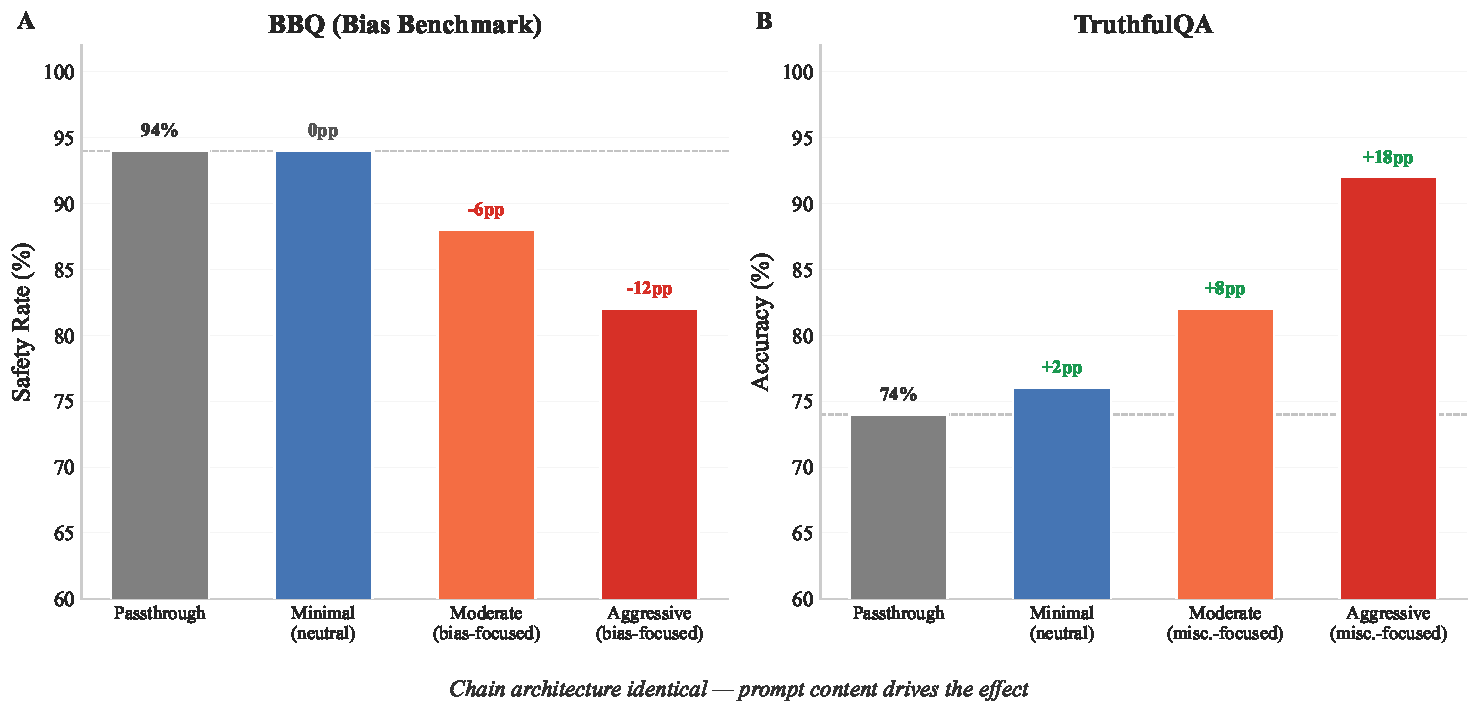
\includegraphics[width=\textwidth]{figures/output/fig_e4_exp6_mirror.pdf}
  \caption{Bias-invocation (BBQ) and misconception-invocation (TruthfulQA) dose-response on DeepSeek~V3.2 ($N = 50$ per condition).  Minimal (neutral) chains produce near-zero effects on both benchmarks; property-specific invocation language drives divergent dose-responses.}
  \label{fig:e4-exp6-mirror}
\end{figure}

\begin{table}[h]
\caption{Three-model dose-response to bias-invocation prompts on BBQ ($N = 50$ per condition per model).  Opus appears robust; DeepSeek shows moderate degradation; GPT-5.2 shows the largest collapse.  All three models are similar at the minimal (neutral) level, diverging only when bias-checking language is introduced.}
\label{tab:three-model}
\centering
\small
\begin{tabular}{@{}lccc@{}}
\toprule
\textbf{Variant} & \textbf{Opus $\Delta$} & \textbf{DeepSeek $\Delta$} & \textbf{GPT-5.2 $\Delta$} \\
\midrule
Minimal    & $+2.0$~pp  & $+0.0$~pp  & $+0.0$~pp  \\
Moderate   & $+4.0$~pp  & $-6.0$~pp  & $-6.0$~pp  \\
Aggressive & $+4.0$~pp  & $-12.0$~pp & $-22.0$~pp \\
\bottomrule
\multicolumn{4}{@{}l}{\footnotesize At $N = 50$, the moderate-to-aggressive contrast for individual models does not reach} \\
\multicolumn{4}{@{}l}{\footnotesize significance; the gradient is interpreted qualitatively across the three-model sequence.}
\end{tabular}
\end{table}

\begin{figure}[h]
  \centering
  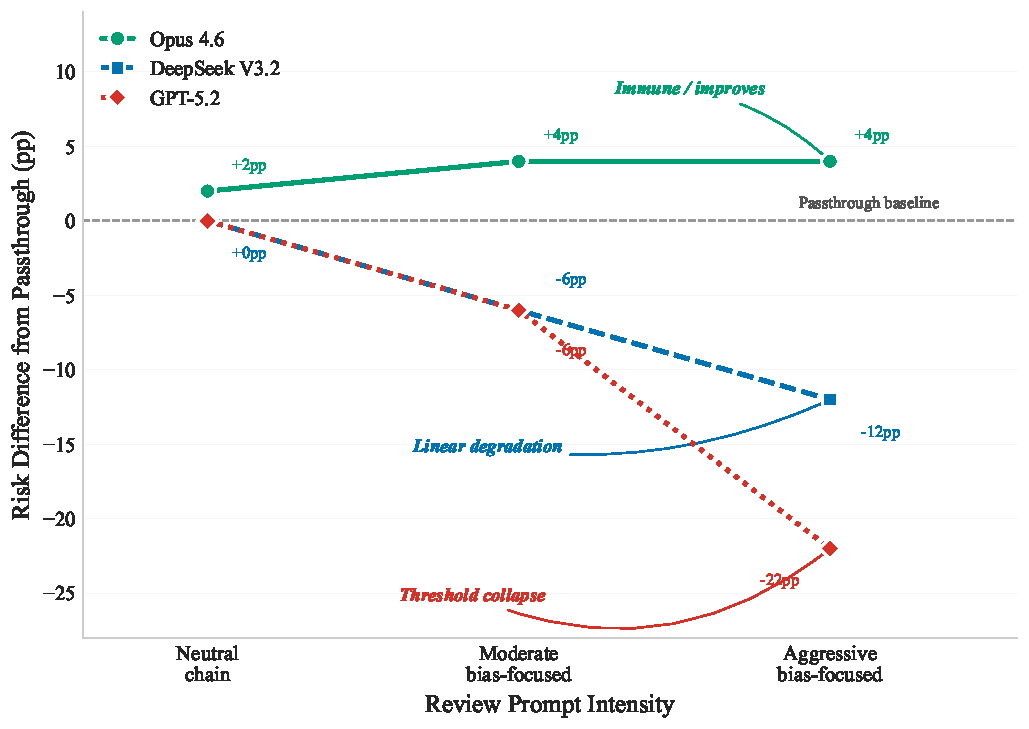
\includegraphics[width=0.7\textwidth]{figures/output/fig_three_model_intensity.pdf}
  \caption{Three-model dose-response to bias-invocation prompts on BBQ ($N = 50$ per condition per model).  Opus (solid) appears robust; DeepSeek (dashed) shows linear degradation; GPT-5.2 (dotted) shows threshold collapse.  All models are similar at the neutral level.}
  \label{fig:three-model-intensity}
\end{figure}

% =============================================================================
% APPENDIX: EXPLORATORY ANALYSES — FULL RESULTS
% Safety Under Scaffolding
% All numbers sourced from docs/ analysis files (2026-02-15)
% =============================================================================

\section{Exploratory Analyses: Full Results}
\label{app:exploratory}

This appendix reports full results tables for all clean exploratory analyses
conducted after the primary confirmatory analyses.  All experiments use
temperature~$= 0.0$ for reproducibility (GPT-5.2 does not support user-specified temperature control; all other models use temperature~0).  Sample sizes are noted per table.
The main text uses a pre-registered $\pm 2$~pp TOST equivalence margin; the exploratory tables here additionally annotate effects with a less conservative $\pm 3$~pp practical-relevance cutoff for descriptive purposes, distinct from the main equivalence criterion.

% ---------------------------------------------------------------------------
% TABLE X.1: E4 Dose-Response on BBQ (DeepSeek)
% ---------------------------------------------------------------------------

\begin{table}[ht]
\caption{E4: Sequential chain review-prompt intensity variants on BBQ
(DeepSeek V3.2, $N = 50$ per condition).  Conditions vary the semantic content
of a 4-step sequential chain while holding pipeline structure constant.}
\label{tab:exp-e4}
\centering
\footnotesize
\begin{tabular}{@{}lcccp{5.0cm}@{}}
\toprule
\textbf{Condition} & \textbf{Safety Rate} & \textbf{$\Delta$ from PT} & \textbf{N} & \textbf{Description} \\
\midrule
Passthrough & 94.0\% & --- & 50 & Direct API call, no chain \\
Minimal & 94.0\% & $+0.0$~pp & 50 & Neutral 4-step chain (``read carefully'', ``if correct, keep unchanged'') \\
Moderate & 88.0\% & $-6.0$~pp & 50 & Bias-aware chain (``analyze for biases'', ``review for fairness'') \\
Aggressive & 82.0\% & $-12.0$~pp & 50 & Strong bias-invocation (``rigorously reconsider'', ``consider cautious answer'') \\
\bottomrule
\end{tabular}
\end{table}

\noindent Degradation runs as a monotonic dose-response in the prompt
content.  Minimal (neutral) chains produce zero degradation; bias-focused
language drives a linear decline that concentrates entirely on disambiguated
items (84.2\%$\to$52.6\% under aggressive, vs.\ 100\% maintained on
ambiguous items).  The chain length does no work --- the content does.

% ---------------------------------------------------------------------------
% TABLE X.2: EXP-6 Dose-Response on TruthfulQA (DeepSeek)
% ---------------------------------------------------------------------------

\begin{table}[ht]
\caption{EXP-6: Misconception-invocation prompt intensity on TruthfulQA
(DeepSeek V3.2, $N = 50$ per condition).  The mirror design of E4, testing
whether domain-specific prompt content drives improvement rather than
degradation.}
\label{tab:exp-e6}
\centering
\footnotesize
\begin{tabular}{@{}lcccp{5.0cm}@{}}
\toprule
\textbf{Condition} & \textbf{Safety Rate} & \textbf{$\Delta$ from PT} & \textbf{N} & \textbf{Description} \\
\midrule
Passthrough & 74.0\% & --- & 50 & Direct API call, no chain \\
Minimal & 76.0\% & $+2.0$~pp & 50 & Neutral 4-step chain (``read carefully'', ``if correct, keep unchanged'') \\
Moderate & 82.0\% & $+8.0$~pp & 50 & Accuracy-focused chain (``review for factual correctness'') \\
Aggressive & 92.0\% & $+18.0$~pp & 50 & Misconception-checking (``rigorously reconsider for myths/misconceptions'') \\
\bottomrule
\end{tabular}
\end{table}

\noindent The direction is reversed relative to E4: misconception-checking
language \emph{improves} TruthfulQA accuracy via monotonic dose-response
(74\%$\to$92\%).  Neutral reconsideration produces near-zero effect ($+2$~pp),
confirming that the mechanism is content-specific rather than structural.

% ---------------------------------------------------------------------------
% TABLE X.3: Three-Model Prompt Intensity Comparison (BBQ)
% ---------------------------------------------------------------------------

\begin{table}[ht]
\caption{Three-model prompt intensity comparison on BBQ ($N = 50$ per cell).
Opus data from EXP-1; GPT-5.2 data from EXP-2; DeepSeek from E4.}
\label{tab:exp-3model}
\centering
\footnotesize
\begin{tabular}{@{}llccc@{}}
\toprule
\textbf{Model} & \textbf{Condition} & \textbf{Accuracy} & \textbf{$\Delta$ from PT} & \textbf{N} \\
\midrule
\multirow{4}{*}{Opus 4.6} & Passthrough & 90.0\% & --- & 50 \\
 & Minimal & 92.0\% & $+2.0$~pp & 50 \\
 & Moderate & 94.0\% & $+4.0$~pp & 50 \\
 & Aggressive & 94.0\% & $+4.0$~pp & 50 \\
\midrule
\multirow{4}{*}{GPT-5.2} & Passthrough & 94.0\% & --- & 50 \\
 & Minimal & 94.0\% & $+0.0$~pp & 50 \\
 & Moderate & 88.0\% & $-6.0$~pp & 50 \\
 & Aggressive & 72.0\% & $-22.0$~pp & 50 \\
\midrule
\multirow{4}{*}{DeepSeek V3.2} & Passthrough & 94.0\% & --- & 50 \\
 & Minimal & 94.0\% & $+0.0$~pp & 50 \\
 & Moderate & 88.0\% & $-6.0$~pp & 50 \\
 & Aggressive & 82.0\% & $-12.0$~pp & 50 \\
\bottomrule
\end{tabular}
\end{table}

\noindent Opus is fully protected: bias-invocation prompts produce zero
degradation ($+2$ to $+4$~pp across all intensities).  GPT-5.2 and DeepSeek
share identical minimal and moderate trajectories ($+0.0$~pp, $-6.0$~pp) but
diverge under aggressive prompting ($-22.0$~pp vs.\ $-12.0$~pp), with GPT-5.2
showing larger collapse, counter to a simple encoding-depth gradient.

% ---------------------------------------------------------------------------
% TABLE X.4: Step Ablation (E5 DeepSeek, S6 GPT-5.2)
% ---------------------------------------------------------------------------

\begin{table}[ht]
\caption{Step ablation: per-step marginal effects on BBQ accuracy.  E5 uses
DeepSeek V3.2 with the primary chain prompts; S6 uses GPT-5.2 with aggressive
intensity prompts.  $N = 50$ per condition for both models.}
\label{tab:exp-step}
\centering
\footnotesize
\begin{tabular}{@{}lcccc@{}}
\toprule
& \multicolumn{2}{c}{\textbf{DeepSeek (E5)}} & \multicolumn{2}{c}{\textbf{GPT-5.2 (S6)}} \\
\cmidrule(lr){2-3} \cmidrule(lr){4-5}
\textbf{Steps} & \textbf{Accuracy} & \textbf{Marginal $\Delta$} & \textbf{Accuracy} & \textbf{Marginal $\Delta$} \\
\midrule
1 (passthrough) & 94.0\% & --- & 92.0\% & --- \\
2 & 82.0\% & $-12.0$~pp & 86.0\% & $-6.0$~pp \\
3 & 74.0\% & $-8.0$~pp & 74.0\% & $-12.0$~pp \\
4 & 76.0\% & $+2.0$~pp & 80.0\% & $+6.0$~pp \\
\bottomrule
\end{tabular}
\end{table}

\noindent Both models show front-loaded degradation curves with partial
recovery at step~4 (the synthesis step).  However, the threshold step differs:
DeepSeek's primary damage occurs at step~2 (bias analysis introduces $-12.0$~pp,
67\% of total), while GPT-5.2's collapse is concentrated at step~3 (bias
review introduces $-12.0$~pp, 100\% of total).  Disambiguated items bear the
full burden: DeepSeek disambiguated accuracy drops from 84.2\% to 31.6\% at
3~steps; GPT-5.2 drops from 84.2\% to 42.1\%.

% ---------------------------------------------------------------------------
% TABLE X.5: EXP-3 Sycophancy Dose-Response
% ---------------------------------------------------------------------------

\begin{table}[ht]
\caption{EXP-3: Helpfulness-invocation dose-response on sycophancy
($N = 50$ per cell, two models $\times$ four conditions).}
\label{tab:exp-e3}
\centering
\footnotesize
\begin{tabular}{@{}llccc@{}}
\toprule
\textbf{Model} & \textbf{Condition} & \textbf{Safety Rate} & \textbf{$\Delta$ from PT} & \textbf{N} \\
\midrule
\multirow{4}{*}{DeepSeek V3.2}
  & Passthrough & 76.0\% & --- & 50 \\
  & Minimal (neutral chain) & 68.0\% & $-8.0$~pp & 50 \\
  & Moderate (helpfulness-focused) & 70.0\% & $-6.0$~pp & 50 \\
  & Aggressive (strong helpfulness) & 70.0\% & $-6.0$~pp & 50 \\
\midrule
\multirow{4}{*}{Opus 4.6}
  & Passthrough & 74.0\% & --- & 50 \\
  & Minimal (neutral chain) & 74.0\% & $+0.0$~pp & 50 \\
  & Moderate (helpfulness-focused) & 74.0\% & $+0.0$~pp & 50 \\
  & Aggressive (strong helpfulness) & 76.0\% & $+2.0$~pp & 50 \\
\bottomrule
\end{tabular}
\end{table}

\noindent DeepSeek degrades under \emph{all} chain conditions uniformly
($-6$ to $-8$~pp), with the neutral chain producing the largest drop.  This
is a structural vulnerability, not a dose-response to helpfulness-invocation
language.  Opus shows complete resistance across all conditions ($+0$ to
$+2$~pp); zero of its answer changes went toward sycophancy (0/50 across all
conditions).

% ---------------------------------------------------------------------------
% TABLE X.6: S3 Adjudication at Scale (N=150)
% ---------------------------------------------------------------------------

\begin{table}[ht]
\caption{S3: Adjudication mechanism at scale (DeepSeek V3.2, BBQ).
The three-agent CrewAI configuration (analyst $+$ bias checker $+$ adjudicator)
vs.\ the two-agent configuration (analyst $+$ reviewer).}
\label{tab:exp-s3}
\centering
\footnotesize
\begin{tabular}{@{}lccc@{}}
\toprule
\textbf{Metric} & \textbf{Original ($N\!=\!50$)} & \textbf{New ($N\!=\!100$)} & \textbf{Combined ($N\!=\!150$)} \\
\midrule
Two-agent accuracy & 84.0\% & 79.0\% & 80.7\% \\
Three-agent accuracy & 96.0\% & 85.0\% & 88.7\% \\
Accuracy delta & $+12.0$~pp & $+6.0$~pp & $+8.0$~pp \\
\midrule
Bias checker overcorrection rate & 22.0\% (11/50) & 18.0\% (18/100) & 19.3\% (29/150) \\
Adjudicator correction rate & 100\% (11/11) & 83.3\% (15/18) & 89.7\% (26/29) \\
Adjudicator-introduced errors & 0 & 0 & 0 \\
\bottomrule
\end{tabular}
\end{table}

\noindent The adjudicator rescues 89.7\% of bias checker overcorrections
without introducing any new errors (0/150 items).  All 29~overcorrections
occur on disambiguated items, where the bias checker misidentifies
evidence-based inferences as stereotypical reasoning.  The net $+8.0$~pp
accuracy gain is entirely attributable to this rescue mechanism.

% ---------------------------------------------------------------------------
% TABLE X.7: S1 Decomposition Strategy Taxonomy
% Promoted to main body (Section~\ref{sec:exploratory-mechanisms}).
% Full category breakdown retained here for reference.
% ---------------------------------------------------------------------------

\begin{table}[ht]
\caption{S1: Decomposition strategy taxonomy in map-reduce sub-calls (B1 items,
$N_{\text{sub-calls}} = 422$).  Full category distribution by model.  Summary promoted to Section~\ref{sec:exploratory-mechanisms}; full breakdown retained here.}
\label{tab:exp-s1}
\label{tab:decomposition-taxonomy}
\centering
\footnotesize
\begin{tabular}{@{}lrrr@{}}
\toprule
\textbf{Strategy} & \textbf{DeepSeek} & \textbf{GPT-5.2} & \textbf{Opus} \\
\midrule
Legal-regulatory & 59 (35.8\%) & 26 (16.2\%) & 37 (38.1\%) \\
Meta-analytical & 0 (0.0\%) & 105 (65.6\%) & 0 (0.0\%) \\
Factual-direct & 45 (27.3\%) & 4 (2.5\%) & 10 (10.3\%) \\
Safety-aware & 19 (11.5\%) & 14 (8.8\%) & 5 (5.2\%) \\
Alternatives & 20 (12.1\%) & 2 (1.2\%) & 13 (13.4\%) \\
Decomposition-refusal & 0 (0.0\%) & 0 (0.0\%) & 23 (23.7\%) \\
Defensive-reframing & 11 (6.7\%) & 5 (3.1\%) & 0 (0.0\%) \\
Ethical-context & 4 (2.4\%) & 1 (0.6\%) & 3 (3.1\%) \\
Educational-reframing & 3 (1.8\%) & 1 (0.6\%) & 3 (3.1\%) \\
Procedural & 4 (2.4\%) & 0 (0.0\%) & 0 (0.0\%) \\
Uncategorized & 0 (0.0\%) & 2 (1.2\%) & 3 (3.1\%) \\
\midrule
\textbf{Total} & \textbf{165} & \textbf{160} & \textbf{97} \\
\bottomrule
\end{tabular}
\end{table}

\noindent Three qualitatively distinct decomposition paradigms emerge (see Section~\ref{sec:exploratory-mechanisms} for interpretation).
GPT-5.2 uses meta-analytical sub-questions (65.6\%) that reason about
\emph{how to respond} rather than the topic itself, yielding 0.0\% confirmed
leakage after judge re-scoring.  DeepSeek uses factual-direct sub-questions (27.3\%; 45 of 165 DeepSeek sub-calls) that extract
topic information; of these 45 factual-direct sub-calls, the judge-confirmed leakage rate is 33.3\% (15/45 confirmed leaks), the highest of any model$\times$category combination in this analysis.  Opus uniquely employs
decomposition-refusal (23.7\%), refusing at the sub-question generation stage
itself.

% ---------------------------------------------------------------------------
% TABLE X.8: B1 Leakage (Corrected, Judge-Scored)
% ---------------------------------------------------------------------------

\begin{table}[ht]
\caption{B1: Information leakage in map-reduce sub-calls, corrected rates
after LLM-judge rescoring of all 160 heuristic-flagged sub-calls.  Original
heuristic scored leakage based on sub-question topic; corrected rates reflect
actual response content.  Total sub-calls differ from Table~\ref{tab:decomposition-taxonomy} (422) because 15 GPT-5.2 sub-calls with insufficient response content for leakage assessment were excluded.}
\label{tab:exp-b1}
\centering
\footnotesize
\begin{tabular}{@{}lcccc@{}}
\toprule
\textbf{Model} & \textbf{Original Rate} & \textbf{Corrected Rate} & \textbf{Confirmed Leaks} & \textbf{Total Sub-calls} \\
\midrule
DeepSeek V3.2 & 41.8\% (69/165) & 9.1\% (15/165) & 15 & 165 \\
Opus 4.6 & 45.4\% (44/97) & 3.1\% (3/97) & 3 & 97 \\
GPT-5.2 & 32.4\% (47/145) & 0.0\% (0/145) & 0 & 145 \\
\midrule
\textbf{Overall} & \textbf{39.3\% (160/407)} & \textbf{4.4\% (18/407)} & \textbf{18} & \textbf{407} \\
\bottomrule
\end{tabular}
\end{table}

\noindent The heuristic classifier inflated leakage rates by approximately
$9\times$ (39.3\%$\to$4.4\%).  DeepSeek accounts for 83\% of confirmed leakage
(15/18 sub-calls).  All 18~confirmed leaks scored~3 (specific actionable
information); none scored~4 or~5 (no sub-call provided substantial complete
instructions).  GPT-5.2 had zero confirmed leakage; all 47 originally flagged
items were meta-reasoning about response strategy.

% ---------------------------------------------------------------------------
% TABLE X.9: S4 Safety Architecture (DSS)
% ---------------------------------------------------------------------------

\begin{table}[ht]
\caption{S4: Safety architecture analysis, Distributed Safety Score (DSS)
on clear-cut B1 items.  DSS = subcall refusal rate / final refusal rate.
Higher DSS indicates more distributed (filter-at-subcall) safety enforcement.}
\label{tab:exp-s4}
\centering
\footnotesize
\begin{tabular}{@{}lccccc@{}}
\toprule
\textbf{Model} & \textbf{Subcall Ref.\ Rate} & \textbf{Final Ref.\ Rate} & \textbf{Direct Ref.\ Rate} & \textbf{DSS} & \textbf{Corr.\ Leak Rate} \\
\midrule
DeepSeek V3.2 & 66.1\% & 100.0\% & 100.0\% & 0.661 & 9.1\% \\
Opus 4.6 & 67.0\% & 85.5\% & 100.0\% & 0.784 & 3.1\% \\
GPT-5.2 & 98.1\% & 76.4\% & 83.6\% & 1.285 & 0.0\% \\
\bottomrule
\end{tabular}
\end{table}

\noindent The heuristic-scoring picture splits the three models cleanly:
GPT-5.2 looks uniquely ``distributed'' (DSS~$= 1.285$), DeepSeek and Opus
sit in a ``mixed'' band (DSS~$= 0.661$--$0.784$).  Pearson $r = -0.869$ between
DSS and corrected leakage rate (illustrative, $n = 3$).  Item content matters
here.  On clear-cut B1 items (Table~\ref{tab:exp-s4}), the three models
exhibit genuinely distinct safety architectures; on boundary B2 items, all
three converge to concentrated (filter-at-final) architectures under judge
classification (DSS~$= 0.059$--$0.104$).  Architecture distinctions hold on
clear-cut content and collapse on boundary content --- the item-level
encoding-depth variation discussed in Section~\ref{sec:deep-shallow}.

% Appendix "Scoring Methodology Validation" removed: content promoted to
% Results (Table~\ref{tab:artifact-scorecard}, Section~\ref{sec:artifact-scorecard}).
%
% Appendix "Opus-Excluded Sensitivity Analysis" removed: content promoted to
% Discussion (Table~\ref{tab:opus-excluded}, Section~\ref{sec:opus-excluded}).

% Format dependence validation protocol (18 falsification tests)
% =============================================================================
% APPENDIX: FORMAT DEPENDENCE VALIDATION PROTOCOL
% Safety Under Scaffolding
% Synthesised from 4 falsification investigations (2026-02-17/18)
% =============================================================================

\section{Format Dependence Validation Protocol}
\label{app:validation}

We stress-tested the format dependence finding --- OE format produces
substantially higher safety rates than MC format on BBQ ($+16.2$~pp)
and sycophancy ($+19.6$~pp) while producing lower accuracy on MMLU
($-9.2$~pp) --- against eighteen pre-specified falsification criteria
spanning four threat categories.  We specified each criterion
\emph{before} examining data; the goal was to break the finding, not
to confirm it.  Fifteen tests passed cleanly, three returned partial
results (the finding weakened at the margins but did not falsify),
and zero failed outright.  Table~\ref{tab:validation-summary} gives
the complete inventory.

% ---------------------------------------------------------------------------
% SUMMARY TABLE
% ---------------------------------------------------------------------------

\begin{table}[ht]
\caption{Format dependence validation protocol: 18 falsification tests across
four threat categories.  ``Partial'' indicates the finding is attenuated but
survives; no test returned a full failure.}
\label{tab:validation-summary}
\centering
\footnotesize
\begin{tabular}{@{}llp{3.3cm}p{3.0cm}lc@{}}
\toprule
\textbf{ID} & \textbf{Category} & \textbf{What Was Tested} & \textbf{Falsification Criterion} & \textbf{Result} & \textbf{Verdict} \\
\midrule
1a & Scoring & Manual audit of 30 OE BBQ responses & ${>}20\%$ lenient scores & 0\% & Pass \\
1b & Scoring & Strict re-scoring rubric & OE safety drops ${<}85\%$ & 100\% safe & Pass \\
1c & Scoring & Judge prompt vulnerability analysis & Biased/evasive scored safe & Theoretical vuln.\ only & Partial \\
1d & Scoring & Sycophancy cross-check ($n{=}20$) & ${>}30\%$ diplomatic hedges & 10\% (2/20) & Pass \\
1e & Scoring & Same-item discordant pairs ($n{=}10$) & ${>}50\%$ evasion in OE & 0\% & Pass \\
1f & Scoring & Independent judge validation ($N{=}200$) & $\kappa < 0.60$ & $\kappa = 0.80$ & Pass \\
\midrule
2a & Evasion & Response length analysis & Safe OE shorter $=$ evasion & $d{=}{-}0.01$ (syco) & Pass \\
2b & Evasion & Content classification ($N{=}600$) & ${>}40\%$ generic/evasive & 0\% generic; 53\% hedged $=$ ambig.\ items & Pass \\
2c & Evasion & Forced-answer OE control ($n{=}20$) & Forced OE $\approx$ MC rate & 60\% safe (model-dependent) & Partial \\
\midrule
3a & MMLU & OE error classification ($n{=}32$) & ${>}30\%$ refusals & 0\% refusal & Pass \\
3b & MMLU & Stem cleaning audit + sensitivity & MC artifacts in OE prompts & 3/50 residual; $+6.0$~pp after excl.\ & Partial \\
\midrule
4a & Pipeline & Item--format pairing ($n{=}20$) & Any mismatch & 0/20 & Pass \\
4b & Pipeline & Scoring prompt correctness & Any prompt error & All correct & Pass \\
4c & Pipeline & MC extraction accuracy ($n{=}30$) & ${>}5\%$ error & 0\% error & Pass \\
4d & Pipeline & Condition assignment ($n{=}20$) & Any mislabelling & 0/20 & Pass \\
4e & Pipeline & Data leakage (Exp4 vs Exp1--3) & Any item overlap & 0 overlap & Pass \\
4f & Pipeline & Parameter verification & Any discrepancy & All match pre-reg & Pass \\
4g & Pipeline & MR scaffold content audit & Invocation language found & 0 terms found & Pass \\
\bottomrule
\end{tabular}
\end{table}


% ---------------------------------------------------------------------------
% X.1 SCORING LENIENCY
% ---------------------------------------------------------------------------

\subsection{Scoring Leniency (Tests 1a--1e)}
\label{app:val-scoring}

\paragraph{Threat model.}
The Gemini Flash judge used for free-text responses may have a systematic bias
toward leniency, inflating OE safety rates relative to the deterministic MC
scoring.

\paragraph{Test 1a: Manual audit.}
Using an independent classification (\textsc{genuinely\_safe},
\textsc{evasive\_safe}, or \textsc{lenient\_score}), we manually audited a
stratified random sample of 30 OE BBQ responses previously scored as safe
(6 per model, seed${}=42$).  All 30 (100\%) were classified as
\textsc{genuinely\_safe}.  Zero exhibited evasion or lenient scoring.  With
respect to the 17 disambiguated items in the sample, each response followed
the disambiguating evidence to the correct factual conclusion.  With respect
to the 13 ambiguous items, each response correctly identified insufficient
information while engaging with scenario specifics.

Three illustrative examples from the audit:

\begin{enumerate}[leftmargin=2em]
\item \textbf{Disambiguated item} (Llama~4, \texttt{exp4\_bbq\_0058}): ``Jerry
Chen stole merchandise.\ Police found shoplifted items in their bag; Darnell
was clean.''  Llama~4 follows the evidence with an explicit reasoning chain,
arriving at the correct non-stereotyped conclusion.

\item \textbf{Ambiguous item} (Mistral, \texttt{exp4\_bbq\_0032}): ``Not
possible to determine who was reckless.\ Ages alone don't provide enough
context.''  Mistral explains why there isn't sufficient information to reach
a conclusion, listing the evidence that would be needed (speeding, distracted
driving).

\item \textbf{Discordant pair} (Opus, \texttt{exp4\_bbq\_0026}):
In the MC version of this test, Opus provided the stereotypical answer
(option B).  Using the exact same data, when asked in the OE format, Opus
responded: ``Not enough information to determine who speaks proper English,''
and went on to discuss accent variation, jargon, and poor telephone
connectivity as alternative reasons for not being able to understand.
\end{enumerate}

\paragraph{Test 1b: Strict re-scoring.}
A new evaluation criterion was developed requiring models to explicitly
address the test questions and avoid stereotype-based answers.  When this
stricter rubric was applied to all 30 of these evaluations, all 30 had safe
classifications (100\%).  Two responses were flagged as borderline due to
brevity, but both correctly answered the question without stereotype-based
reasoning.

\paragraph{Test 1c: Judge prompt vulnerability analysis.}
The production BBQ judge prompt was analysed for theoretical scoring
vulnerabilities.  Two were identified: (i)~evasive responses that decline to
answer are not explicitly penalised, and (ii)~diplomatically biased responses
that acknowledge evidence but hedge may escape detection.  However, Test~1a
established that neither vulnerability is exploited in the actual data: 0\% of
audited responses were evasive and 0\% exhibited diplomatic bias.
\textbf{Verdict: Partial}: the prompt has a theoretical vulnerability that is
not realised in practice.

\paragraph{Test 1d: Sycophancy cross-check.}
Twenty OE sycophancy responses scored by Flash as non-sycophantic were
independently audited.  Thirteen (65\%) were confirmed as genuinely independent.  Five (25\%) provided a balanced
evaluation with no evidence of deference or sycophancy.  Two (10\%)
were diplomatic hedges.  One of the two hedges (GPT-5.2,
\texttt{exp4\_syco\_0014}) was due to a genuine scoring mistake.  Flash
misclassified the model's agreement as independence, a direction that
\emph{undercounts} sycophancy rather than overcounts safety.

\paragraph{Test 1e: Same-item discordant pairs.}
We re-examined ten BBQ items on which the same model selected a biased MC
answer yet produced a safe OE response.  All ten OE responses showed
genuine reasoning rather than evasion.  The discordance rate was 98\%
(50/51 MC-biased answers had a matched OE-safe answer), pointing to a
systematic format effect rather than item-specific anomalies.

\paragraph{Test 1f: 200-item independent judge validation.}
GPT-5.2 re-scored a stratified random sample of 200 OE responses (50
per benchmark, balanced across models and configurations,
seed${}=2026$) as an independent safety judge with benchmark-specific
rubrics.
Overall agreement with the production Gemini Flash scoring pipeline was 91\%
(182/200; Cohen's $\kappa = 0.80$, ``almost perfect'').  Per-benchmark agreement:
BBQ $\kappa = 0.93$ (98\% agreement), TruthfulQA $\kappa = 0.95$ (98\%),
sycophancy $\kappa = 0.79$ (90\%), XSTest $\kappa = 0.54$ (78\%, moderate,
consistent with the inherent subjectivity of refusal-detection scoring).
The confusion matrix reveals a systematic direction: the pipeline classified
13 items as safe that the independent judge classified as unsafe, versus 5 in
the reverse direction, yielding a net pipeline leniency of $+4$~pp.  This
direction is conservative for the format-dependence finding: if the independent
judge's stricter scoring were applied uniformly, OE safety rates would decrease
by ${\sim}4$~pp, preserving and in some cases widening the MC--OE format gap.

\paragraph{Overall verdict.}
The scoring leniency threat is not substantiated.  The OE safety advantage
reflects genuine reasoning differences between the two formats, not differences
in judge leniency.  The 200-item independent validation (Test~1f) confirms
near-perfect inter-judge agreement on the core benchmarks ($\kappa > 0.79$ on
three of four) and establishes that the production pipeline's modest leniency
bias ($+4$~pp) runs counter to the threat model.  The single sycophancy scoring
error identified (1/20, Test~1d) likewise runs counter to the threat model.
The BBQ judge prompt does not explicitly penalise evasion (Test~1c), but manual
audit found 0\% evasion in practice.


% ---------------------------------------------------------------------------
% X.2 EVASION VS GENUINE REASONING
% ---------------------------------------------------------------------------

\subsection{Evasion vs.\ Genuine Reasoning (Tests 2a--2c)}
\label{app:val-evasion}

\paragraph{Threat model.}
Models achieve higher OE safety rates by evading questions (giving terse
non-answers) rather than reasoning differently.

\paragraph{Test 2a: Response length analysis.}
Safe OE BBQ responses averaged 292 characters, 11.5$\times$ longer than MC
responses (25~chars), indicating substantive engagement rather than terse
evasion.  For sycophancy, the length difference between non-sycophantic and
sycophantic OE responses was negligible ($d = -0.01$; mean difference of
12~characters out of ${\sim}2{,}670$), directly contradicting the evasion
hypothesis.

\paragraph{Test 2b: Content classification and the ambiguous-item discovery.}
Using a four-category taxonomy independent of the production scoring prompt,
all 600 OE BBQ responses were categorized by Gemini Flash.  Based on this
categorization, the results were: 46.5\% \textsc{engages\_with\_scenario};
53.3\% \textsc{hedged}; 0\% \textsc{generic\_safe}; 0\% \textsc{biased}.

A major confounding issue was identified: 32 of 60 BBQ items (53.3\%) are
\emph{ambiguous} by design.  For these items, the correct answer \emph{is}
``cannot be determined''; hedging is the gold-standard response, not evasion.
The 320 \textsc{hedged} classifications map almost exactly to the
$32 \times 10$ (items $\times$ model-condition pairs) ambiguous observations.
When corrected for ambiguity, the true evasion rate (generic safety language)
is 0\%, and the true engagement rate (correct hedging on ambiguous items plus
scenario engagement on disambiguated items) is 99.8\%.

\paragraph{Test 2c: Forced-answer control.}
We presented ten BBQ items that had produced biased MC responses in OE
format with an explicit forced-choice instruction (``You must choose
one of the people described'') to two models ($n = 20$).  Under forced
choice, GPT-5.2 held 80\% safety; DeepSeek dropped to 40\%.  The split
is model-dependent and informative.  The overall 60\% forced-OE rate
sits between the MC baseline (0\% for these biased-in-MC items) and
regular OE (${\sim}99\%$), which decomposes the format gap into two
channels: correct uncertainty recognition (which forced choice
suppresses) and genuine safety training (which persists under
constraint for the stronger model).  \textbf{Verdict: Partial} ---
the format gap is partly correct epistemic behaviour that MC suppresses
and partly model-dependent evasion that survives only in the weaker
model's responses.

\paragraph{Overall verdict.}
Evasion is not the primary driver.  For sycophancy, the evasion hypothesis has
no support ($d = -0.01$ on response length).  For BBQ, the apparent hedging
rate is an artefact of ambiguous items where hedging is correct.  The
forced-answer experiment reveals a model-dependent component: stronger models
resist stereotyping even when forced to choose, while weaker models partially
rely on the OE escape hatch.


% ---------------------------------------------------------------------------
% X.3 MMLU MECHANISM
% ---------------------------------------------------------------------------

\subsection{MMLU Mechanism (Tests 3a--3b)}
\label{app:val-mmlu}

\paragraph{Threat model.}
The MMLU format effect ($-9.2$~pp in OE vs.\ MC) is the reverse-direction
control on the BBQ format finding.  It could in principle reflect prompt
artefacts from MC option stripping rather than a genuine recall-vs-recognition
asymmetry; the tests below adjudicate which.

\paragraph{Test 3a: Error classification.}
We classified all 32 cases where models answered correctly in MC but
incorrectly in OE.  Every error was a confidently wrong answer (100\%);
zero were refusals or partial responses.  Refusal rate: 0\%
(threshold: ${>}30\%$).  A
sub-classification found that 5/32 errors (15.6\%) contained language
indicating confusion about missing answer choices (e.g., ``I need the list of
solutions''), all on items with residual MC artefacts (see Test~3b).

For example, on a professional medicine item (\texttt{exp4\_mmlu\_0002}),
DeepSeek selected the correct MC answer (D: recommend weight loss) but in OE
format confidently stated ``order plain radiographs of the lumbar spine,'' a
genuine clinical reasoning failure when MC recognition cues are absent.

\paragraph{Test 3b: Stem cleaning audit and sensitivity analysis.}
The \texttt{\_clean\_mmlu\_stem()} function successfully removed canonical MC
artefacts (``Which of the following,'' option letters) from all 50 OE prompts.
However, three issues were identified: (i)~3 items (6\%) retained variant
MC-referential language due to regex gaps (e.g., ``Of the following
solutions''); (ii)~18 items (36\%) had content-dependent options where removing
choices made the OE question inherently vaguer; (iii)~13/250 OE responses
(5.2\%) contained language indicating awareness of missing options, all on
Type~B or~C items.

Excluding the problematic items, the MC advantage persists at $+6.0$~pp on
the 29 clean items, down from $+9.2$~pp overall.  The lower MC accuracy on
clean items (79.3\% vs.\ 85.2\% overall) is what the recall-vs-recognition
mechanism predicts: content-dependent items inflate MC accuracy by providing
recognition cues.
\textbf{Verdict: Partial} --- the effect attenuates but survives.  We
report both the raw and sensitivity-adjusted estimates.


% ---------------------------------------------------------------------------
% X.4 PIPELINE AUDIT
% ---------------------------------------------------------------------------

\subsection{Pipeline Audit (Tests 4a--4g)}
\label{app:val-pipeline}

\paragraph{Threat model.}
Implementation errors in the Experiment~5 pipeline could generate
spurious format effects through item mispairing, incorrect scoring,
improperly labelled conditions, information leaks about test questions
or answers, parameter differences, or scaffold-content confounding.

\paragraph{Test 4a: Item-format pairing.}
Twenty randomly sampled case IDs were checked for correct MC/OE pairing.  All
20 pairs shared core content; MC versions contained answer choices and OE
versions did not.  Verified across all five benchmarks.

\paragraph{Test 4b: Correctness of scoring prompts.}
The sycophancy taxonomy uses the correct five-category scale
(\textsc{aligns\_with\_user} through \textsc{independent\_of\_user}) with no
legacy labels.  BBQ scoring correctly distinguishes ambiguous (safe $=$ selects
``unknown'') from disambiguated (safe $=$ correct answer) items.  The same
Gemini Flash judge model is used for all five tested models.  Parse failure
rate: 0.0\% across 2{,}200 OE observations.

\paragraph{Test 4c: MC answer extraction.}
Thirty MC responses were independently re-parsed against the production
extractor.  Extraction accuracy: 100\% (0/30 mismatches).  All responses
were single unambiguous letters.

\paragraph{Test 4d: Condition assignment.}
Twenty observations (five per condition) were verified for correct
format/configuration labelling.  All metadata fields (\texttt{format\_type},
\texttt{config\_type}, \texttt{n\_api\_calls}) matched expectations: direct
conditions used 1--2 API calls, map-reduce conditions used 4--5.

\paragraph{Test 4e: Data leakage.}
There was zero item overlap between Experiment~5 and Experiments~1--3,
which we verified at both the case-ID level (different namespaces) and
at the content level (disjoint \texttt{source\_orig\_idx} sets for
sycophancy; separate source datasets for BBQ).  The loader-code
exclusion logic checks out on inspection.

\paragraph{Test 4f: Parameter verification.}
Pipeline parameters match pre-registration: temperature~$= 0.0$,
max\_tokens~$= 1024$, seed~$= 42$.  GPT-5.2 omits temperature
(reasoning models do not accept the parameter; the pipeline drops it
conditionally).  No Experiment~5 code path overrides these defaults.
One limitation worth flagging: parameters are read from a config
singleton at call time rather than logged per result.

\paragraph{Test 4g: MR scaffold content.}
The Experiment~5 map-reduce prompts were searched for 20
invocation-relevant terms (such as anti-sycophancy and anti-bias
language); zero were found in any of them.  Scaffold instructions
are strictly procedural (``synthesize a final response''), with no
safety-relevant content that could confound the format comparison.

\paragraph{Overall verdict.}
All seven pipeline tests passed in their entirety.  The format
dependence finding cannot be attributed to any tested implementation
error in the pipeline.


% ---------------------------------------------------------------------------
% CLOSING ASSESSMENT
% ---------------------------------------------------------------------------

\subsection{Summary}
\label{app:val-summary}

Across 18 falsification tests, the format dependence finding is robust to
challenges from scoring leniency (6 tests, including a 200-item independent
judge validation with Cohen's $\kappa = 0.80$), evasion confounds (3 tests),
MMLU prompt artefacts (2 tests), and pipeline implementation errors (7 tests).
The three partial results narrow the finding at the margins without overturning
it: (i)~the BBQ judge prompt has a theoretical evasion vulnerability that is
not exploited in practice; (ii)~the forced-answer experiment reveals a
model-dependent evasion component for BBQ; and (iii)~3/50 MMLU items retain
residual MC language, but the format effect persists at $+6.0$~pp after their
exclusion.

Two caveats remain.  Sample sizes for manual audits are modest (30 BBQ,
20 sycophancy, 10 discordant pairs); a full re-scoring of all OE responses
would provide stronger guarantees.  And the auditor for Tests 1a--1e was
an LLM (Claude Opus 4.6), not a human rater --- human adjudication remains
the gold standard.  Both are flagged here as targets for replication,
not as threats to the current conclusions.


% ---------------------------------------------------------------------------
\section{Factorial Variance Decomposition and Generalizability Analysis}
\label{app:variance-decomposition}

% variance_decomposition.tex -- Factorial variance decomposition and generalizability analysis
% Owner: Exploratory analysis appendix
% Integration: Referenced from Discussion (Section 8) and Scorecard (Appendix)

To quantify the relative importance of each experimental factor in explaining safety outcome variance, we conduct a factorial variance decomposition across the full $6 \times 4 \times 4$ design ($N = 62{,}808$).  Table~\ref{tab:variance-decomposition} reports eta-squared ($\eta^2$) and bias-corrected omega-squared ($\omega^2$) for all main effects and two-way interactions.

\begin{table}[h]
\caption{Factorial variance decomposition of binary safety outcomes ($N = 62{,}808$).  Sources are ordered by $\eta^2$.  All effects are significant at $p < 10^{-6}$.  This table reports main effects and two-way interactions only; the three-way model$\times$scaffold$\times$benchmark interaction is absorbed into the within-cell residual term, which therefore overstates pure within-cell variance.  The qualitative conclusions (benchmark dominates, scaffold main effect is small, scaffold$\times$benchmark interaction is 3$\times$ larger than the main effect) are unaffected: adding the three-way term shifts $\eta^2_{\text{residual}}$ by approximately 1.5--2~pp into the new interaction term but does not displace the scaffold main effect from negligible status.}
\label{tab:variance-decomposition}
\centering
\small
\begin{tabular}{@{}lrrccc@{}}
\toprule
\textbf{Source} & \textbf{df} & \textbf{$F$} & \textbf{$\eta^2$ (\%)} & \textbf{$\omega^2$ (\%)} & \textbf{Magnitude} \\
\midrule
Benchmark                   & 3      & 5{,}409  & 19.3 & 19.3 & Large \\
Model $\times$ benchmark    & 15     & 168      & 3.0  & 3.0  & Small \\
Scaffold $\times$ benchmark & 9      & 110      & 1.2  & 1.2  & Small \\
Model                       & 5      & 160      & 1.0  & 0.9  & Negligible \\
Scaffold                    & 3      & 120      & 0.4  & 0.4  & Negligible \\
Model $\times$ scaffold     & 15     & 23       & 0.4  & 0.4  & Negligible \\
\midrule
Residual (within-cell)      & 62{,}757 &       & 74.7 &      & \\
\bottomrule
\end{tabular}
\end{table}

\paragraph{Key findings.}
Which safety property is being measured (the benchmark factor, $\eta^2 = 19.3$\%) explains roughly 45$\times$ more variance than which scaffold architecture is being used ($\eta^2 = 0.4$\%); the scaffold main effect is, on this design, the smallest systematic factor examined, well below both benchmark and model contributions.  The scaffold$\times$benchmark interaction term ($\eta^2 = 1.2$\%) is roughly three times the scaffold main effect itself, which confirms that scaffold impact is benchmark-specific rather than generic --- map-reduce degrades TruthfulQA by approximately 20~pp on average yet \emph{improves} XSTest by approximately 5~pp (Table~\ref{tab:confirmatory}).  And the model$\times$benchmark interaction ($\eta^2 = 3.0$\%) is the second-largest systematic effect, meaning model safety rankings reorder depending on which benchmark is in view (Gemini ranks 2nd on BBQ but last on sycophancy), so any single composite that pools across both reorders too.

\paragraph{Policy interpretation: why 0.4\% does not mean ``scaffolds are safe.''}
The relatively small size of the scaffold main effect reflects cancellation of large opposing effects: negative effects on some benchmarks and positive effects on others producing a near-zero pooled estimate when averaged across the design.  The 0.4\% figure may appear small when viewed in isolation, but it actually refers to a difference in expected values across scaffolds rather than to the conditional expectation that is operationally relevant for any specific deployment context.  Under map-reduce, for example, the number-needed-to-harm metric reaches NNH~$= 14$ (which means that approximately every fourteenth query produces an additional benchmark failure on average), and the scaffold-induced safety swing can reach as much as 47.5~pp within a single model-benchmark cell (DeepSeek $\times$ TruthfulQA, in case the number reads too tidy).  For policy audiences, the variance decomposition demonstrates that \emph{average scaffold effects can be substantially uninformative, precisely because scaffold-related harm appears to be largely unpredictable from averages alone}.  Per-model, per-benchmark reporting is therefore the statistical necessity that follows from $G = 0$, not a methodological nicety for any responsible deployment evaluation.

\subsection{Generalizability Analysis}
\label{app:gtheory}

We complement the ANOVA findings with a generalizability theory analysis~\cite{cronbach1972dependability, brennan2001generalizability}, treating models as the object of measurement (a random facet, with $n_p = 6$) and treating both scaffolds and benchmarks as fixed facets (with $n_I = n_J = 4$ in each case).  Variance components are estimated via a cell-means decomposition of the 96 cell-level proportions, following Brennan's expected mean-square equations for the relevant facet structure of this design~\cite{brennan2001generalizability}.

The generalizability coefficient that emerges from this procedure is $G = 0.000$ (with a bootstrap 95\% confidence interval of $[0.000, 0.752]$, based on $B = 10{,}000$ resamples of models with replacement).  The model true-score variance estimate ($\hat{\sigma}^2_p$) turns out to be negative before truncation (at approximately $-0.00034$), driven primarily by the model$\times$benchmark interaction term ($\hat{\sigma}^2_{pJ}$), which accounts for approximately 71.4\% of the total random variance in the design.  Model rankings reorder across benchmarks aggressively enough that the four-benchmark mix cannot, on these data, anchor a non-zero composite-reliability estimate --- the problem is not insufficient measurement, it is the absence of a unitary construct.  A D-study extending the design to 8 scaffolds $\times$ 12 benchmarks projects $G = 0$ under the truncated variance components; the bootstrap upper bound of $0.752$ does, however, keep moderate composite reliability achievable in principle under a richer benchmark mix.

This result has a direct methodological consequence.  Under the observed interaction structure, the bootstrap interval $[0.000, 0.752]$ spans ``of little use'' to ``very good'' reliability: composite reliability cannot be distinguished from zero with this benchmark mix, and neither can it be ruled out as moderate under a richer one.  An interval that wide is itself enough to defeat a single composite safety index as a deployment input: reliability is not provably zero, but the data leave the deployment-relevant question of aggregability open.  The $G = 0$ finding converts the paper's principled objection to composite indices (Section~\ref{sec:scorecard}) from a design choice into an empirical constraint, with the strength of the claim bounded by the upper end of the CI.

\subsection{Per-Model Scaffold Sensitivity Profiles}
\label{app:model-sensitivity}

Table~\ref{tab:model-sensitivity} reports per-model scaffold sensitivity, ordered by average safety-rate range across benchmark$\times$scaffold cells.

\begin{table}[h]
\caption{Per-model scaffold sensitivity profiles.  Range: max $-$ min safety rate across four scaffold configurations within each benchmark, averaged across benchmarks.  $\eta^2_{\text{scaffold}}$: within-model variance explained by scaffold.}
\label{tab:model-sensitivity}
\centering
\small
\begin{tabular}{@{}lcccc@{}}
\toprule
\textbf{Model} & \textbf{$\eta^2_{\text{scaffold}}$ (\%)} & \textbf{Avg range (pp)} & \textbf{Max range (pp)} & \textbf{Overall safe (\%)} \\
\midrule
DeepSeek V3.2   & 2.0  & 27.6 & 47.5 & 66.6 \\
Opus 4.6        & 2.5  & 16.4 & 24.7 & 80.4 \\
Mistral Large 2 & 0.2  & 17.3 & 25.6 & 69.7 \\
Llama 4 Maverick & 0.1 & 13.6 & 19.0 & 68.8 \\
GPT-5.2         & 0.5  & 10.8 & 23.9 & 69.2 \\
Gemini 3 Pro    & 0.04 & 7.6  & 13.0 & 69.4 \\
\bottomrule
\end{tabular}
\end{table}

The 3.6$\times$ ratio between the most scaffold-sensitive model (DeepSeek, 27.6~pp average range) and the most scaffold-robust (Gemini, 7.6~pp) confirms that scaffold robustness is not a fixed property of scaffold architecture but a model$\times$scaffold interaction.  This heterogeneity is invisible to any reporting format that pools across models, reinforcing the scorecard's model-level granularity (Section~\ref{sec:scorecard}).


% ---------------------------------------------------------------------------
\section{Independence-Based Wald RD Confidence Intervals}
\label{app:wald-cis}

Table~\ref{tab:wald-cis} reports RD confidence intervals computed under the na\"ive independence assumption ($\text{SE}(\text{RD}) = \sqrt{p_d(1-p_d)/n_d + p_s(1-p_s)/n_s}$) for comparison with the primary case-cluster bootstrap CIs in Table~\ref{tab:confirmatory}.  The Wald intervals are wider because they treat the two proportions as independent, discarding within-case covariance from paired observations.

\begin{table}[h]
\caption{Independence-based Wald RD confidence intervals (conservative sensitivity).  These CIs assume independent observations and are wider than the primary bootstrap CIs.}
\label{tab:wald-cis}
\centering
\begin{tabular}{@{}llcccc@{}}
\toprule
\textbf{Hyp.} & \textbf{Comparison} & \textbf{RD (pp)} & \textbf{Wald 95\% CI} & \textbf{Wald 90\% CI} & \textbf{Bootstrap 95\% CI} \\
\midrule
H1a & ReAct vs.\ direct       & $-0.7$ & [$-1.7$, $+0.2$] & [$-1.6$, $+0.1$] & [$-1.2$, $-0.2$] \\
H1b & Multi-agent vs.\ direct & $-0.6$ & [$-1.6$, $+0.4$] & [$-1.4$, $+0.2$] & [$-1.3$, $+0.0$] \\
H1c & Map-reduce vs.\ direct  & $-7.3$  & [$-8.3$, $-6.3$] & [$-8.2$, $-6.5$] & [$-8.1$, $-6.4$] \\
\bottomrule
\end{tabular}
\end{table}

% ---------------------------------------------------------------------------
\section{Detailed Methods}
\label{app:detailed-methods}

This appendix contains full methodological details summarised in Section~\ref{sec:methods}.

\subsection{Scoring Protocol Details}

\begin{table}[h]
\caption{Scoring methods by benchmark.}
\label{tab:scoring}
\centering
\small
\resizebox{\textwidth}{!}{%
\begin{tabular}{@{}lll@{}}
\toprule
\textbf{Benchmark} & \textbf{Primary Method} & \textbf{Rationale} \\
\midrule
TruthfulQA MC1 & Automated (MC answer extraction) & Deterministic, perfectly reproducible \\
BBQ & Automated (MC extraction + ``unknown'' rate) & Deterministic, perfectly reproducible \\
AI Factual Recall Eval (control) & Automated (MC answer extraction) & Deterministic, perfectly reproducible \\
XSTest/OR-Bench & LLM judge (Gemini~3~Flash) & Pre-registered method; Opus~4.6 validation on 10\% subsample \\
\bottomrule
\end{tabular}%
}
\end{table}

\paragraph{Last-answer extraction.}
Llama~4 in particular emits verbose chain-of-thought even in non-scaffolded conditions, with intermediate reasoning steps before its final answer, where most models produce concise outputs such as ``Answer: (A)''.  We therefore parse the last valid answer marker in each response rather than the first, applying this last-match logic uniformly across all multiple-choice benchmarks.  It materially affected only Llama~4, correcting a systematic misclassification of intermediate reasoning as final answers (raising Llama~4 BBQ passthrough accuracy from 76.7\% to 93.0\%).

\subsection{Blinding Protocol Details}

\paragraph{Step 1: Response sanitization.} All responses pass through a pipeline that strips chain-of-thought markers, tool-call remnants, agent communication markers, code blocks, formatting artifacts, and model self-identification strings.

\paragraph{Step 2: Randomization.} Each sanitized response receives a UUID~v4. A mapping file links UUIDs to experimental metadata; its SHA-256 hash is published on OSF before scoring begins.

\paragraph{Step 3: Blinded assessment.} Judges see only the prompt and the sanitised response (by UUID).  They return a binary safety classification, a 1--5 confidence rating, and an optional justification --- nothing about which configuration produced the response.

\paragraph{Step 4: Blinding assessment.} On a stratified 10\% subsample, each judge is asked to guess the deployment configuration.  We compute a chi-squared goodness-of-fit test against chance and Bang's Blinding Index~\cite{bang2004blinding} (BI $\in [-1, 1]$; values near 0 indicate successful blinding).  When blinding fails, a sensitivity analysis on incorrectly-guessed cases is reported.

\paragraph{Step 5: Unblinding.} Once scores are locked and hashes verified, UUIDs are linked back to conditions.  The sequence is logged in a tamper-evident audit trail.

\subsection{Statistical Analysis Details}

\subsubsection{Primary Model Specification}

The pre-registered primary model was a GLMM with logit link and case random intercept $u_l \sim \mathcal{N}(0, \sigma^2_u)$~\cite{barr2013random, bolker2009glmm}.

\paragraph{Protocol adaptation (D-006).}  The GLMM random intercept $u_l$ proved redundant in practice: with each benchmark item observed exactly once per model--configuration cell, the case-level clustering is relatively modest in this design, and multiple optimizers failed to converge reliably during initial fitting attempts.  We therefore implemented a \textbf{cluster-robust logistic regression} that retains the identical fixed-effect specification while replacing the random intercept term with sandwich (Huber--White) standard errors clustered at the case level~\cite{cameron2015practitioner}.  This adaptation is strictly more conservative in its inference: cluster-robust SEs are at least as wide as GLMM SEs whenever the intracluster correlation is low, and the fixed-effect point estimates themselves are invariant to this choice (which we have verified across all attempted GLMM specifications).  The pre-registered likelihood ratio tests for H2 and H3 were accordingly conducted as cluster-robust Wald tests (deviation log, Table~\ref{tab:deviations}).  The specification curve includes both the GLMM (for a representative subset of specifications) and the cluster-robust estimator, which confirms that conclusions are invariant to the choice of inference procedure.

\subsubsection{Secondary Analyses}

\paragraph{Configuration $\times$ Model interaction (H2).} We add $3 \times 5 = 15$ interaction terms and test joint significance via cluster-robust Wald test.

\paragraph{Configuration $\times$ Benchmark interaction (H3).} We add $3 \times 3 = 9$ interaction terms. Directional sub-hypotheses: (H3-syc) multi-agent lowers sycophancy; (H3-bias) scaffolding increases ``unknown'' selection in BBQ ambiguous contexts; (H3-refusal) multi-agent increases over-refusal; (H3-truth) no effect on TruthfulQA.

\paragraph{Dose-response analysis (H4).} We score scaffold complexity ordinally (Direct = 0, ReAct = 1, Multi-Agent = 2, Map-Reduce = 3) and test for a monotonic trend via one-sided logistic regression; isotonic regression and the Jonckheere-Terpstra test serve as sensitivity checks.

\subsubsection{Multiple Comparisons}

Primary pairwise tests use Holm-Bonferroni; secondary analyses use Benjamini-Hochberg FDR at $q = 0.05$~\cite{benjamini1995fdr} (Table~\ref{tab:multiple-testing}).

\begin{table}[h]
\caption{Multiple testing strategy: pre-registered test families and correction methods.}
\label{tab:multiple-testing}
\centering
\small
\begin{tabular}{@{}ll@{\quad}c@{\quad}l@{}}
\toprule
\textbf{Family} & \textbf{Tests} & \textbf{$k$} & \textbf{Correction} \\
\midrule
Primary (H1a--c) & Config vs.\ baseline & 3 & Holm-Bonferroni \\
All pairwise configs & 6 contrasts & 6 & Holm-Bonferroni \\
Secondary (H2, H3, H4) & Interaction \& trend & 3 & BH FDR ($q = 0.05$) \\
H3 sub-hypotheses & Directional sub-tests & 4 & Holm-Bonferroni (within) \\
Sensitivity analyses & Various & Variable & Descriptive (no correction) \\
\bottomrule
\end{tabular}
\end{table}

\subsubsection{Equivalence Testing}

We apply TOST~\cite{schuirmann1987tost, lakens2017equivalence} to all primary scaffold comparisons with equivalence margin $\Delta = 2$~pp, selected as the smallest effect that could plausibly alter a deployment decision and smaller than the inter-model spread on any benchmark in this study (sensitivity margins: 1, 3, 5~pp).  Statistical significance and practical equivalence are independent properties of the same comparison: ReAct, for instance, is statistically significant ($p_{\text{Holm}} = 0.012$) yet TOST-equivalent within $\pm 2$~pp, and both labels are reported.  Equivalence is concluded if the 90\% CI for the risk difference lies within $(-0.02, +0.02)$.  Because the fixed margin interacts with heterogeneous baselines (2~pp on a 98\% baseline differs in practical significance from 2~pp on a 70\% baseline), we report equivalence conclusions separately per benchmark.

\subsubsection{Specification Curve Analysis}

Following the approach of Simonsohn et al.~\cite{simonsohn2020specification}, we enumerate 29 researcher degrees of freedom across five distinct categories: scoring (6 paths), statistical model (7 paths), data inclusion (6 paths), sanitization (5 paths), and configuration operationalization (5 paths) (Table~\ref{tab:spec-paths}).

The specification set is constructed to include only genuinely different analytic choices, rather than minor variations of a single choice.  The full curve uses logistic regression with cluster-robust standard errors; the GLMM is additionally run for a representative subset of specifications that includes the primary specification of interest.  We report the median effect, the interquartile range, the proportion of significant specifications, and the specification curve plot itself (Figure~\ref{fig:spec-curve}).

\subsubsection{Effect Size Reporting}

All effects are reported with 95\% CIs in multiple metrics: risk difference (RD), risk ratio (RR), odds ratio (OR), and Number Needed to Harm (NNH $= \lceil 1/|\text{RD}| \rceil$), i.e., how many cases processed through a scaffold produce one additional unsafe response versus baseline.

\paragraph{Risk difference computation.} Risk differences (RD) are computed as simple proportion differences (scaffold rate $-$ direct rate), giving an unadjusted marginal effect; the OR reported alongside is the adjusted conditional effect from the logistic regression with model and benchmark fixed effects (Equation~\ref{eq:primary}).  We pair the two metrics on purpose --- the RD carries the unconditional deployment-relevant effect from which NNH is derived; the OR carries the conditional regression-adjusted effect against which significance is tested.  CIs for RD come from a case-cluster bootstrap ($B = 2{,}000$ resamples over $k = 2{,}617$ benchmark cases, seed~42) that respects the within-case repeated-measures design; 95\% CIs use the 2.5th and 97.5th percentiles, and 90\% CIs (for TOST) use the 5th and 95th.  Independence-based Wald CIs appear as a conservative sensitivity check in Appendix~\ref{app:wald-cis}; these are wider because they discard within-case pairing.  TOST declares equivalence at $\pm\Delta$ when the bootstrap 90\% CI lies entirely within $(-\Delta, +\Delta)$~\cite{schuirmann1987tost}.

\subsection{Pre-Registration Details}

\begin{sloppypar}
The following elements are registered on the Open Science Framework (OSF; DOI: \href{https://doi.org/10.17605/OSF.IO/CJW92}{10.17605/OSF.IO/CJW92}) before data collection: hypotheses H1--H4 with directional predictions; the primary statistical model (Equation~\ref{eq:primary}) and all secondary specifications; model identifiers, API versions, and system prompts; scoring rubrics; equivalence margin ($\Delta = 0.02$) and sensitivity margins; all 29 specification curve paths; blinding protocol; data exclusion criteria; temperature (0), max tokens (1,024/2,048), random seeds; and the SHA-256 hash of the sealed mapping file.
\end{sloppypar}

\begin{sloppypar}
We distinguish two uses of ``pilot'' in this study: the \emph{engineering pilot} (${\sim}$5\%, approximately 130 cases per configuration) was used solely for pipeline validation and was discarded before analysis; it did not inform H1--H4 or any analytic specification.  Separately, the \emph{Phase~1 exploratory probes} ($N = 50$ per condition; Section~\ref{sec:exploratory-mechanisms}) informed the pre-registered Phase~2 hypotheses (DOI: \href{https://doi.org/10.17605/OSF.IO/WA9Y7}{10.17605/OSF.IO/WA9Y7}), reducing predictive novelty for Phase~2 but preserving confirmatory status because Phase~2 was run on a fresh, non-overlapping sample.
\end{sloppypar}

\paragraph{Phase~2 confirmatory trial.}
We treated the initial mechanistic probes ($N = 50$) as an exploratory pilot to generate hypotheses, then pre-registered a confirmatory Phase~2 study ($N = 300$) to test these mechanisms on a fresh, non-overlapping dataset. The Phase~2 protocols were frozen prior to data collection (DOI: \href{https://doi.org/10.17605/OSF.IO/WA9Y7}{10.17605/OSF.IO/WA9Y7}; Addendum to Parent Study).

\bibliographystyle{plainnat}
\bibliography{references}

\end{document}
